\documentclass[11pt,oneside]{book}
\usepackage{enumitem}
\usepackage{fancyhdr}
\usepackage[a4paper,top=2cm,bottom=3cm,left=2cm,right=2cm,marginparwidth=1.75cm]{geometry}
\usepackage{hyperref}
\usepackage{eurosym}


%\usepackage[T1]{fontenc}
% For Vietnamese characters
\usepackage[T5]{fontenc}
\usepackage[utf8]{inputenc}

\usepackage{multicol}
\usepackage{pdfpages}
\usepackage{pax}
\usepackage{times}
\usepackage[english,latin]{babel}

\hypersetup{
    colorlinks,
    linktoc=all,
    linkcolor=red,
    pdftitle={Proceedings of the Fifth Workshop on Language Technology for Equality, Diversity, Inclusion}
}
\setlength{\paperwidth}{21cm}    % A4
\setlength{\paperheight}{29.7cm} % A4
\special{papersize=21cm, 29.7cm}
\pdfpageheight\paperheight
\pdfpagewidth\paperwidth
\setlength\topmargin{-5mm} \setlength\oddsidemargin{-0cm}
\setlength\textheight{24.7cm} \setlength\textwidth{16cm}
\setlength\columnsep{0.6cm}  \newlength\titlebox \setlength\titlebox{2.00in}
\setlength\headheight{5pt}   \setlength\headsep{0pt}
\setlength\footskip{1.0cm}
\setlength\parindent{0pt}

\pagestyle{plain}
\pagenumbering{roman}

\date{}
\title{ACL Anthology}

% General use macros

\begin{document}

%%%%%%%%%
% Cover %
%%%%%%%%%
\begin{titlepage}
  \phantomsection
  \addcontentsline{toc}{section}{Title page}
  \begin{center}
    \vspace{1.5cm}

    {\LARGE LT-EDI 2025}

    \vspace*{65mm}

    {\bf\LARGE Fifth Workshop on Language Technology for Equality, Diversity, Inclusion}

    \vspace*{5cm}

    {\bf\LARGE Proceedings of the Workshop}

    \vfill

    {\LARGE September 9, 2025}
  \end{center}
\end{titlepage}
\newpage

%%%%%%%%%%%%
% Sponsors %
%%%%%%%%%%%%
\setcounter{page}{2}
\phantomsection
\addcontentsline{toc}{section}{Sponsors}
\vspace*{2cm}
\noindent

{\Large The LT-EDI organizers gratefully acknowledge the support from the following sponsors.}
\bigskip

\vspace*{1cm}


    \begin{samepage}
  \noindent
  {\Large \textbf{In cooperation with}}

  \nopagebreak
            \begin{minipage}[c][0.21\linewidth][c]{0.21\linewidth}
        
\includegraphics[width=\linewidth]{LT-EDI-2025/sponsor_logos/uog.jpg}
      \end{minipage}\hspace{0.05\linewidth}
          \begin{minipage}[c][0.21\linewidth][c]{0.21\linewidth}
        
\includegraphics[width=\linewidth]{LT-EDI-2025/sponsor_logos/ssn.png}
      \end{minipage}\hspace{0.05\linewidth}
          \begin{minipage}[c][0.21\linewidth][c]{0.21\linewidth}
        
\includegraphics[width=\linewidth]{LT-EDI-2025/sponsor_logos/insight.png}
      \end{minipage}\hspace{0.05\linewidth}
          \begin{minipage}[c][0.21\linewidth][c]{0.21\linewidth}
        
\includegraphics[width=\linewidth]{LT-EDI-2025/sponsor_logos/Research_Ireland.png}
      \end{minipage}\hspace{0.05\linewidth}
    
            \begin{minipage}[c][0.21\linewidth][c]{0.21\linewidth}
        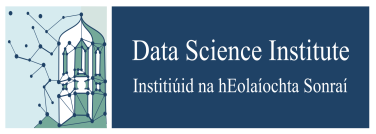
\includegraphics[width=\linewidth]{LT-EDI-2025/sponsor_logos/DSI_logo.png}
      \end{minipage}\hspace{0.05\linewidth}
          \begin{minipage}[c][0.21\linewidth][c]{0.21\linewidth}
        
\includegraphics[width=\linewidth]{LT-EDI-2025/sponsor_logos/uja.png}
      \end{minipage}\hspace{0.05\linewidth}
    
    \end{samepage}

  \bigskip
  \bigskip
\newpage


%%%%%%%%%%%%%
% Copyright %
%%%%%%%%%%%%%
\phantomsection
\addcontentsline{toc}{section}{Copyright}
\vspace*{11cm}
{\large

\noindent
\textcopyright 2025 Association for Computational Linguistics\\

\vspace*{2cm}
\noindent
Order copies of this and other ACL proceedings from:

\vspace*{1cm}
\begin{tabular}{p{1.5cm}l}
& Association for Computational Linguistics (ACL)\\
& 317 Sidney Baker St. S \\
& Suite 400 - 134\\
& Kerrville, TX 78028\\
& USA\\
& Tel: +1-855-225-1962\\
&{\tt acl@aclweb.org}\\
\end{tabular}

\vspace*{1cm}
ISBN None
}
\newpage


%%%%%%%%%%%%
% Prefaces %
%%%%%%%%%%%%
  \phantomsection
  \addcontentsline{toc}{section}{Introduction}
  \begin{center}
   { \Large \textbf{Introduction}}
  \end{center}
  \vspace*{0.5cm}
  We are excited to welcome you to the Fifth Workshop on Language Technology for Equality, Diversity, Inclusion (LT-EDI-2025), the 5th Conference on Language, Data and Knowledge (LDK). This year, the workshop will be held in a hybrid format (both online and Workshops will take place at Palazzo del Mediterraneo on 9th September 2025, while the main venue for the conference will be Palazzo Corigliano, on 10th - 11th September 2025, located in the Naples, Italy. With the rapid advancement of technology, digital communication has become a central part of daily life. While many globally dominant languages have successfully transitioned into the digital era, numerous regional and low-resource languages continue to face significant technological challenges. Equality, Diversity and Inclusion (EDI) is an important agenda across every field throughout the world. Language as a major part of communication should be inclusive and treat everyone with equality. Today’s large internet community uses language technology (LT) and has a direct impact on people across the globe. EDI is crucial to ensure everyone is valued and included, so it is necessary to build LT that serves this purpose. Recent results have shown that big data and deep learning are entrenching existing biases and that some algorithms are even naturally biased due to problems such as ‘regression to the mode’. Our focus is on creating LT that will be more inclusive of gender, racial, sexual orientation, persons with disability. The workshop will focus on creating speech and language technology to address EDI not only in English, but also in less resourced languages. The workshop received a total of 40 active submissions. Reviewer recruitment was highly effective, with 232 out of 249 invited reviewers accepting the invitation. Of the 270 assigned reviews, 117 were completed, resulting in a review submission rate of 43.33\%. Additionally, 41.67\% of reviewers (100 out of 240) completed all their assigned reviews. A majority of submissions (65\%, or 26 out of 40) received at least three reviews, ensuring a robust evaluation process. Decisions were finalized for all submissions (100\%), leading to an acceptance rate of 95\% (38 papers). This included 6 papers (15\%) accepted for oral presentations and 32 papers (80\%) accepted for poster presentations. Only 2 submissions (5\%) were rejected. There were no withdrawn submissions, and only one paper was desk rejected. These metrics reflect a thorough and inclusive review process, driven by active reviewer participation and a strong commitment to quality.
  \newpage

%%%%%%%%%%%%%%%%%%%%%%%%
% Organizing Committee %
%%%%%%%%%%%%%%%%%%%%%%%%

%%%%%%%%%%%%%%%%%%%%%
% Program Committee %
%%%%%%%%%%%%%%%%%%%%%
\phantomsection
\addcontentsline{toc}{section}{Program Committee}
\begin{center}
\Large \textbf{Program Committee}
\end{center}
\vspace*{1cm}
\begin{description}
  \item{\bf Program Chairs}\vspace{2mm}\\
            Bharathi Raja Chakravarthi, University of Galway, Ireland\\
          Bharathi B, Sri Sivasubramaniya Nadar College of Engineering, India\\
          Paul Buitelaar, University of Galway, Ireland\\
          Thenmozhi Durairaj, Sri Sivasubramaniya Nadar College of Engineering, India\\
          Miguel Ángel García Cumbreras, University of Jaén, Spain\\
          Salud María Jiménez-Zafra, Universidad de Jaén, Spain\\
      
  \item{\bf Publication Chairs}\vspace{2mm}\\
            Prasanna Kumar Kumaresan, Data Science Institute, University of Galway, Ireland\\
          Shunmuga Priya Muthusamy Chinnan, Data Science Institute, University of Galway, Ireland\\
      
  \item{\bf Reviewers}\vspace{2mm}\\
                    A. Justin Gopinath, Vellore Institute of Technology, India\\
              Abdullah Al Nahian, Shahjalal University of Science and Technology, Bangladesh\\
              Abdur Rahman, Shahjalal University of Science and Technology, Bangladesh\\
              Abirami Jayaraman, Sri Sivasubramaniya Nadar College of Engineering, India\\
              Adeep Hande, Comcast Applied AI, USA\\
              Aishwarya Selvamurugan, Sri Eshwar College of Engineering, India\\
              Amit Jaspal, Facebook, Inc.\\
              Angel Deborah S, Sri Sivasubramaniya Nadar College of Engineering, India\\
              Anusha M D Gowda, University of Mysore, India\\
              Ariful Islam, Chittagong University of Engineering and Technology, Bangladesh\\
              Aruna Devi Shanmugam, Sri Sivasubramaniya Nadar College of Engineering, India\\
              Arunaggiri Pandian Karunanidhi, Micron Technology, Inc.\\
              Asha Hegde, Mangalore University, India\\
              Ashim Dey, Chittagong University of Engineering and Technology, Bangladesh\\
              Ashok Yadav, Indian Institute of Information Technology, Allahabad, India\\
              Ashraful Islam Paran, Chittagong University of Engineering and Technology, Bangladesh\\
              Avaneesh Koushik, Sri Sivasubramaniya Nadar College of Engineering, India\\
              Bagavathi C, Amrita Vishwa Vidyapeetham, India\\
              Belo Abhigyan, University of Delhi, India\\
              Bhuvaneswari Sivagnanam, Central University of Tamil Nadu, India\\
              Boomika E, RMK Engineering College, India\\
              Burugu Rahul, Amrita Vishwa Vidyapeetham, India\\
              Deeptanshu Jha, IEEE, India\\
              Dipanjan Saha, Jadavpur University, India\\
              Dondluru Keerthana, Amrita Vishwa Vidyapeetham, India\\
              Durga Prasad Manukonda, ASRlytics, USA\\
              Fred Philippy, University of Luxemburg and Zortify S.A., Luxembourg\\
              Ganesh Sundhar S, Amrita Vishwa Vidyapeetham, India\\
              Geetha M P, Vellore Institute of Technology, India\\
              Gersome Shimi, Madras Christian College, India\\
              Girma Yohannis Bade, Addis Ababa University, Ethiopia\\
              Gnanasabesan G, Amrita Vishwa Vidyapeetham, India\\
              Hari Krishnan N, Amrita Vishwa Vidyapeetham, India\\
              Harshita Sharma, Institute of Informatics and Communication, India\\
              Hasan Murad, Chittagong University of Engineering and Technology, Bangladesh\\
              Hosahalli Lakshmaiah Shashirekha, Mangalore University, India\\
              Jayanth Jeyadevaswamy, University of Galway, Ireland\\
              Jobin Jose, Indian Institute of Information Technology, Kottayam, India\\
              Jyothish Lal G, Amrita Vishwa Vidyapeetham, India\\
              Kasu Sai Kartheek Reddy, Indian Institute of Technology Tirupati, India\\
              Keerthana Nnl, Vellore Institute of Technology, India\\
              Lalith Kishore V P, RMK Engineering College, India\\
              Luxshan Thavarasa, University of Moratuwa, Sri Lanka\\
              Md.mahadi Rahman, Chittagong University of Engineering and Technology, Bangladesh\\
              Mahankali Sri Ram Krishna, Amrita Vishwa Vidyapeetham, India\\
              Mahfuz Ahmed Anik, Shahjalal University of Science and Technology, Bangladesh\\
              Mahir Absar Khan, Shahjalal University of Science and Technology, Bangladesh\\
              Manan Buddhadev, Rochester Institute of Technology, USA\\
              Md Minhazul Kabir, Chittagong University of Engineering and Technology, Bangladesh\\
              Md Mizanur Rahman, Chittagong University of Engineering and Technology, Bangladesh\\
              Md Ayon Mia, Dhaka International University, Bangladesh\\
              Md. Refaj Hossan, Chittagong University of Engineering and Technology, Bangladesh\\
              Md. Mubasshir Naib, Chittagong University of Engineering and Technology, Bangladesh\\
              Mikhail Krasitskii, Instituto Politécnico Nacional, Mexico\\
              Minhaz Chowdhury, Shahjalal University of Science and Technology, Bangladesh\\
              Minoru Sasaki, Ibaraki University, Japan\\
              Miriam Butt, University of Konstanz, Germany\\
              Mithun M, Sri Eshwar College of Engineering, India\\
              Mohan Raj M A, RMK Engineering College, India\\
              Mohan Raj, Monash University, Australia\\
              Monorama Swain, Indian Institute of Information Technology, Kurnool, India\\
              Moogambigai A, Sri Sivasubramaniya Nadar College of Engineering, India\\
              Mostafa Rahgouy, Auburn University, USA\\
              Mugilkrishna D U, Sri Sivasubramaniya Nadar College of Engineering, India\\
              N.nasurudeen Ahamed, United Arab Emirates University, UAE\\
              Nida Hafeez, Instituto Politécnico Nacional, Mexico\\
              Nishanth.s, Amrita Vishwa Vidyapeetham, India\\
              Nitin Nikamanth Appiah Balaji, Hexion Inc.\\
              Pandiarajan D, Sri Sivasubramaniya Nadar College of Engineering, India\\
              Payal Godhani, Oracle, India\\
              Premjith B, Amrita Vishwa Vidyapeetham, India\\
              Priyanka Ashokan, Sree Chitra Thirunal College of Engineering, India\\
              Radhika K T, National Institute of Technology Trichy and Institute of Printing Technology and Government Polytechnic College, India\\
              Rahatun Nesa Priti, Shahjalal University of Science and Technology, Bangladesh\\
              Rajalakshmi Sivanaiah, Sri Sivasubramaniya Nadar College of Engineering, India\\
              Rajeswarirajasekar, Sri Sivasubramaniya Nadar Institutions, India\\
              Raksha Adyanthaya, Yenepoya Institute Of Arts, Science, Commerce and Management, India\\
              Ratnavel Rajalakshmi, Vellore Institute of Technology, India\\
              Ravi Teja Potla, NVIDIA, USA\\
              Sabik Aftahee, Chittagong University of Engineering and Technology, Bangladesh\\
              Sai Koneru, Pennsylvania State University, USA\\
              Sarbajeet Pattanaik, Indian Institute of Information Technology, Allahabad, India\\
              Satya Subrahmanya Gautama Shastry Bulusu Venkata, George Mason University, USA\\
              Saurabh Aggarwal, Autodesk, India\\
              Sayan Das, Jadavpur University, India\\
              Shreyas Karthik, Sri Sivasubramaniya Nadar College of Engineering, India\\
              Shruthi Rengarajan, Amrita Vishwa Vidyapeetham, India\\
              Shruthikaa V, Amrita Vishwa Vidyapeetham, India\\
              Sidney Wong, University of Canterbury, New Zealand\\
              Simran, Institute of Informatics and Communication, India\\
              Sitara K, National Institute of Technology Tiruchirappalli, India\\
              Soham Chaudhuri, Jadavpur University, India\\
              Somsubhra De, Indian Institute of Technology, Roorkee\\
              Sreeja K, Sri Sivasubramaniya Nadar College of Engineering, India\\
              Sripriya N, Sri Sivasubramaniya Nadar College of Engineering, India\\
              Tanisha Sriram, Sri Sivasubramaniya Nadar College of Engineering, India\\
              Tareque Md Hanif, Shahjalal University of Science and Technology, Bangladesh\\
              Tewodros Achamaleh, University of Gondar, Ethiopia\\
              Tolulope Olalekan Abiola, Instituto Politécnico Nacional, Mexico\\
              Trina Chakraborty, Shahjalal University of Science and Technology, Bangladesh\\
              Udoy Das, Chittagong University of Engineering and Technology, Bangladesh\\
              Uma Jothi, Amrita Vishwa Vidyapeetham, India\\
              Vajratiya Vajrobol, Vellore Institute of Technology, India\\
            % 
\end{description}
\newpage

%%%%%%%%%%%%%%%%%
% Invited Talks %
%%%%%%%%%%%%%%%%%
  \phantomsection
  \addcontentsline{toc}{section}{Keynote Talk: To be Done}
  \begin{center}
          {\Large \textbf{Keynote Talk}\\}
      {\LARGE \textbf{To be Done}\\}
        \vspace*{0.5cm}
    %\begin{minipage}[c][0.35\linewidth][c]{0.35\linewidth}
     % \end{minipage}\\
    \textbf{Remi Denton}\\
        Google, AI, Society, and Culture (TASC)\\
        
        
        \textbf{2025-09-09 09:15} -- 
                Room: \textbf{Palazzo del Mediterraneo, Naples, Italy}\\
        
  \end{center}

  \vspace*{0.2cm}
    \textbf{Abstract:} To be Done\\
  \newline
  
    \textbf{Bio:} Remi Denton, Staff Research Scientist, Google, AI, Society, and Culture (TASC). 
  \newpage
    \phantomsection
  \addcontentsline{toc}{section}{Keynote Talk: To be Done}
  \begin{center}
          {\Large \textbf{Keynote Talk}\\}
      {\LARGE \textbf{To be Done}\\}
        \vspace*{0.5cm}
    %\begin{minipage}[c][0.35\linewidth][c]{0.35\linewidth}
     % \end{minipage}\\
    \textbf{Momchil Hardalov}\\
        Amazon AWS AI Labs\\
        
        
        \textbf{2025-09-09 09:15} -- 
                Room: \textbf{Palazzo del Mediterraneo, Naples, Italy}\\
        
  \end{center}

  \vspace*{0.2cm}
    \textbf{Abstract:} \\
  \newline
  
    \textbf{Bio:} Momchil Hardalov, Applied Scientist in Natural Language Processing (NLP), Amazon AWS AI Labs
  \newpage
  

%%%%%%%%%%%%%%%%%
% Panels %
%%%%%%%%%%%%%%%%%

%%%%%%%%%%%%%%%
% Special Additional Pages %
%%%%%%%%%%%%%%%

%%%%%%%%%%%%%%%%%%%%%
% Table of Contents %
%%%%%%%%%%%%%%%%%%%%%
\phantomsection
\addcontentsline{toc}{section}{Table of Contents}
\newpage  % Empty page before TOC
\pagestyle{plain}
\begin{center}
{\Large \textbf{Table of Contents}}
\end{center}
\vspace*{1em}
\newcommand\page[1]{\rightskip=25pt \dotfill\rlap{\hbox to 25pt{\hfill#1}}\par}
\begin{itemize}[leftmargin=*,label={}]
       \item \hyperlink{page.1}{\emph{SSNCSE@LT-EDI-2025:Detecting Misogyny Memes using Pretrained Deep Learning models}}\\ \hspace*{2em} Sreeja K\index{K} and Bharathi B\index{B}\dotfill \hyperlink{page.1}{1}
       \item \hyperlink{page.6}{\emph{SSNCSE@LT-EDI-2025:Speech Recognition for Vulnerable Individuals in Tamil}}\\ \hspace*{2em} Sreeja K\index{K} and Bharathi B\index{B}\dotfill \hyperlink{page.6}{6}
       \item \hyperlink{page.11}{\emph{CrewX@LT-EDI-2025: Transformer-Based Tamil ASR Fine-Tuning with AVMD Denoising and GRU-VAD for Enhanced Transcription Accuracy}}\\ \hspace*{2em} Ganesh Sundhar S\index{S}, Hari Krishnan N\index{N}, Arun Prasad T D\index{D}, Shruthikaa V\index{V} and Jyothish Lal G\index{G}\dotfill \hyperlink{page.11}{11}
       \item \hyperlink{page.17}{\emph{JUNLP@LT-EDI-2025: Efficient Low-Rank Adaptation of Whisper for Inclusive Tamil Speech Recognition Targeting Vulnerable Populations}}\\ \hspace*{2em} Priyobroto Acharya\index{Acharya}, Soham Chaudhuri\index{Chaudhuri}, Sayan Das\index{Das}, Dipanjan Saha\index{Saha} and Dipankar Das\index{Das}\dotfill \hyperlink{page.17}{17}
       \item \hyperlink{page.26}{\emph{SKVtrio@LT-EDI-2025: Hybrid TF-IDF and BERT Embeddings for  Multilingual Homophobia and Transphobia Detection in Social Media  Comments}}\\ \hspace*{2em} Konkimalla Laxmi Vignesh\index{Vignesh}, Mahankali Sri Ram Krishna\index{Krishna}, Dondluru Keerthana\index{Keerthana} and Premjith B\index{B}\dotfill \hyperlink{page.26}{26}
       \item \hyperlink{page.31}{\emph{Dll5143A@LT-EDI 2025: Bias-Aware Detection of Racial Hoaxes in Code-Mixed Social Media Data (BaCoHoax)}}\\ \hspace*{2em} Ashok Yadav\index{Yadav} and Vrijendra Singh\index{Singh}\dotfill \hyperlink{page.31}{31}
       \item \hyperlink{page.39}{\emph{Hope\_for\_best@LT-EDI 2025: Detecting Racial Hoaxes in Code-Mixed Hindi-English Social Media Data using a multi-phase fine-tuning strategy}}\\ \hspace*{2em} Abhishek Singh Yadav\index{Yadav}, Deepawali Sharma\index{Sharma}, Aakash Singh\index{Singh} and Vivek Kumar Singh\index{Singh}\dotfill \hyperlink{page.39}{39}
       \item \hyperlink{page.47}{\emph{CVF-NITT@LT-EDI-2025:MisogynyDetection}}\\ \hspace*{2em} Radhika K T\index{T} and Sitara K\index{K}\dotfill \hyperlink{page.47}{47}
       \item \hyperlink{page.54}{\emph{Wise@LT-EDI-2025: Combining Classical and Neural Representations with Multi-scale Ensemble Learning for Code-mixed Hate Speech Detection}}\\ \hspace*{2em} Ganesh Sundhar S\index{S}, Durai Singh K\index{K}, Gnanasabesan G\index{G}, Hari Krishnan N\index{N} and MC Dhanush\index{Dhanush}\dotfill \hyperlink{page.54}{54}
       \item \hyperlink{page.63}{\emph{CUET's\_White\_Walkers@LT-EDI 2025: Racial Hoax Detection in Code-Mixed on Social Media Data}}\\ \hspace*{2em} Md Mizanur Rahman\index{Rahman}, Jidan Al Abrar\index{Abrar}, Md Siddikul Imam Kawser\index{Kawser}, Ariful Islam\index{Islam}, Md. Mubasshir Naib\index{Naib} and Hasan Murad\index{Murad}\dotfill \hyperlink{page.63}{63}
       \item \hyperlink{page.68}{\emph{CUET's\_White\_Walkers@LT-EDI-2025: A Multimodal Framework for the Detection of Misogynistic Memes in Chinese Online Content}}\\ \hspace*{2em} Md. Mubasshir Naib\index{Naib}, Md Mizanur Rahman\index{Rahman}, Jidan Al Abrar\index{Abrar}, Md Mehedi Hasan\index{Hasan}, Md Siddikul Imam Kawser\index{Kawser} and Mohammad Shamsul Arefin\index{Arefin}\dotfill \hyperlink{page.68}{68}
       \item \hyperlink{page.75}{\emph{CUET's\_White\_Walkers@LT-EDI 2025: Transformer-Based Model for the Detection of Caste and Migration Hate Speech}}\\ \hspace*{2em} Jidan Al Abrar\index{Abrar}, Md Mizanur Rahman\index{Rahman}, Ariful Islam\index{Islam}, Md Mehedi Hasan\index{Hasan}, Md. Mubasshir Naib\index{Naib} and Mohammad Shamsul Arefin\index{Arefin}\dotfill \hyperlink{page.75}{75}
       \item \hyperlink{page.80}{\emph{NS@LT-EDI-2025 CasteMigration based hate speech Detection}}\\ \hspace*{2em} Nishanth.S Nishanth.S\index{Nishanth.S}, Shruthi Rengarajan\index{Rengarajan} and Sachin Kumar S\index{S}\dotfill \hyperlink{page.80}{80}
       \item \hyperlink{page.84}{\emph{SSN\_IT\_HATE@LT-EDI-2025: Caste and Migration Hate Speech Detection}}\\ \hspace*{2em} Maria Nancy C\index{C}, Radha N\index{N} and Swathika R\index{R}\dotfill \hyperlink{page.84}{84}
       \item \hyperlink{page.90}{\emph{ItsAllGoodMan@LT-EDI-2025: Fusing TF-IDF and MuRIL Embeddings for Detecting Caste and Migration Hate Speech}}\\ \hspace*{2em} Amritha Nandini K L\index{L}, Vishal S\index{S}, Giri Prasath R\index{R}, Anerud Thiyagarajan\index{Thiyagarajan} and Sachin Kumar S\index{S}\dotfill \hyperlink{page.90}{90}
       \item \hyperlink{page.95}{\emph{NSR\_LT-EDI-2025 Automatic speech recognition in Tamil}}\\ \hspace*{2em} Nishanth.S Nishanth.S\index{Nishanth.S}, Shruthi Rengarajan\index{Rengarajan}, Burugu Rahul\index{Rahul} and Jyothish Lal G\index{G}\dotfill \hyperlink{page.95}{95}
       \item \hyperlink{page.100}{\emph{Solvers@LT-EDI-2025: Caste and Migration Hate Speech Detection in Tamil-English Code-Mixed Text}}\\ \hspace*{2em} Ananthakumar S\index{S}, Bharath P\index{P}, Devasri A\index{A}, Anirudh Sriram K S\index{S} and Mohanapriya K T\index{T}\dotfill \hyperlink{page.100}{100}
       \item \hyperlink{page.105}{\emph{CUET\_N317@LT-EDI2025: Detecting Hate Speech Related to Caste and Migration with Transformer Models}}\\ \hspace*{2em} Md. Nur Siddik Ruman\index{Ruman}, Md. Tahfim Juwel Chowdhury\index{Chowdhury} and Hasan Murad\index{Murad}\dotfill \hyperlink{page.105}{105}
       \item \hyperlink{page.111}{\emph{KEC-Elite-Analysts@LT-EDI 2025: Leveraging Deep Learning for Racial Hoax Detection in Code-Mixed Hindi-English Tweets}}\\ \hspace*{2em} Malliga Subramanian\index{Subramanian}, Aruna A\index{A}, Amudhavan M\index{M}, Jahaganapathi S\index{S} and Kogilavani Shanmugavadivel\index{Shanmugavadivel}\dotfill \hyperlink{page.111}{111}
       \item \hyperlink{page.116}{\emph{Team\_Luminaries\_0227@LT-EDI-2025: A Transformer-Based Fusion Approach to Misogyny Detection in Chinese Memes}}\\ \hspace*{2em} Adnan Faisal\index{Faisal}, Shiti Chowdhury\index{Chowdhury}, Momtazul Arefin Labib\index{Labib} and Hasan Murad\index{Murad}\dotfill \hyperlink{page.116}{116}
       \item \hyperlink{page.121}{\emph{Hinterwelt@LT-EDI 2025: A Transformer-Based Approach for Identifying Racial Hoaxes in Code-Mixed Hindi-English Social Media Narratives}}\\ \hspace*{2em} Md. Abdur Rahman\index{Rahman}, MD AL Amin\index{Amin}, Sabik Aftahee\index{Aftahee} and Md Ashiqur Rahman\index{Rahman}\dotfill \hyperlink{page.121}{121}
       \item \hyperlink{page.127}{\emph{CUET\_12033@LT-EDI-2025: Misogyny Detection}}\\ \hspace*{2em} Mehreen Rahman\index{Rahman}, Faozia Fariha\index{Fariha}, Nabilah Tabassum\index{Tabassum}, Samia Rahman\index{Rahman} and Hasan Murad\index{Murad}\dotfill \hyperlink{page.127}{127}
       \item \hyperlink{page.133}{\emph{CUET\_Blitz\_Aces@LT-EDI-2025: Leveraging Transformer Ensembles and Majority Voting for Hate Speech Detection}}\\ \hspace*{2em} Shahriar Farhan Karim\index{Karim}, Anower Sha Shajalal Kashmary\index{Kashmary} and Hasan Murad\index{Murad}\dotfill \hyperlink{page.133}{133}
       \item \hyperlink{page.140}{\emph{Hinterwelt@LT-EDI 2025: A Transformer-Based Detection of Caste and Migration Hate Speech in Tamil Social Media}}\\ \hspace*{2em} MD AL Amin\index{Amin}, Sabik Aftahee\index{Aftahee}, Md. Abdur Rahman\index{Rahman}, Md Sajid Hossain Khan\index{Khan} and Md Ashiqur Rahman\index{Rahman}\dotfill \hyperlink{page.140}{140}
       \item \hyperlink{page.146}{\emph{EM-26@LT-EDI 2025: Detecting Racial Hoaxes in Code-Mixed Social Media Data}}\\ \hspace*{2em} Tewodros Achamaleh\index{Achamaleh}, Fatima Uroosa\index{Uroosa}, Nida Hafeez\index{Hafeez}, Tolulope Olalekan Abiola\index{Abiola}, Mikiyas Mebraihtu\index{Mebraihtu}, Sara Getachew\index{Getachew}, Grigori Sidorov\index{Sidorov} and Rolando Quintero\index{Quintero}\dotfill \hyperlink{page.146}{146}
       \item \hyperlink{page.152}{\emph{EM-26@LT-EDI 2025: Caste and Migration Hate Speech Detection in Tamil-English Code-Mixed Social Media Texts}}\\ \hspace*{2em} Tewodros Achamaleh\index{Achamaleh}, Tolulope Olalekan Abiola\index{Abiola}, Mikiyas Mebraihtu\index{Mebraihtu}, Sara Getachew\index{Getachew} and Grigori Sidorov\index{Sidorov}\dotfill \hyperlink{page.152}{152}
       \item \hyperlink{page.159}{\emph{Hoax Terminators@LT-EDI 2025: CharBERT's dominance over LLM Models in the Detection of Racial Hoaxes in Code-Mixed Hindi-English Social Media Data}}\\ \hspace*{2em} Abrar Hafiz Rabbani\index{Rabbani}, Diganta Das Droba\index{Droba}, Momtazul Arefin Labib\index{Labib}, Samia Rahman\index{Rahman} and Hasan Murad\index{Murad}\dotfill \hyperlink{page.159}{159}
       \item \hyperlink{page.171}{\emph{CUET\_Ignite@LT-EDI-2025: A Multimodal Transformer-Based Approach for Detecting Misogynistic Memes in Chinese Social Media}}\\ \hspace*{2em} MD.Mahadi Rahman\index{Rahman}, Mohammad Minhaj Uddin\index{Uddin}, Mohammad Oman\index{Oman} and Mohammad Shamsul Arefin\index{Arefin}\dotfill \hyperlink{page.171}{171}
       \item \hyperlink{page.177}{\emph{girlsteam@LT-EDI-2025: Caste/Migration based hate speech Detection}}\\ \hspace*{2em} Towshin HOssain Tushi\index{Tushi}, Walisa Alam\index{Alam}, Rehenuma Ilman\index{Ilman} and Samia Rahman\index{Rahman}\dotfill \hyperlink{page.177}{177}
       \item \hyperlink{page.183}{\emph{CUET\_320@LT-EDI-2025: A Multimodal Approach for Misogyny Meme Detection in Chinese Social Media}}\\ \hspace*{2em} Madiha Ahmed Chowdhury\index{Chowdhury}, Lamia Tasnim Khan\index{Khan}, Md.shafiqul Hasan\index{Hasan} and Ashim Dey\index{Dey}\dotfill \hyperlink{page.183}{183}
       \item \hyperlink{page.189}{\emph{Speech Personalization using Parameter Efficient Fine-Tuning for Nepali Speakers}}\\ \hspace*{2em} Kiran Pantha\index{Pantha}, Rupak Raj Ghimire\index{Ghimire} and Bal Krishna Bal\index{Bal}\dotfill \hyperlink{page.189}{189}
       \item \hyperlink{page.199}{\emph{An Overview of the Misogyny Meme Detection Shared Task for Chinese Social Media}}\\ \hspace*{2em} Bharathi Raja Chakravarthi\index{Chakravarthi}, Rahul Ponnusamy\index{Ponnusamy}, Ping Du\index{Du}, Xiaojian Zhuang\index{Zhuang}, Saranya Rajiakodi\index{Rajiakodi}, Paul Buitelaar\index{Buitelaar}, Premjith B\index{B}, Bhuvaneswari Sivagnanam\index{Sivagnanam}, Anshid K A\index{A} and SK Lavanya\index{Lavanya}\dotfill \hyperlink{page.199}{199}
       \item \hyperlink{page.208}{\emph{Findings of the Shared Task Multilingual Bias and Propaganda Annotation in Political Discourse}}\\ \hspace*{2em} Shunmuga Priya Muthusamy Chinnan\index{Chinnan}, Bharathi Raja Chakravarthi\index{Chakravarthi}, Meghann Drury-Grogan\index{Drury-Grogan}, Senthil Kumar B\index{B}, Saranya Rajiakodi\index{Rajiakodi} and Angel Deborah S\index{S}\dotfill \hyperlink{page.208}{208}
       \item \hyperlink{page.214}{\emph{Findings of the Shared Task Caste and Migration Hate Speech Detection}}\\ \hspace*{2em} Saranya Rajiakodi\index{Rajiakodi}, Bharathi Raja Chakravarthi\index{Chakravarthi}, Rahul Ponnusamy\index{Ponnusamy}, Shunmuga Priya Muthusamy Chinnan\index{Chinnan}, Prasanna Kumar Kumaresan\index{Kumaresan}, Sathiyaraj Thangasamy\index{Thangasamy}, Bhuvaneswari Sivagnanam\index{Sivagnanam}, Balasubramanian Palani\index{Palani}, Kogilavani Shanmugavadivel\index{Shanmugavadivel}, Abirami Murugappan\index{Murugappan} and Charmathi Rajkumar\index{Rajkumar}\dotfill \hyperlink{page.214}{214}
       \item \hyperlink{page.221}{\emph{Overview of the Shared Task on Detecting Racial Hoaxes in Code-Mixed Hindi-English Social Media Data}}\\ \hspace*{2em} Bharathi Raja Chakravarthi\index{Chakravarthi}, Prasanna Kumar Kumaresan\index{Kumaresan}, Shanu Dhawale\index{Dhawale}, Saranya Rajiakodi\index{Rajiakodi}, Sajeetha Thavareesan\index{Thavareesan}, Subalalitha Chinnaudayar Navaneethakrishnan\index{Navaneethakrishnan} and Thenmozhi Durairaj\index{Durairaj}\dotfill \hyperlink{page.221}{221}
       \item \hyperlink{page.228}{\emph{Overview of Homophobia and Transphobia Span Detection in Social Media Comments}}\\ \hspace*{2em} Prasanna Kumar Kumaresan\index{Kumaresan}, Bharathi Raja Chakravarthi\index{Chakravarthi}, Ruba Priyadharshini\index{Priyadharshini}, Paul Buitelaar\index{Buitelaar}, Malliga Subramanian\index{Subramanian} and Kishore Kumar Ponnusamy\index{Ponnusamy}\dotfill \hyperlink{page.228}{228}
       \item \hyperlink{page.234}{\emph{Overview of the Fifth Shared Task on Speech Recognition for Vulnerable Individuals in Tamil}}\\ \hspace*{2em} Bharathi B\index{B}, Bharathi Raja Chakravarthi\index{Chakravarthi}, Sripriya N\index{N}, Rajeswari Natarajan\index{Natarajan}, Ratnavel Rajalakshmi\index{Rajalakshmi} and Suhasini S\index{S}\dotfill \hyperlink{page.234}{234}
  \end{itemize}
\newpage

%%%%%%%%%%%
% Program %
%%%%%%%%%%%
\renewcommand{\baselinestretch}{0.87}
\setlength{\parindent}{0in}
\setlength{\parskip}{2ex}

      
          \phantomsection
      \addcontentsline{toc}{section}{Program}
      \begin{center}
      {\Large \textbf{Program}}
      \end{center}
      \vspace*{0.5em}
    
    \begin{tabular}{p{24mm}p{124mm}}
    \multicolumn{2}{l}{\bf Tuesday, September 9, 2025 } \\\\
                  09:00 - 09:15 & \emph{Opening Remarks}\\\\
      
                        09:15 - 09:45 & \emph{To be done}\\\\
      
                        09:45 - 10:30 & \emph{Oral Session 1}\\\\
      
                
                      & \hyperlink{page.189}{\emph{Speech Personalization using Parameter Efficient Fine-Tuning for Nepali Speakers}}\\
        & Kiran Pantha\index{Pantha}, Rupak Raj Ghimire\index{Ghimire} and Bal Krishna Bal\index{Bal}\\\\
                
                      & \hyperlink{page.199}{\emph{An Overview of the Misogyny Meme Detection Shared Task for Chinese Social Media}}\\
        & Bharathi Raja Chakravarthi\index{Chakravarthi}, Rahul Ponnusamy\index{Ponnusamy}, Ping Du\index{Du}, Xiaojian Zhuang\index{Zhuang}, Saranya Rajiakodi\index{Rajiakodi}, Paul Buitelaar\index{Buitelaar}, Premjith B\index{B}, Bhuvaneswari Sivagnanam\index{Sivagnanam}, Anshid K A\index{A} and SK Lavanya\index{Lavanya}\\\\
                
                      & \hyperlink{page.208}{\emph{Findings of the Shared Task Multilingual Bias and Propaganda Annotation in Political Discourse}}\\
        & Shunmuga Priya Muthusamy Chinnan\index{Chinnan}, Bharathi Raja Chakravarthi\index{Chakravarthi}, Meghann Drury-Grogan\index{Drury-Grogan}, Senthil Kumar B\index{B}, Saranya Rajiakodi\index{Rajiakodi} and Angel Deborah S\index{S}\\\\
                        10:30 - 11:00 & \emph{Tea Break}\\\\
      
                        11:00 - 12:00 & \emph{Oral Session 2}\\\\
      
                
                      & \hyperlink{page.214}{\emph{Findings of the Shared Task Caste and Migration Hate Speech Detection}}\\
        & Saranya Rajiakodi\index{Rajiakodi}, Bharathi Raja Chakravarthi\index{Chakravarthi}, Rahul Ponnusamy\index{Ponnusamy}, Shunmuga Priya Muthusamy Chinnan\index{Chinnan}, Prasanna Kumar Kumaresan\index{Kumaresan}, Sathiyaraj Thangasamy\index{Thangasamy}, Bhuvaneswari Sivagnanam\index{Sivagnanam}, Balasubramanian Palani\index{Palani}, Kogilavani Shanmugavadivel\index{Shanmugavadivel}, Abirami Murugappan\index{Murugappan} and Charmathi Rajkumar\index{Rajkumar}\\\\
                
                      & \hyperlink{page.221}{\emph{Overview of the Shared Task on Detecting Racial Hoaxes in Code-Mixed Hindi-English Social Media Data}}\\
        & Bharathi Raja Chakravarthi\index{Chakravarthi}, Prasanna Kumar Kumaresan\index{Kumaresan}, Shanu Dhawale\index{Dhawale}, Saranya Rajiakodi\index{Rajiakodi}, Sajeetha Thavareesan\index{Thavareesan}, Subalalitha Chinnaudayar Navaneethakrishnan\index{Navaneethakrishnan} and Thenmozhi Durairaj\index{Durairaj}\\\\
                
                      & \hyperlink{page.228}{\emph{Overview of Homophobia and Transphobia Span Detection in Social Media Comments}}\\
        & Prasanna Kumar Kumaresan\index{Kumaresan}, Bharathi Raja Chakravarthi\index{Chakravarthi}, Ruba Priyadharshini\index{Priyadharshini}, Paul Buitelaar\index{Buitelaar}, Malliga Subramanian\index{Subramanian} and Kishore Kumar Ponnusamy\index{Ponnusamy}\\\\
                
                      & \hyperlink{page.234}{\emph{Overview of the Fifth Shared Task on Speech Recognition for Vulnerable Individuals in Tamil}}\\
        & Bharathi B\index{B}, Bharathi Raja Chakravarthi\index{Chakravarthi}, Sripriya N\index{N}, Rajeswari Natarajan\index{Natarajan}, Ratnavel Rajalakshmi\index{Rajalakshmi} and Suhasini S\index{S}\\\\
                        12:00 - 13:30 & \emph{Lunch Break}\\\\
      
              \end{tabular}
    \newpage
      
    
    \begin{tabular}{p{24mm}p{124mm}}
    \multicolumn{2}{l}{\bf Tuesday, September 9, 2025 (continued)} \\\\
                  13:30 - 16:00 & \emph{Poster Session}\\\\
      
                
                      & \hyperlink{page.1}{\emph{SSNCSE@LT-EDI-2025:Detecting Misogyny Memes using Pretrained Deep Learning models}}\\
        & Sreeja K\index{K} and Bharathi B\index{B}\\\\
                
                      & \hyperlink{page.6}{\emph{SSNCSE@LT-EDI-2025:Speech Recognition for Vulnerable Individuals in Tamil}}\\
        & Sreeja K\index{K} and Bharathi B\index{B}\\\\
                
                      & \hyperlink{page.11}{\emph{CrewX@LT-EDI-2025: Transformer-Based Tamil ASR Fine-Tuning with AVMD Denoising and GRU-VAD for Enhanced Transcription Accuracy}}\\
        & Ganesh Sundhar S\index{S}, Hari Krishnan N\index{N}, Arun Prasad T D\index{D}, Shruthikaa V\index{V} and Jyothish Lal G\index{G}\\\\
                
                      & \hyperlink{page.17}{\emph{JUNLP@LT-EDI-2025: Efficient Low-Rank Adaptation of Whisper for Inclusive Tamil Speech Recognition Targeting Vulnerable Populations}}\\
        & Priyobroto Acharya\index{Acharya}, Soham Chaudhuri\index{Chaudhuri}, Sayan Das\index{Das}, Dipanjan Saha\index{Saha} and Dipankar Das\index{Das}\\\\
                
                      & \hyperlink{page.26}{\emph{SKVtrio@LT-EDI-2025: Hybrid TF-IDF and BERT Embeddings for  Multilingual Homophobia and Transphobia Detection in Social Media  Comments}}\\
        & Konkimalla Laxmi Vignesh\index{Vignesh}, Mahankali Sri Ram Krishna\index{Krishna}, Dondluru Keerthana\index{Keerthana} and Premjith B\index{B}\\\\
                
                      & \hyperlink{page.31}{\emph{Dll5143A@LT-EDI 2025: Bias-Aware Detection of Racial Hoaxes in Code-Mixed Social Media Data (BaCoHoax)}}\\
        & Ashok Yadav\index{Yadav} and Vrijendra Singh\index{Singh}\\\\
                
                      & \hyperlink{page.39}{\emph{Hope\_for\_best@LT-EDI 2025: Detecting Racial Hoaxes in Code-Mixed Hindi-English Social Media Data using a multi-phase fine-tuning strategy}}\\
        & Abhishek Singh Yadav\index{Yadav}, Deepawali Sharma\index{Sharma}, Aakash Singh\index{Singh} and Vivek Kumar Singh\index{Singh}\\\\
                
                      & \hyperlink{page.47}{\emph{CVF-NITT@LT-EDI-2025:MisogynyDetection}}\\
        & Radhika K T\index{T} and Sitara K\index{K}\\\\
                
                      & \hyperlink{page.54}{\emph{Wise@LT-EDI-2025: Combining Classical and Neural Representations with Multi-scale Ensemble Learning for Code-mixed Hate Speech Detection}}\\
        & Ganesh Sundhar S\index{S}, Durai Singh K\index{K}, Gnanasabesan G\index{G}, Hari Krishnan N\index{N} and MC Dhanush\index{Dhanush}\\\\
                
                      & \hyperlink{page.63}{\emph{CUET's\_White\_Walkers@LT-EDI 2025: Racial Hoax Detection in Code-Mixed on Social Media Data}}\\
        & Md Mizanur Rahman\index{Rahman}, Jidan Al Abrar\index{Abrar}, Md Siddikul Imam Kawser\index{Kawser}, Ariful Islam\index{Islam}, Md. Mubasshir Naib\index{Naib} and Hasan Murad\index{Murad}\\\\
              \end{tabular}
    \newpage
      
    
    \begin{tabular}{p{24mm}p{124mm}}
    \multicolumn{2}{l}{\bf Tuesday, September 9, 2025 (continued)} \\\\
          
                      & \hyperlink{page.68}{\emph{CUET's\_White\_Walkers@LT-EDI-2025: A Multimodal Framework for the Detection of Misogynistic Memes in Chinese Online Content}}\\
        & Md. Mubasshir Naib\index{Naib}, Md Mizanur Rahman\index{Rahman}, Jidan Al Abrar\index{Abrar}, Md Mehedi Hasan\index{Hasan}, Md Siddikul Imam Kawser\index{Kawser} and Mohammad Shamsul Arefin\index{Arefin}\\\\
                
                      & \hyperlink{page.75}{\emph{CUET's\_White\_Walkers@LT-EDI 2025: Transformer-Based Model for the Detection of Caste and Migration Hate Speech}}\\
        & Jidan Al Abrar\index{Abrar}, Md Mizanur Rahman\index{Rahman}, Ariful Islam\index{Islam}, Md Mehedi Hasan\index{Hasan}, Md. Mubasshir Naib\index{Naib} and Mohammad Shamsul Arefin\index{Arefin}\\\\
                
                      & \hyperlink{page.80}{\emph{NS@LT-EDI-2025 CasteMigration based hate speech Detection}}\\
        & Nishanth.S Nishanth.S\index{Nishanth.S}, Shruthi Rengarajan\index{Rengarajan} and Sachin Kumar S\index{S}\\\\
                
                      & \hyperlink{page.84}{\emph{SSN\_IT\_HATE@LT-EDI-2025: Caste and Migration Hate Speech Detection}}\\
        & Maria Nancy C\index{C}, Radha N\index{N} and Swathika R\index{R}\\\\
                
                      & \hyperlink{page.90}{\emph{ItsAllGoodMan@LT-EDI-2025: Fusing TF-IDF and MuRIL Embeddings for Detecting Caste and Migration Hate Speech}}\\
        & Amritha Nandini K L\index{L}, Vishal S\index{S}, Giri Prasath R\index{R}, Anerud Thiyagarajan\index{Thiyagarajan} and Sachin Kumar S\index{S}\\\\
                
                      & \hyperlink{page.95}{\emph{NSR\_LT-EDI-2025 Automatic speech recognition in Tamil}}\\
        & Nishanth.S Nishanth.S\index{Nishanth.S}, Shruthi Rengarajan\index{Rengarajan}, Burugu Rahul\index{Rahul} and Jyothish Lal G\index{G}\\\\
                
                      & \hyperlink{page.100}{\emph{Solvers@LT-EDI-2025: Caste and Migration Hate Speech Detection in Tamil-English Code-Mixed Text}}\\
        & Ananthakumar S\index{S}, Bharath P\index{P}, Devasri A\index{A}, Anirudh Sriram K S\index{S} and Mohanapriya K T\index{T}\\\\
                
                      & \hyperlink{page.105}{\emph{CUET\_N317@LT-EDI2025: Detecting Hate Speech Related to Caste and Migration with Transformer Models}}\\
        & Md. Nur Siddik Ruman\index{Ruman}, Md. Tahfim Juwel Chowdhury\index{Chowdhury} and Hasan Murad\index{Murad}\\\\
                
                      & \hyperlink{page.111}{\emph{KEC-Elite-Analysts@LT-EDI 2025: Leveraging Deep Learning for Racial Hoax Detection in Code-Mixed Hindi-English Tweets}}\\
        & Malliga Subramanian\index{Subramanian}, Aruna A\index{A}, Amudhavan M\index{M}, Jahaganapathi S\index{S} and Kogilavani Shanmugavadivel\index{Shanmugavadivel}\\\\
                
                      & \hyperlink{page.116}{\emph{Team\_Luminaries\_0227@LT-EDI-2025: A Transformer-Based Fusion Approach to Misogyny Detection in Chinese Memes}}\\
        & Adnan Faisal\index{Faisal}, Shiti Chowdhury\index{Chowdhury}, Momtazul Arefin Labib\index{Labib} and Hasan Murad\index{Murad}\\\\
                
                      & \hyperlink{page.121}{\emph{Hinterwelt@LT-EDI 2025: A Transformer-Based Approach for Identifying Racial Hoaxes in Code-Mixed Hindi-English Social Media Narratives}}\\
        & Md. Abdur Rahman\index{Rahman}, MD AL Amin\index{Amin}, Sabik Aftahee\index{Aftahee} and Md Ashiqur Rahman\index{Rahman}\\\\
              \end{tabular}
    \newpage
      
    
    \begin{tabular}{p{24mm}p{124mm}}
    \multicolumn{2}{l}{\bf Tuesday, September 9, 2025 (continued)} \\\\
          
                      & \hyperlink{page.127}{\emph{CUET\_12033@LT-EDI-2025: Misogyny Detection}}\\
        & Mehreen Rahman\index{Rahman}, Faozia Fariha\index{Fariha}, Nabilah Tabassum\index{Tabassum}, Samia Rahman\index{Rahman} and Hasan Murad\index{Murad}\\\\
                
                      & \hyperlink{page.133}{\emph{CUET\_Blitz\_Aces@LT-EDI-2025: Leveraging Transformer Ensembles and Majority Voting for Hate Speech Detection}}\\
        & Shahriar Farhan Karim\index{Karim}, Anower Sha Shajalal Kashmary\index{Kashmary} and Hasan Murad\index{Murad}\\\\
                
                      & \hyperlink{page.140}{\emph{Hinterwelt@LT-EDI 2025: A Transformer-Based Detection of Caste and Migration Hate Speech in Tamil Social Media}}\\
        & MD AL Amin\index{Amin}, Sabik Aftahee\index{Aftahee}, Md. Abdur Rahman\index{Rahman}, Md Sajid Hossain Khan\index{Khan} and Md Ashiqur Rahman\index{Rahman}\\\\
                
                      & \hyperlink{page.146}{\emph{EM-26@LT-EDI 2025: Detecting Racial Hoaxes in Code-Mixed Social Media Data}}\\
        & Tewodros Achamaleh\index{Achamaleh}, Fatima Uroosa\index{Uroosa}, Nida Hafeez\index{Hafeez}, Tolulope Olalekan Abiola\index{Abiola}, Mikiyas Mebraihtu\index{Mebraihtu}, Sara Getachew\index{Getachew}, Grigori Sidorov\index{Sidorov} and Rolando Quintero\index{Quintero}\\\\
                
                      & \hyperlink{page.152}{\emph{EM-26@LT-EDI 2025: Caste and Migration Hate Speech Detection in Tamil-English Code-Mixed Social Media Texts}}\\
        & Tewodros Achamaleh\index{Achamaleh}, Tolulope Olalekan Abiola\index{Abiola}, Mikiyas Mebraihtu\index{Mebraihtu}, Sara Getachew\index{Getachew} and Grigori Sidorov\index{Sidorov}\\\\
                
                      & \hyperlink{page.159}{\emph{Hoax Terminators@LT-EDI 2025: CharBERT's dominance over LLM Models in the Detection of Racial Hoaxes in Code-Mixed Hindi-English Social Media Data}}\\
        & Abrar Hafiz Rabbani\index{Rabbani}, Diganta Das Droba\index{Droba}, Momtazul Arefin Labib\index{Labib}, Samia Rahman\index{Rahman} and Hasan Murad\index{Murad}\\\\
                
                      & \hyperlink{page.171}{\emph{CUET\_Ignite@LT-EDI-2025: A Multimodal Transformer-Based Approach for Detecting Misogynistic Memes in Chinese Social Media}}\\
        & MD.Mahadi Rahman\index{Rahman}, Mohammad Minhaj Uddin\index{Uddin}, Mohammad Oman\index{Oman} and Mohammad Shamsul Arefin\index{Arefin}\\\\
                
                      & \hyperlink{page.177}{\emph{girlsteam@LT-EDI-2025: Caste/Migration based hate speech Detection}}\\
        & Towshin HOssain Tushi\index{Tushi}, Walisa Alam\index{Alam}, Rehenuma Ilman\index{Ilman} and Samia Rahman\index{Rahman}\\\\
                
                      & \hyperlink{page.183}{\emph{CUET\_320@LT-EDI-2025: A Multimodal Approach for Misogyny Meme Detection in Chinese Social Media}}\\
        & Madiha Ahmed Chowdhury\index{Chowdhury}, Lamia Tasnim Khan\index{Khan}, Md.shafiqul Hasan\index{Hasan} and Ashim Dey\index{Dey}\\\\
                        16:00 - 16:15 & \emph{Closing Remarks}\\\\
      
              \end{tabular}
    \newpage
      

  % Flag to generate only front matter or include papers.
%%%%%%%%%%
% Papers %
%%%%%%%%%%
\pagenumbering{arabic}
\setcounter{page}{1}
\renewcommand{\headrulewidth}{0pt}
  \AddToShipoutPicture*{
    \setlength{\unitlength}{1mm}
    \footnotesize

            
    \put(0,13){\parbox[t]{\paperwidth}{\centering
    							\emph{Proceedings of the Fifth Workshop on Language Technology for Equality, Diversity, Inclusion}, pages 1--5 \\
  	  						September 9, 2025 \textcopyright
  							2025 Association for Computational Linguistics}}
  }
  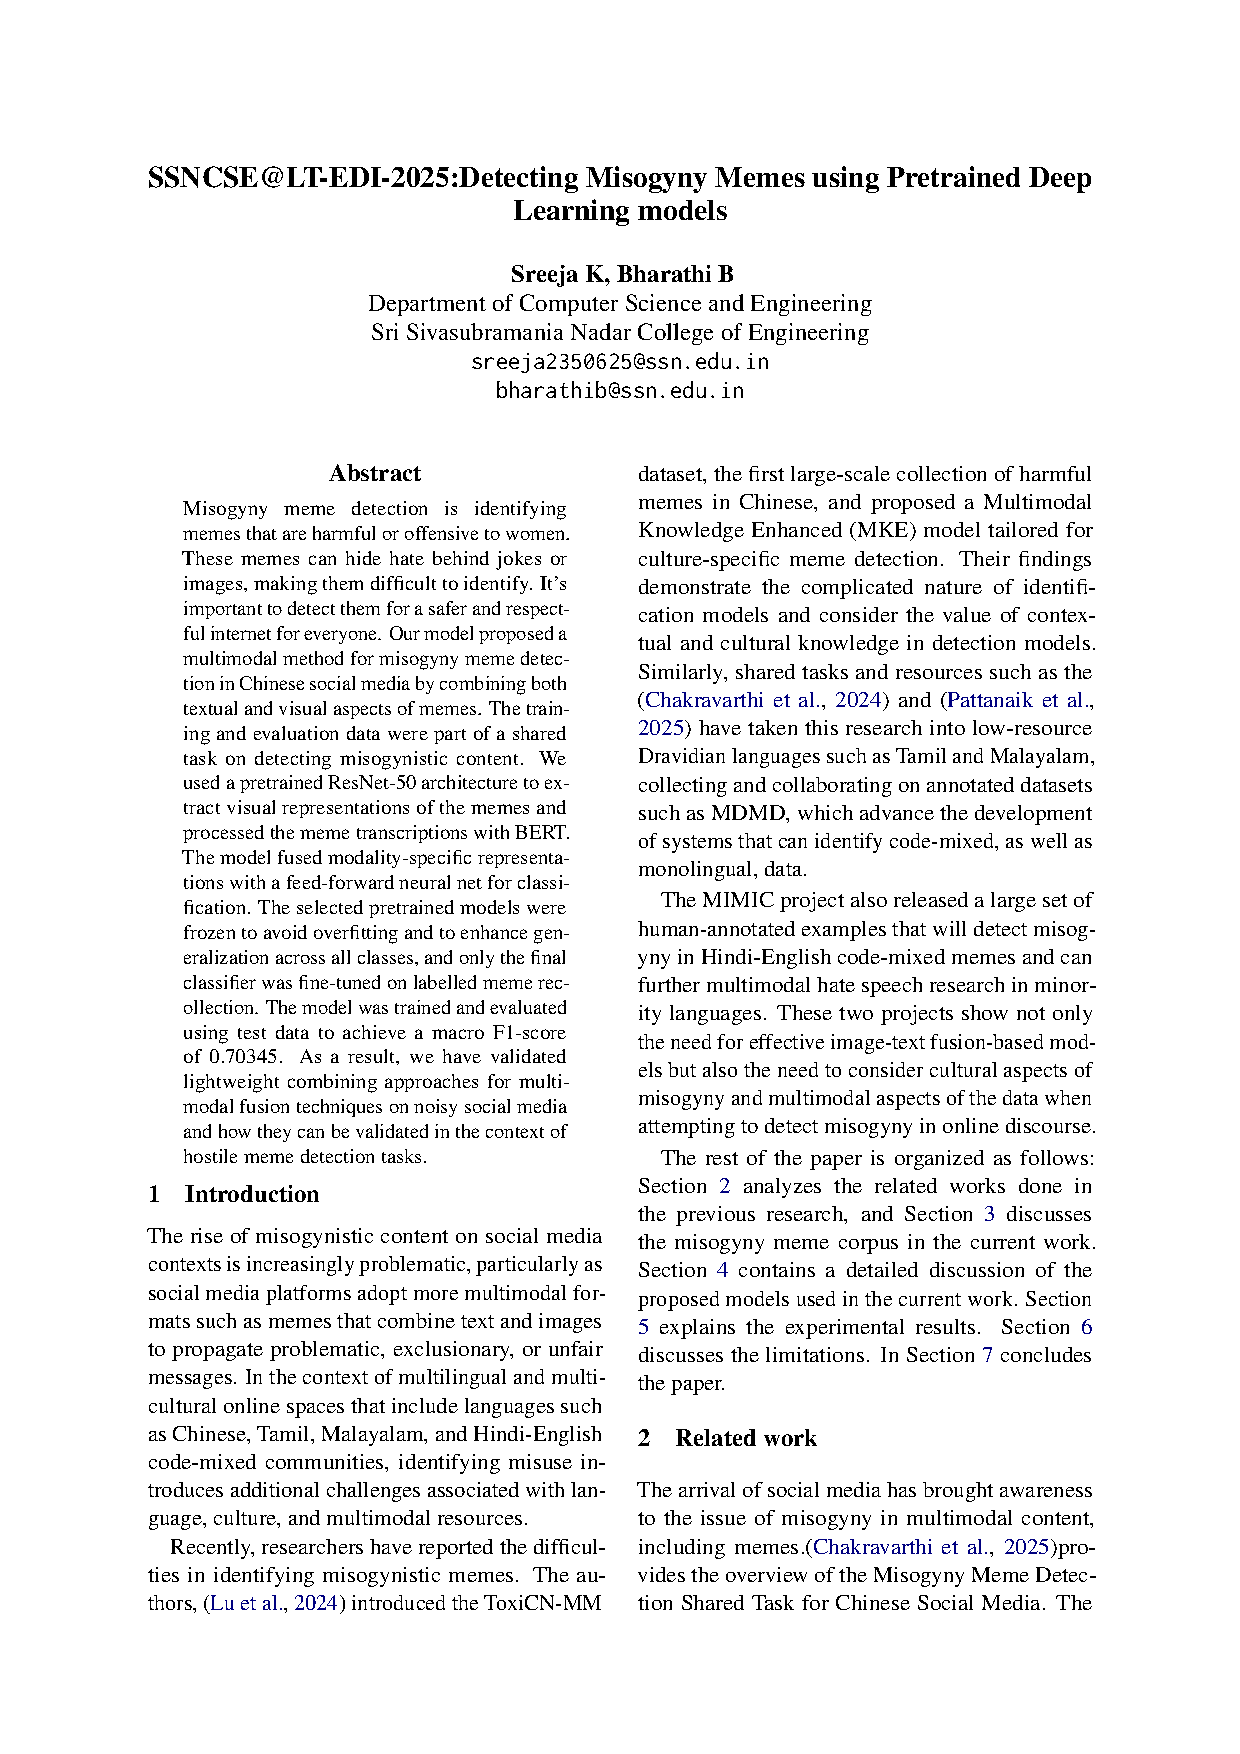
\includepdf[pagecommand={\thispagestyle{plain}},pages=-,addtotoc={1,section,1,{SSNCSE@LT-EDI-2025:Detecting Misogyny Memes using Pretrained Deep Learning models},ref:paper_{1}}]{LT-EDI-2025/papers/1.pdf}
  \AddToShipoutPicture*{
    \setlength{\unitlength}{1mm}
    \footnotesize

            
    \put(0,13){\parbox[t]{\paperwidth}{\centering
    							\emph{Proceedings of the Fifth Workshop on Language Technology for Equality, Diversity, Inclusion}, pages 6--10 \\
  	  						September 9, 2025 \textcopyright
  							2025 Association for Computational Linguistics}}
  }
  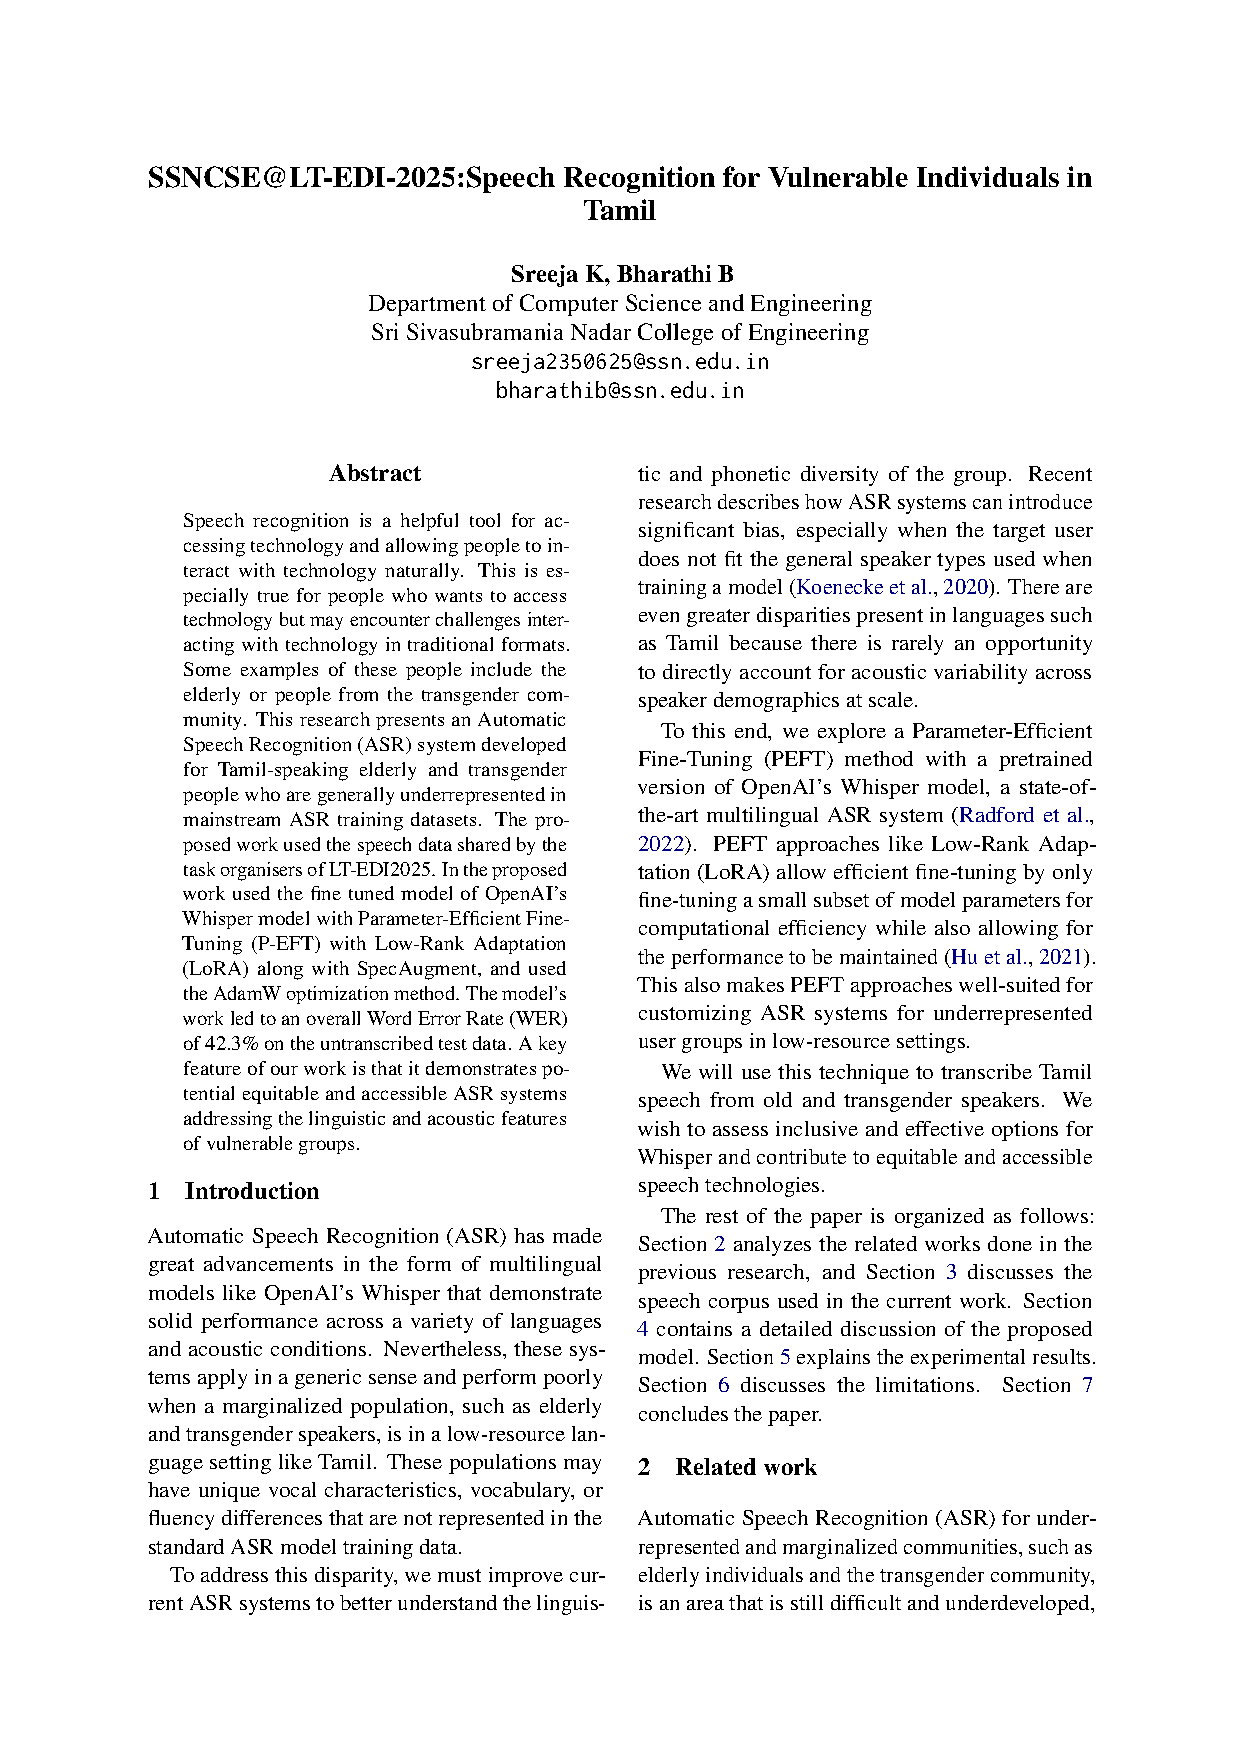
\includepdf[pagecommand={\thispagestyle{plain}},pages=-,addtotoc={1,section,1,{SSNCSE@LT-EDI-2025:Speech Recognition for Vulnerable Individuals in Tamil},ref:paper_{2}}]{LT-EDI-2025/papers/2.pdf}
  \AddToShipoutPicture*{
    \setlength{\unitlength}{1mm}
    \footnotesize

            
    \put(0,13){\parbox[t]{\paperwidth}{\centering
    							\emph{Proceedings of the Fifth Workshop on Language Technology for Equality, Diversity, Inclusion}, pages 11--16 \\
  	  						September 9, 2025 \textcopyright
  							2025 Association for Computational Linguistics}}
  }
  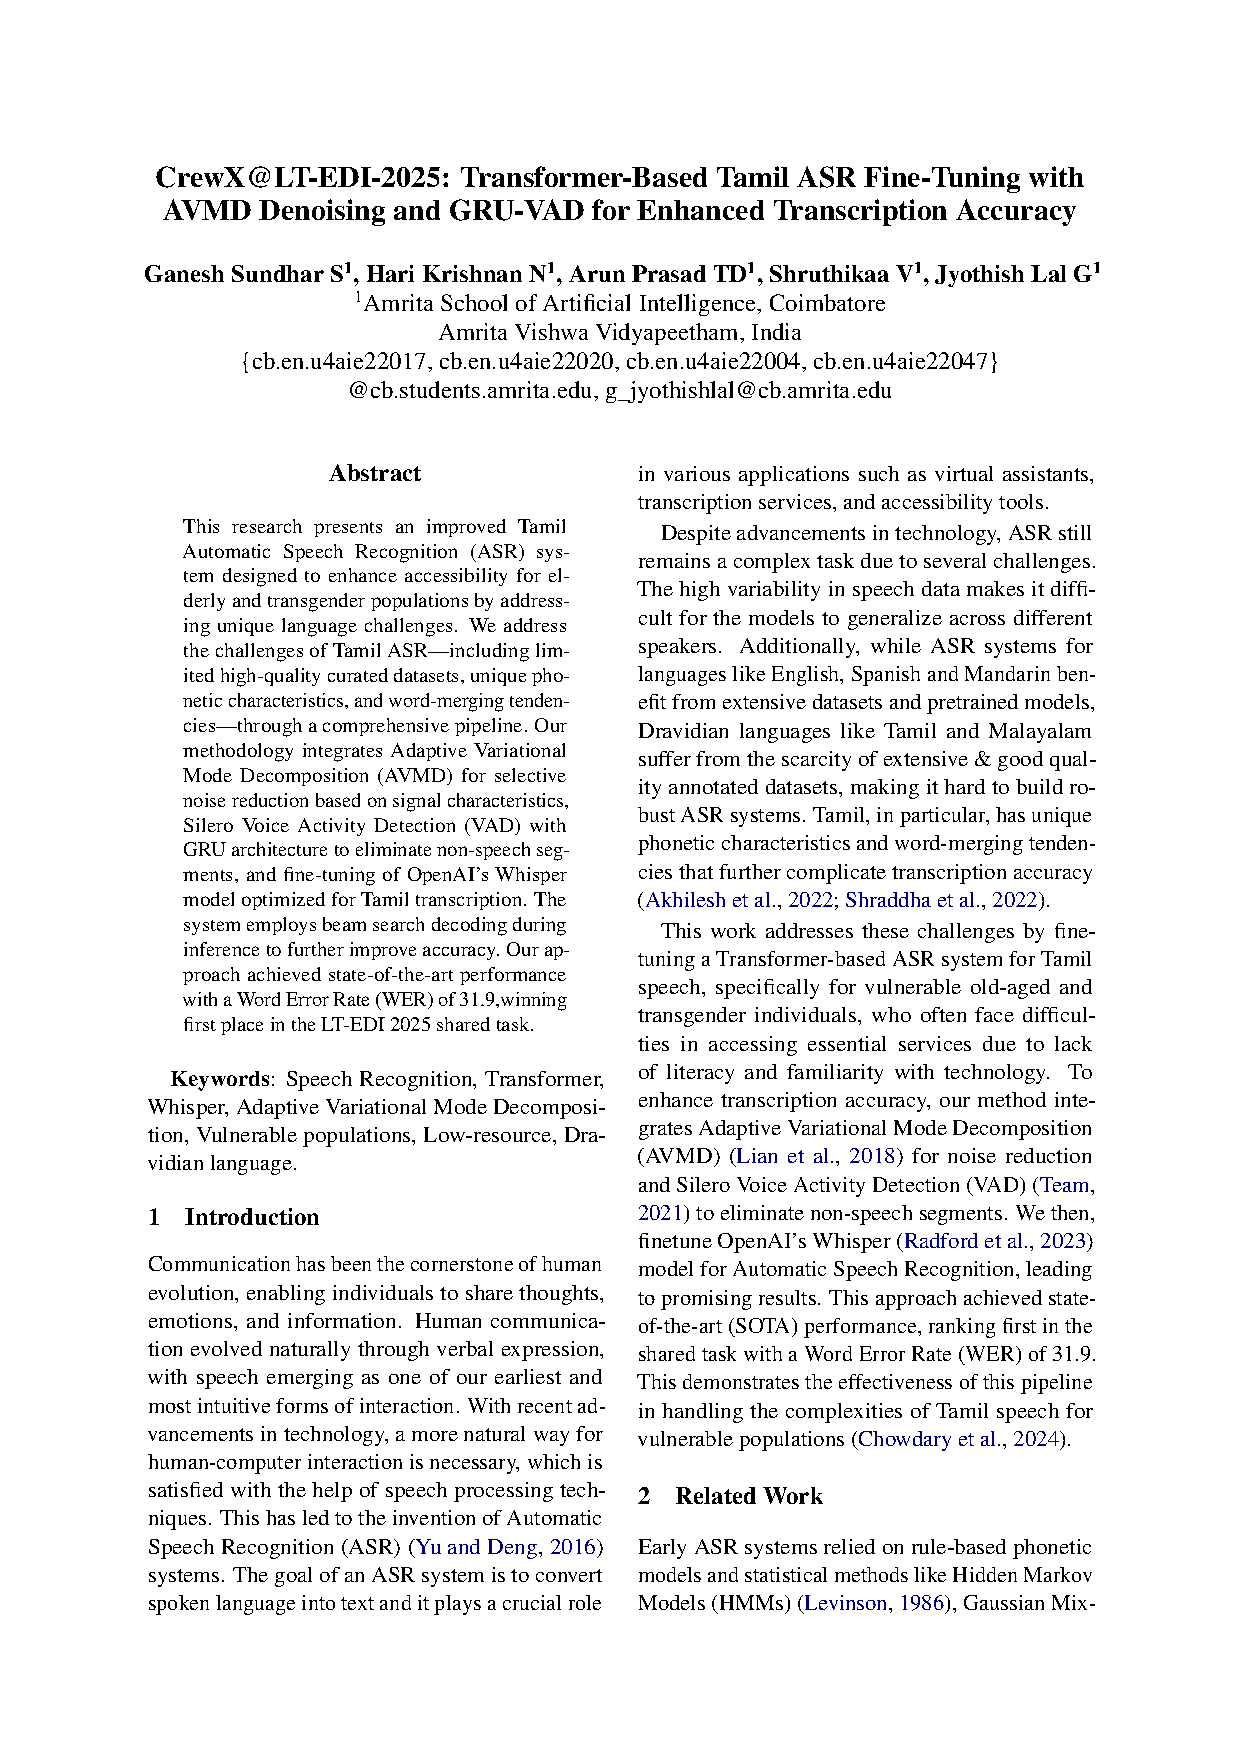
\includepdf[pagecommand={\thispagestyle{plain}},pages=-,addtotoc={1,section,1,{CrewX@LT-EDI-2025: Transformer-Based Tamil ASR Fine-Tuning with AVMD Denoising and GRU-VAD for Enhanced Transcription Accuracy},ref:paper_{4}}]{LT-EDI-2025/papers/4.pdf}
  \AddToShipoutPicture*{
    \setlength{\unitlength}{1mm}
    \footnotesize

            
    \put(0,13){\parbox[t]{\paperwidth}{\centering
    							\emph{Proceedings of the Fifth Workshop on Language Technology for Equality, Diversity, Inclusion}, pages 17--25 \\
  	  						September 9, 2025 \textcopyright
  							2025 Association for Computational Linguistics}}
  }
  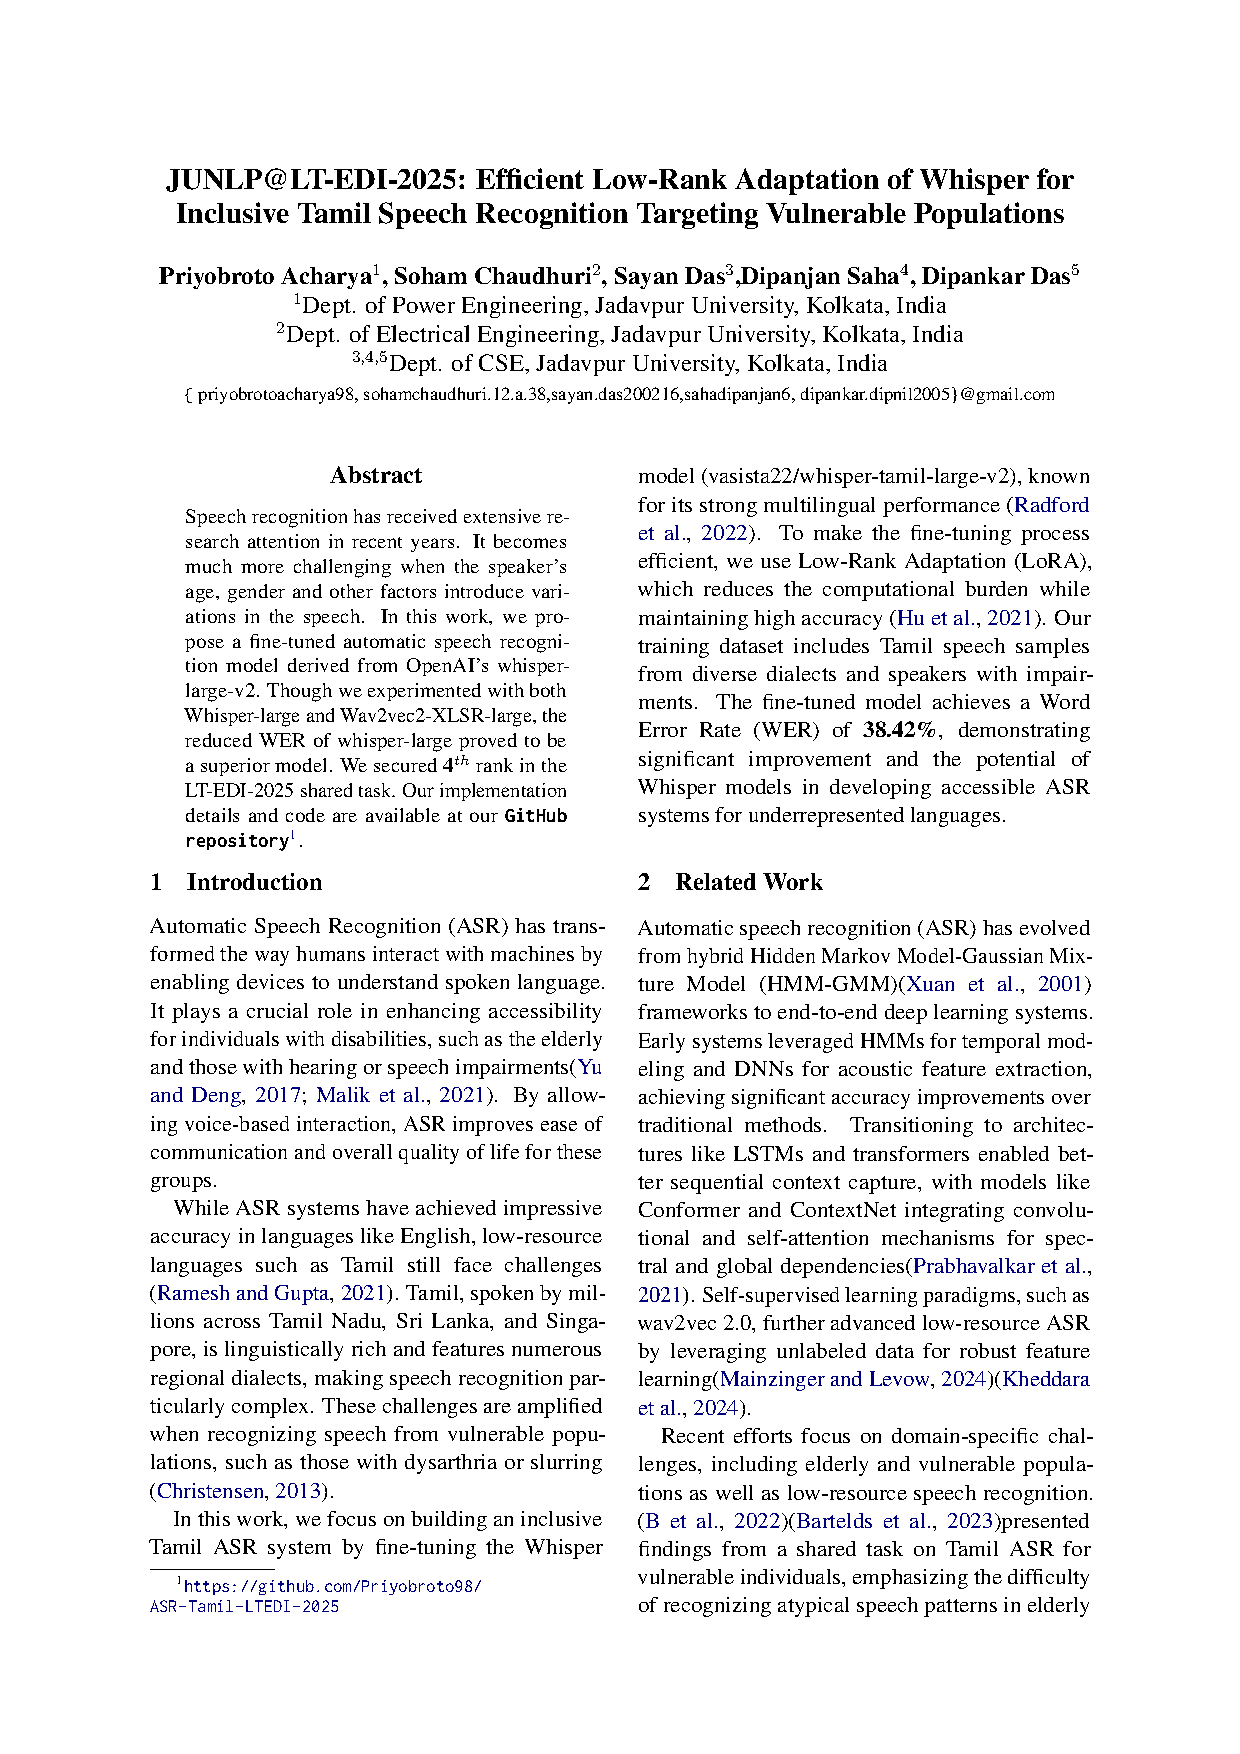
\includepdf[pagecommand={\thispagestyle{plain}},pages=-,addtotoc={1,section,1,{JUNLP@LT-EDI-2025: Efficient Low-Rank Adaptation of Whisper for Inclusive Tamil Speech Recognition Targeting Vulnerable Populations},ref:paper_{5}}]{LT-EDI-2025/papers/5.pdf}
  \AddToShipoutPicture*{
    \setlength{\unitlength}{1mm}
    \footnotesize

            
    \put(0,13){\parbox[t]{\paperwidth}{\centering
    							\emph{Proceedings of the Fifth Workshop on Language Technology for Equality, Diversity, Inclusion}, pages 26--30 \\
  	  						September 9, 2025 \textcopyright
  							2025 Association for Computational Linguistics}}
  }
  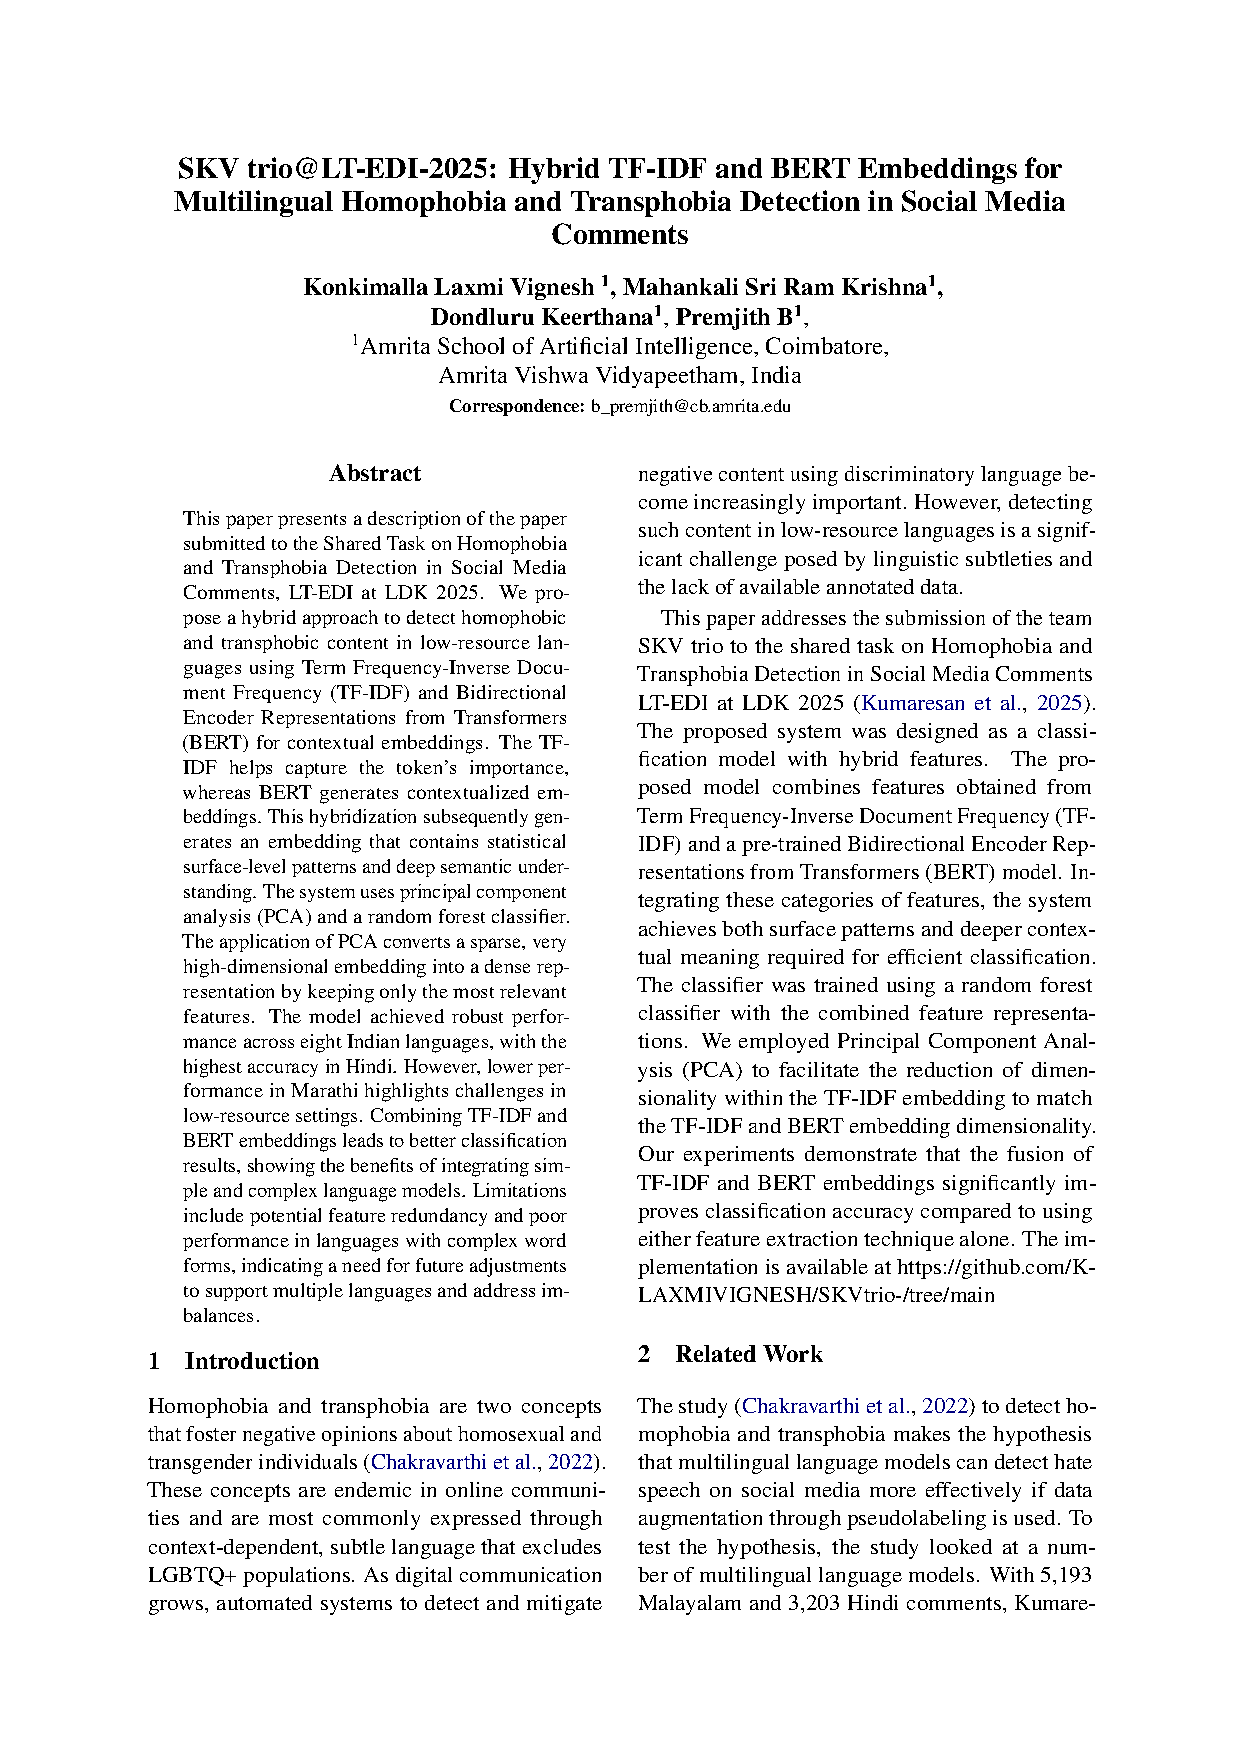
\includepdf[pagecommand={\thispagestyle{plain}},pages=-,addtotoc={1,section,1,{SKVtrio@LT-EDI-2025: Hybrid TF-IDF and BERT Embeddings for  Multilingual Homophobia and Transphobia Detection in Social Media  Comments},ref:paper_{6}}]{LT-EDI-2025/papers/6.pdf}
  \AddToShipoutPicture*{
    \setlength{\unitlength}{1mm}
    \footnotesize

            
    \put(0,13){\parbox[t]{\paperwidth}{\centering
    							\emph{Proceedings of the Fifth Workshop on Language Technology for Equality, Diversity, Inclusion}, pages 31--38 \\
  	  						September 9, 2025 \textcopyright
  							2025 Association for Computational Linguistics}}
  }
  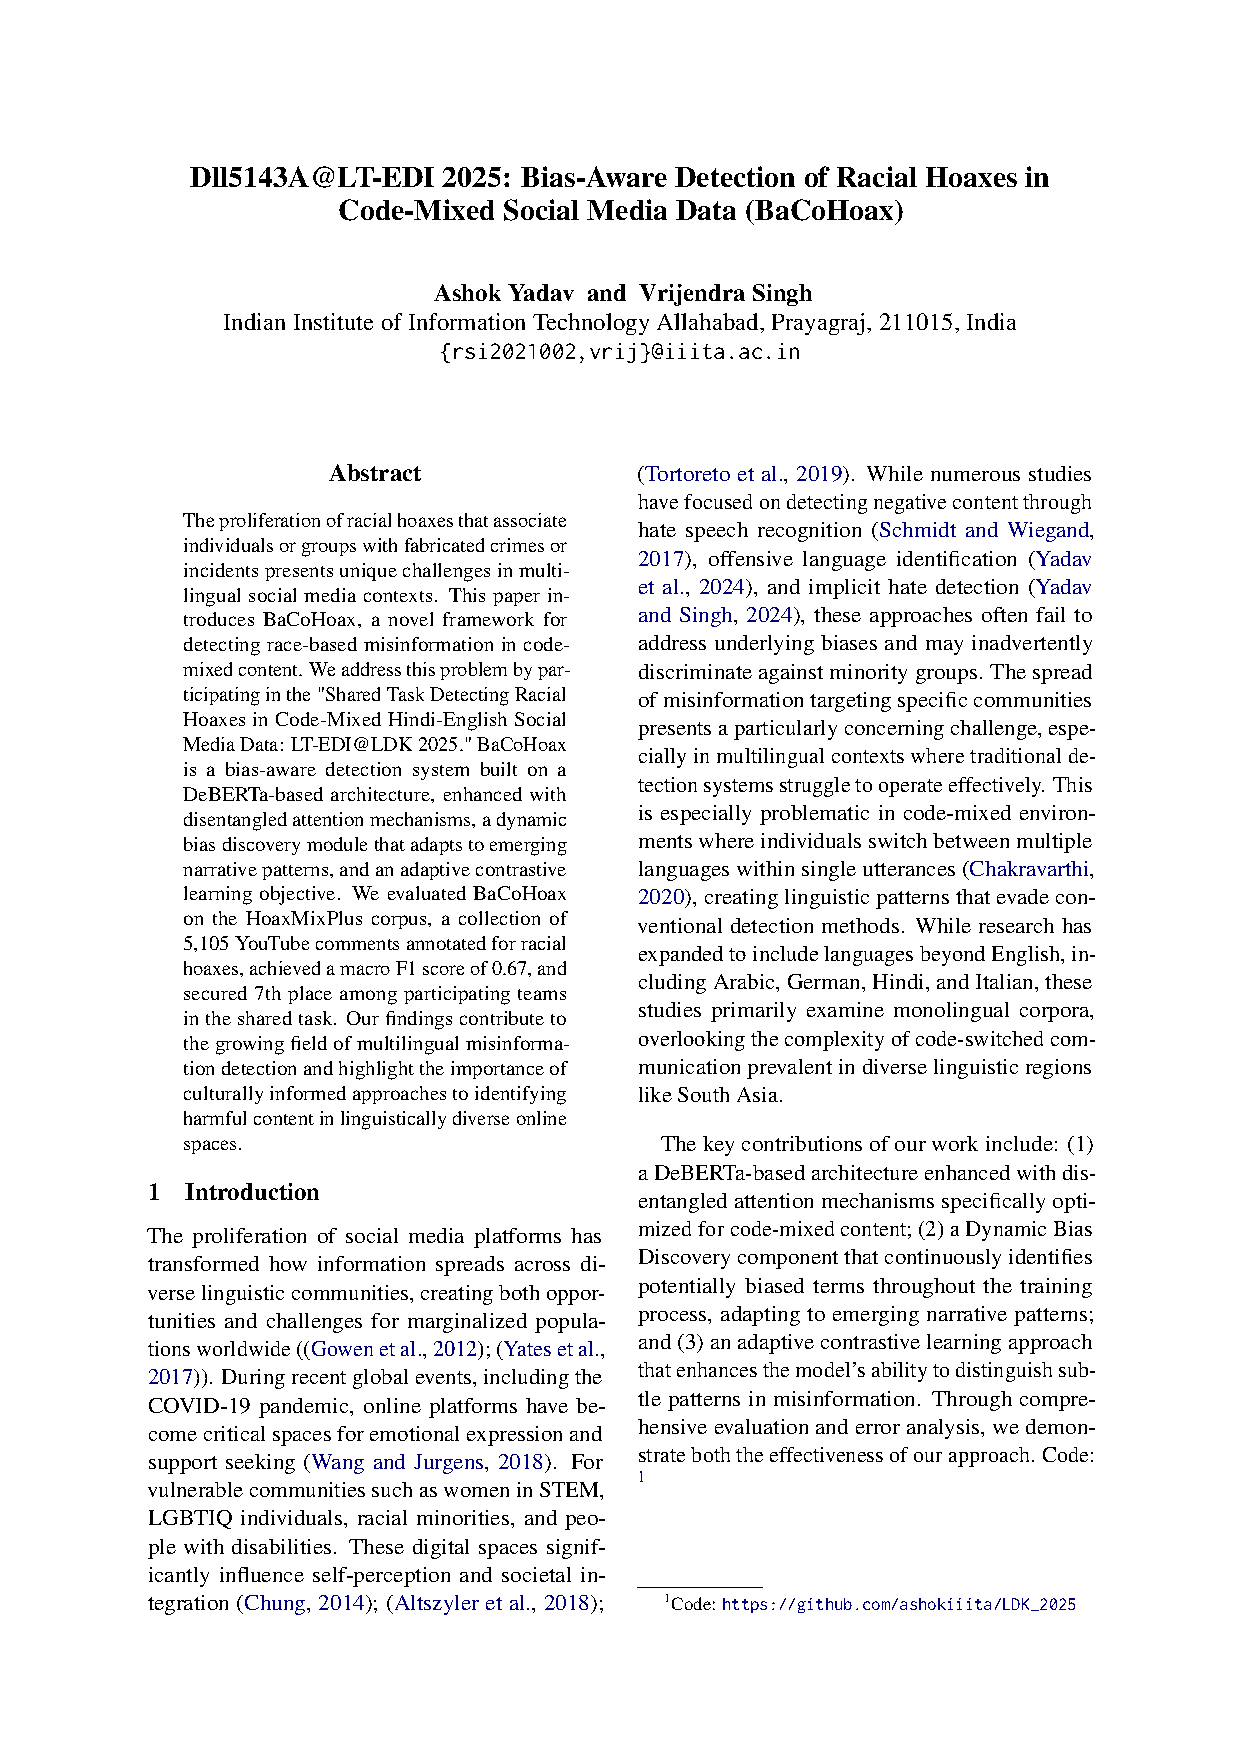
\includepdf[pagecommand={\thispagestyle{plain}},pages=-,addtotoc={1,section,1,{Dll5143A@LT-EDI 2025: Bias-Aware Detection of Racial Hoaxes in Code-Mixed Social Media Data (BaCoHoax)},ref:paper_{8}}]{LT-EDI-2025/papers/8.pdf}
  \AddToShipoutPicture*{
    \setlength{\unitlength}{1mm}
    \footnotesize

            
    \put(0,13){\parbox[t]{\paperwidth}{\centering
    							\emph{Proceedings of the Fifth Workshop on Language Technology for Equality, Diversity, Inclusion}, pages 39--46 \\
  	  						September 9, 2025 \textcopyright
  							2025 Association for Computational Linguistics}}
  }
  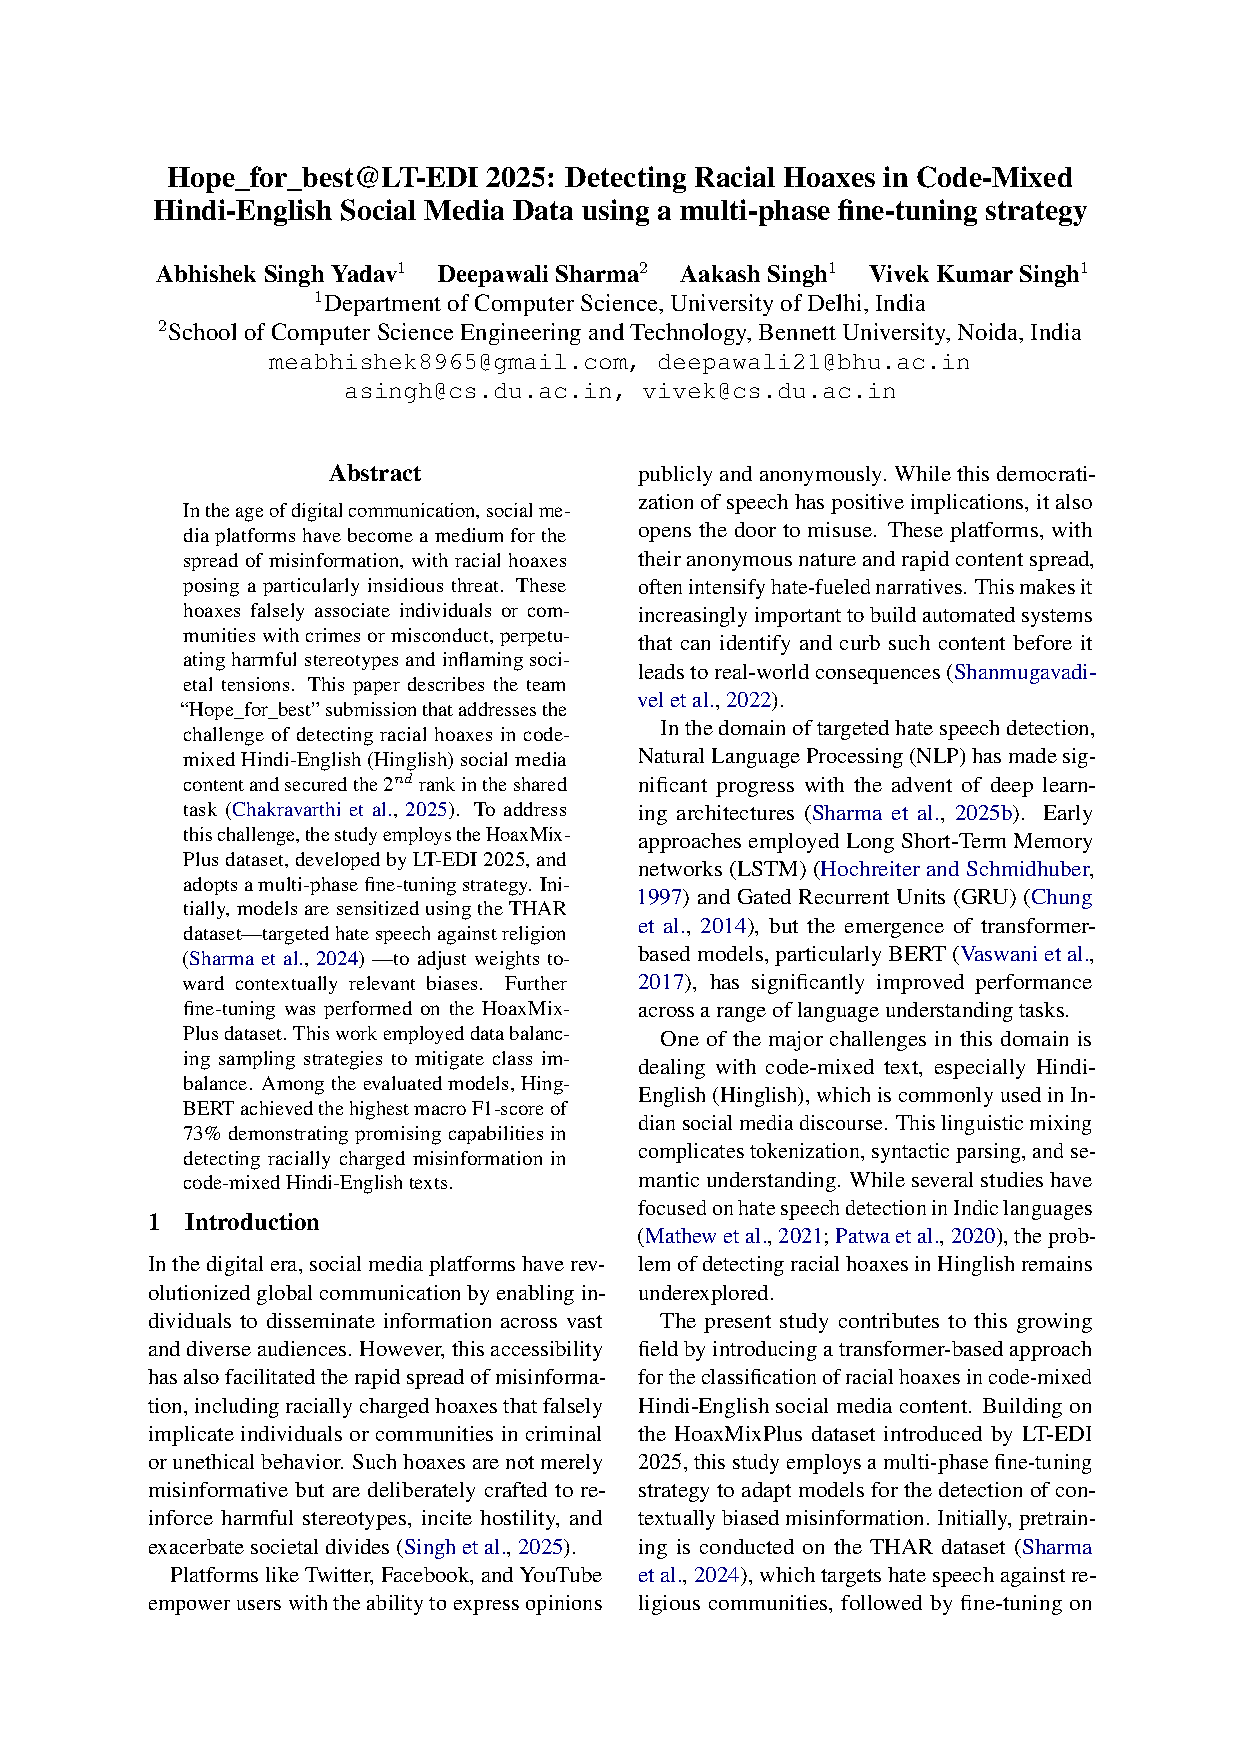
\includepdf[pagecommand={\thispagestyle{plain}},pages=-,addtotoc={1,section,1,{Hope\_for\_best@LT-EDI 2025: Detecting Racial Hoaxes in Code-Mixed Hindi-English Social Media Data using a multi-phase fine-tuning strategy},ref:paper_{9}}]{LT-EDI-2025/papers/9.pdf}
  \AddToShipoutPicture*{
    \setlength{\unitlength}{1mm}
    \footnotesize

            
    \put(0,13){\parbox[t]{\paperwidth}{\centering
    							\emph{Proceedings of the Fifth Workshop on Language Technology for Equality, Diversity, Inclusion}, pages 47--53 \\
  	  						September 9, 2025 \textcopyright
  							2025 Association for Computational Linguistics}}
  }
  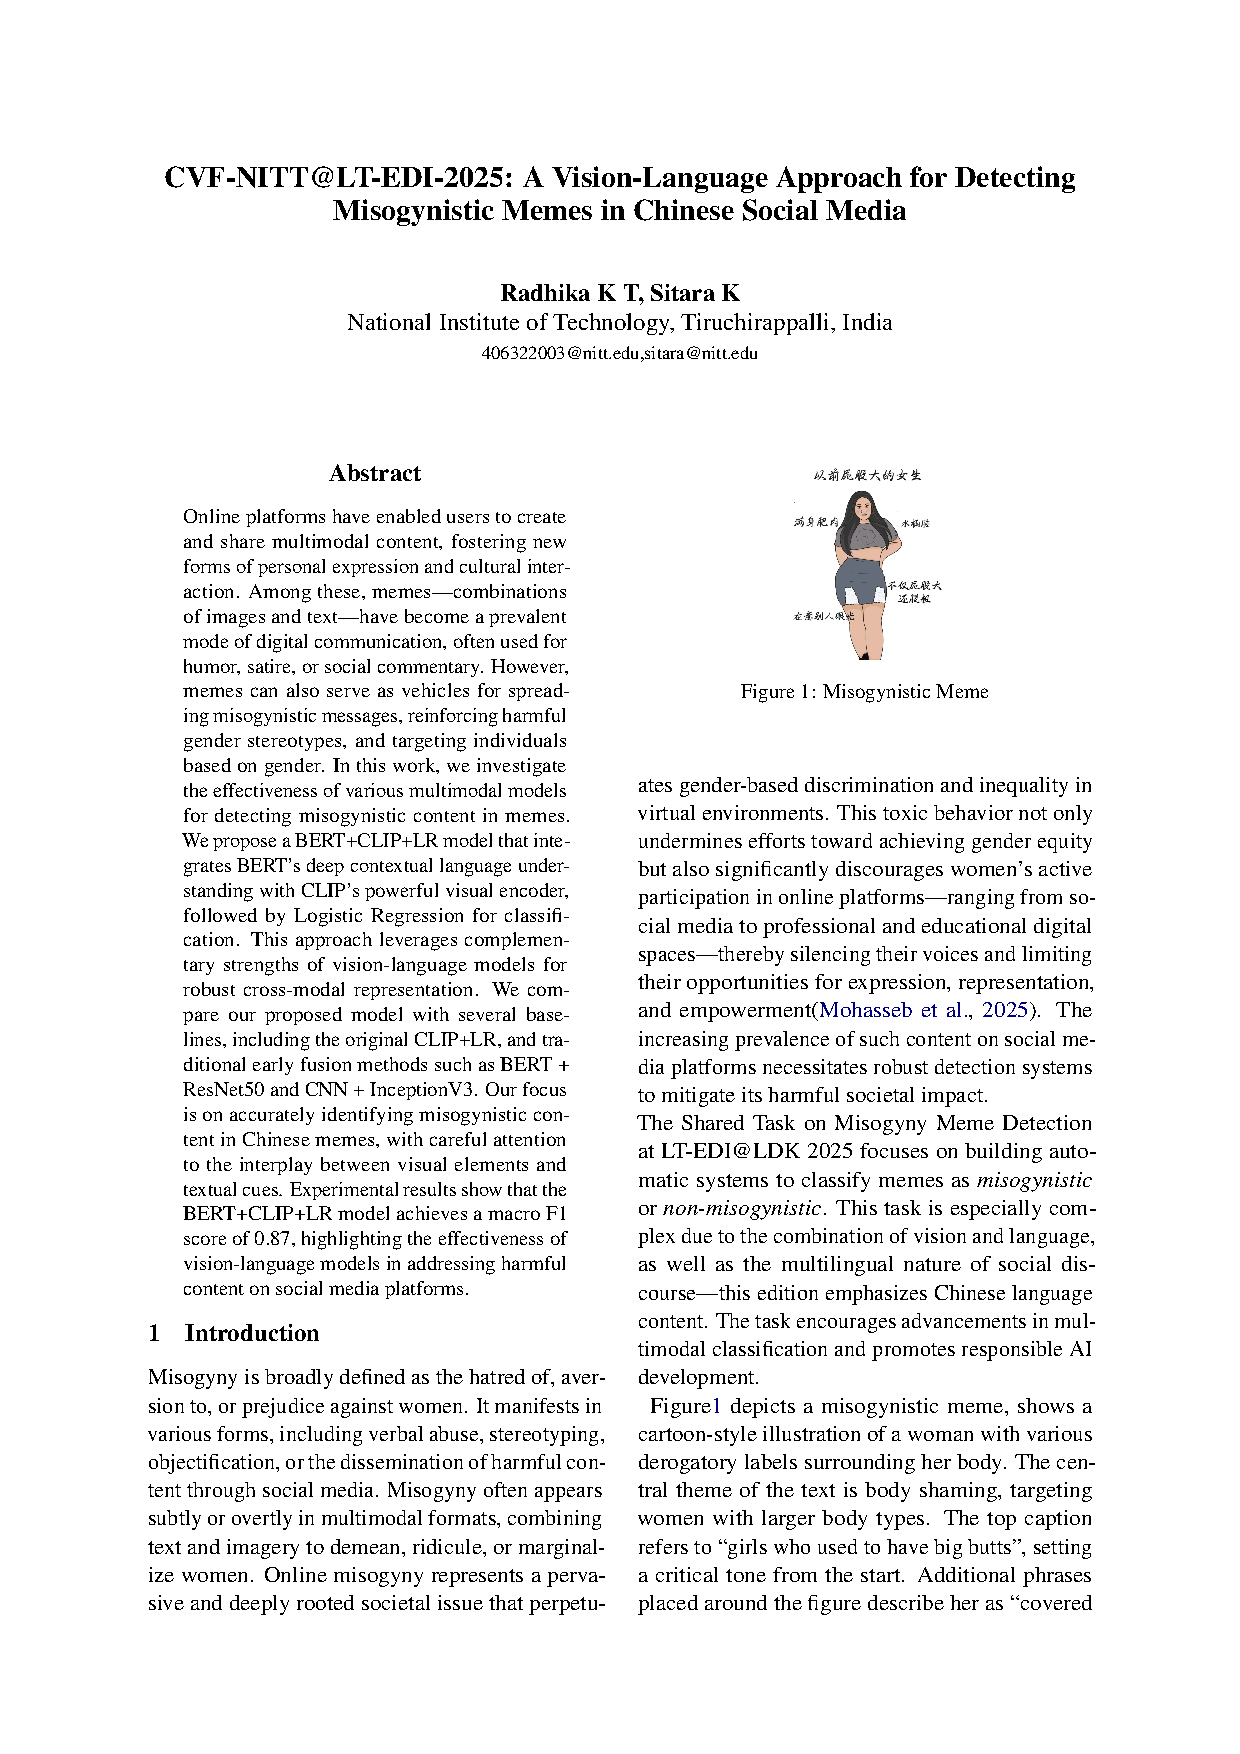
\includepdf[pagecommand={\thispagestyle{plain}},pages=-,addtotoc={1,section,1,{CVF-NITT@LT-EDI-2025:MisogynyDetection},ref:paper_{10}}]{LT-EDI-2025/papers/10.pdf}
  \AddToShipoutPicture*{
    \setlength{\unitlength}{1mm}
    \footnotesize

            
    \put(0,13){\parbox[t]{\paperwidth}{\centering
    							\emph{Proceedings of the Fifth Workshop on Language Technology for Equality, Diversity, Inclusion}, pages 54--62 \\
  	  						September 9, 2025 \textcopyright
  							2025 Association for Computational Linguistics}}
  }
  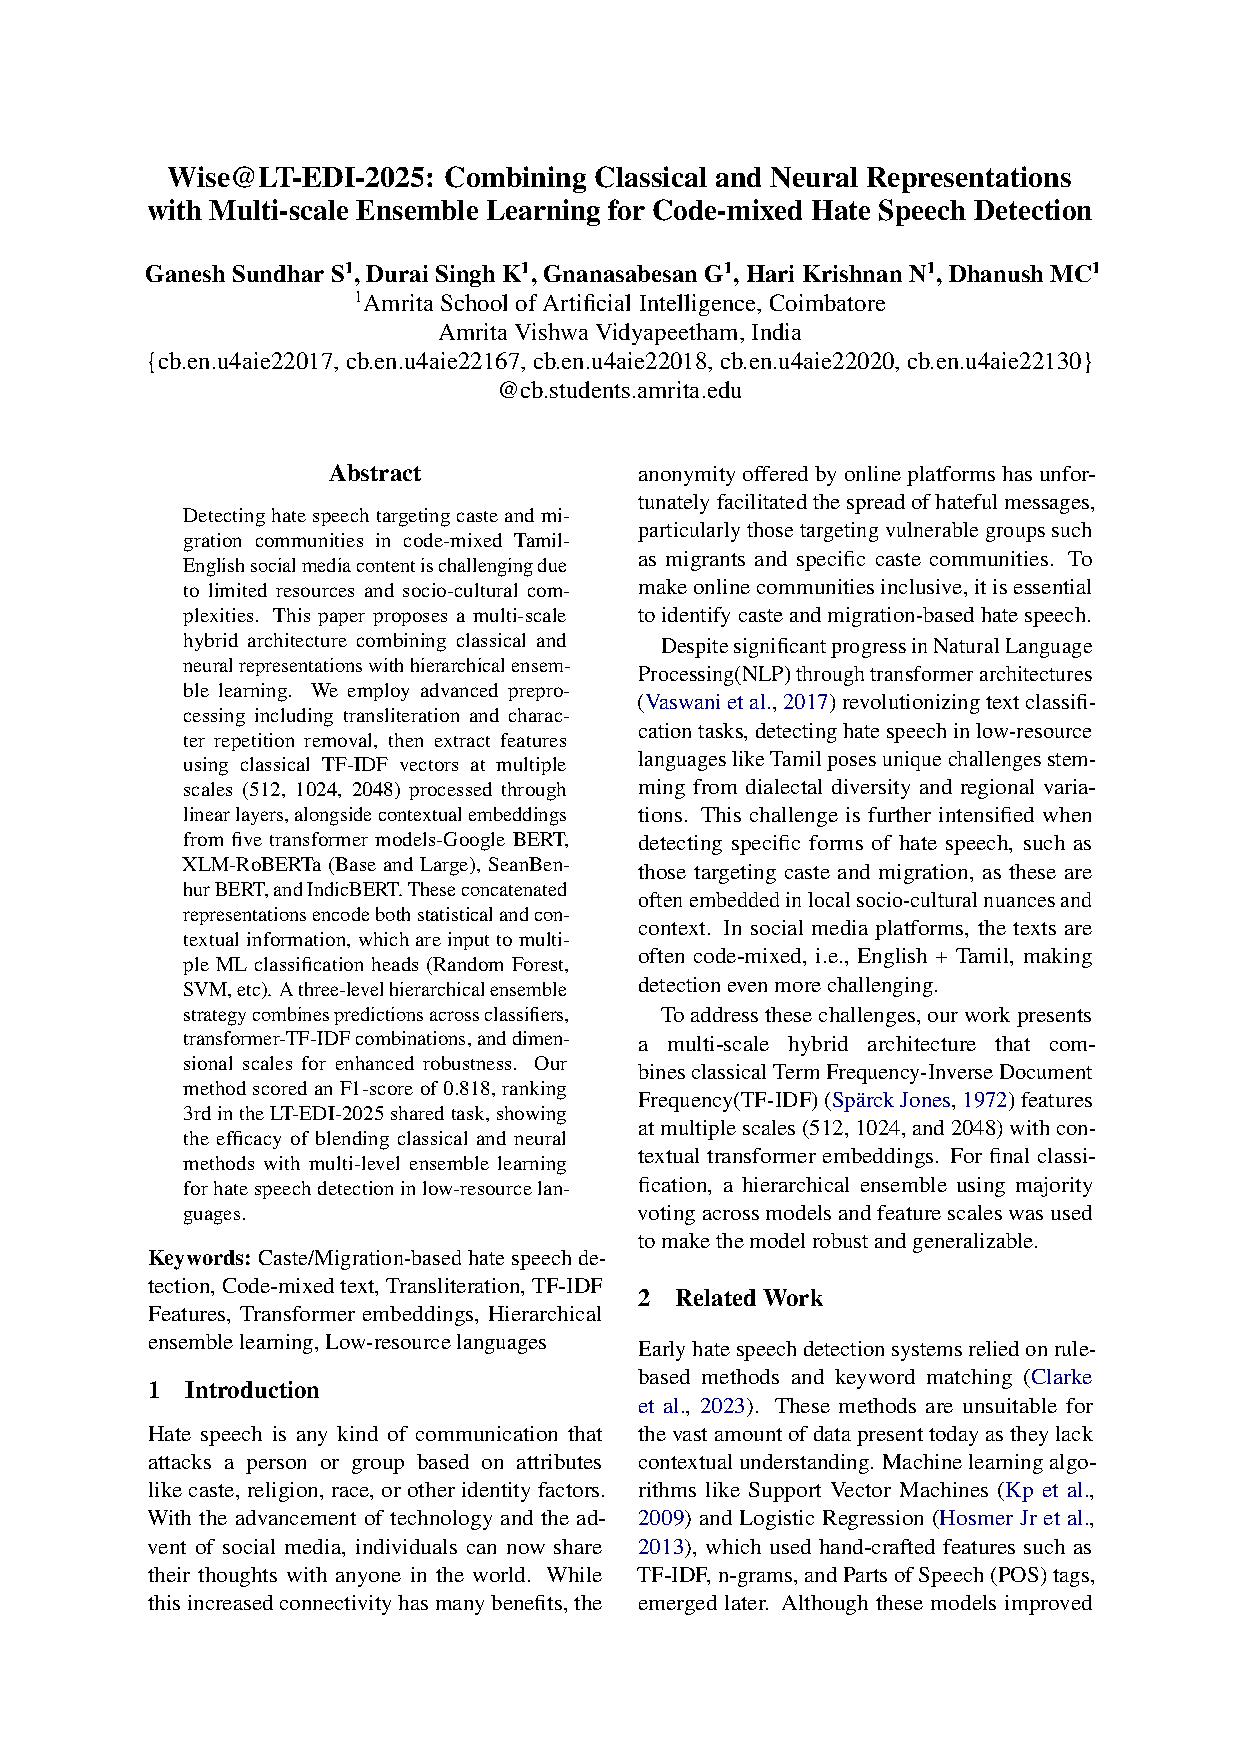
\includepdf[pagecommand={\thispagestyle{plain}},pages=-,addtotoc={1,section,1,{Wise@LT-EDI-2025: Combining Classical and Neural Representations with Multi-scale Ensemble Learning for Code-mixed Hate Speech Detection},ref:paper_{11}}]{LT-EDI-2025/papers/11.pdf}
  \AddToShipoutPicture*{
    \setlength{\unitlength}{1mm}
    \footnotesize

            
    \put(0,13){\parbox[t]{\paperwidth}{\centering
    							\emph{Proceedings of the Fifth Workshop on Language Technology for Equality, Diversity, Inclusion}, pages 63--67 \\
  	  						September 9, 2025 \textcopyright
  							2025 Association for Computational Linguistics}}
  }
  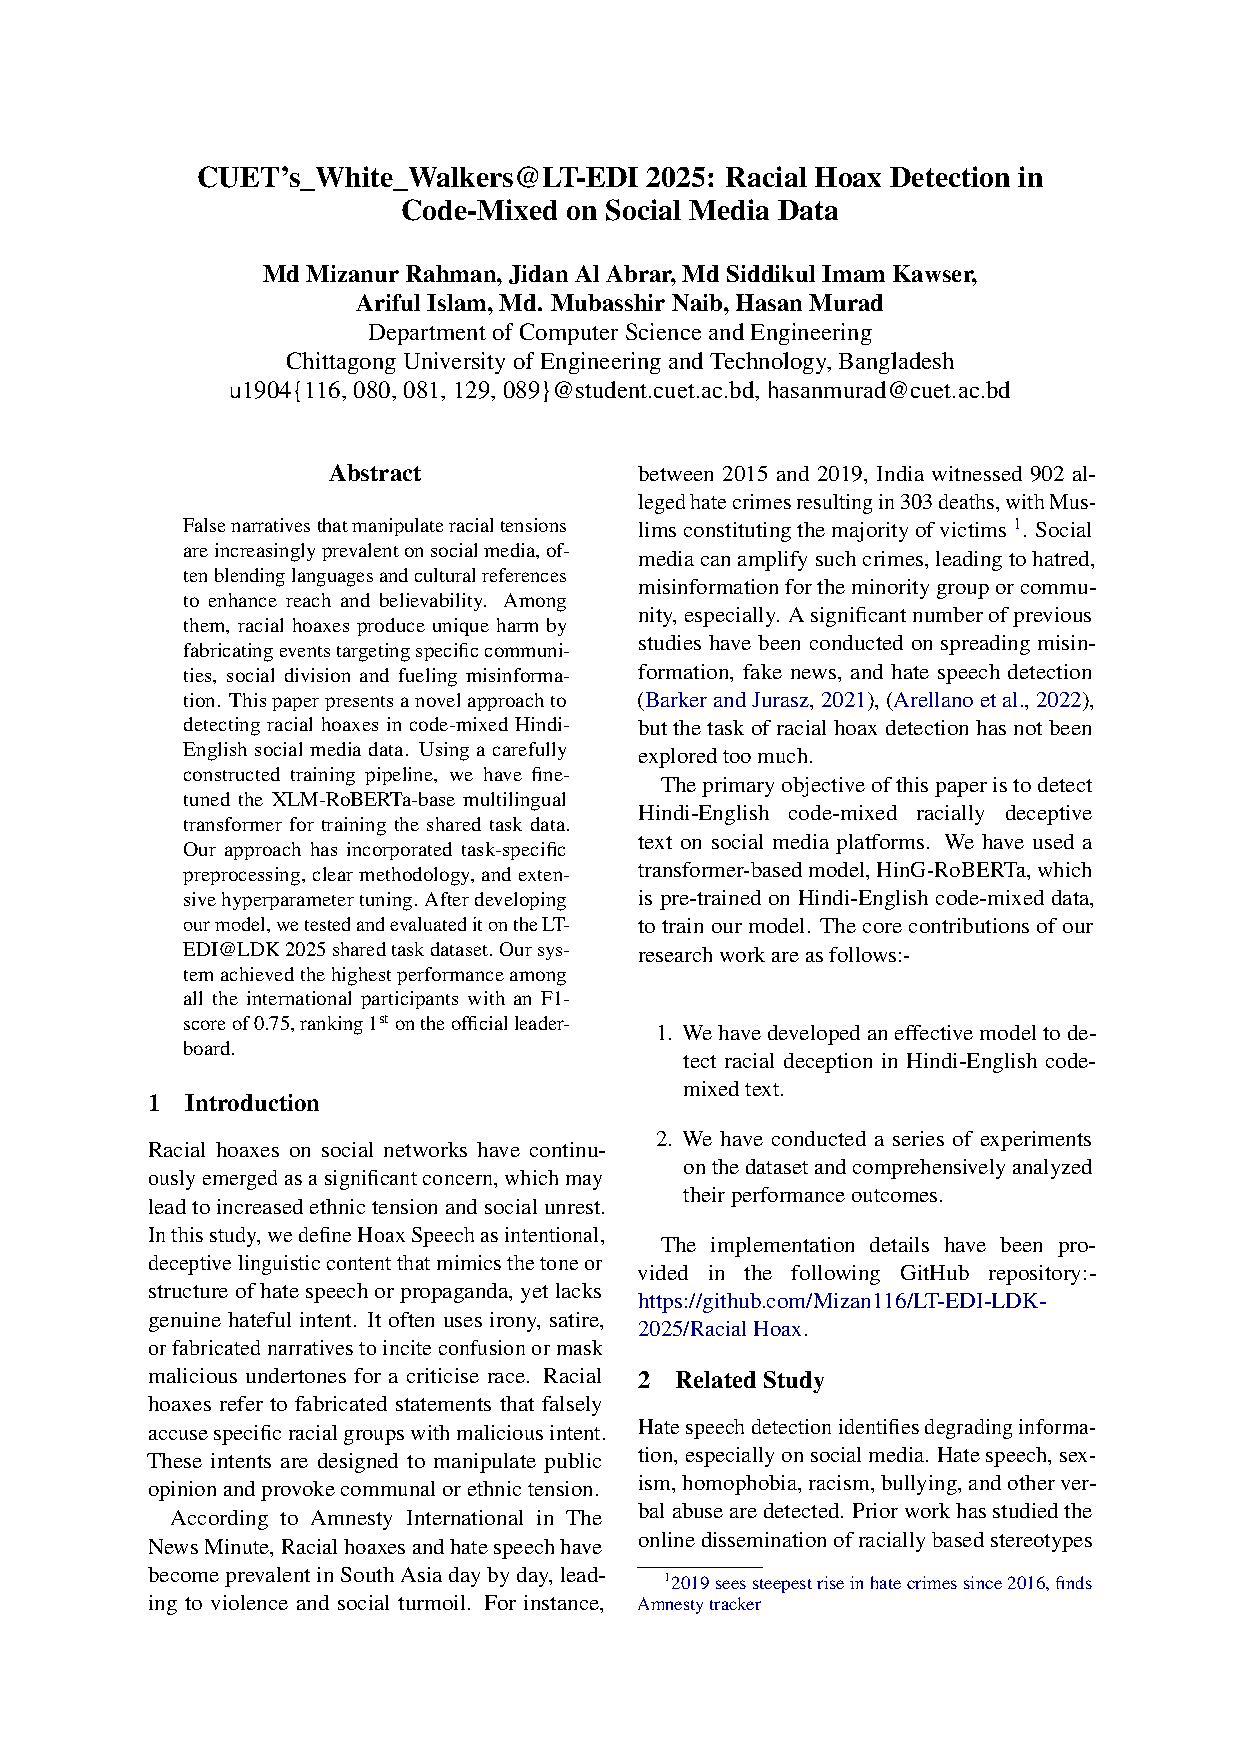
\includepdf[pagecommand={\thispagestyle{plain}},pages=-,addtotoc={1,section,1,{CUET's\_White\_Walkers@LT-EDI 2025: Racial Hoax Detection in Code-Mixed on Social Media Data},ref:paper_{13}}]{LT-EDI-2025/papers/13.pdf}
  \AddToShipoutPicture*{
    \setlength{\unitlength}{1mm}
    \footnotesize

            
    \put(0,13){\parbox[t]{\paperwidth}{\centering
    							\emph{Proceedings of the Fifth Workshop on Language Technology for Equality, Diversity, Inclusion}, pages 68--74 \\
  	  						September 9, 2025 \textcopyright
  							2025 Association for Computational Linguistics}}
  }
  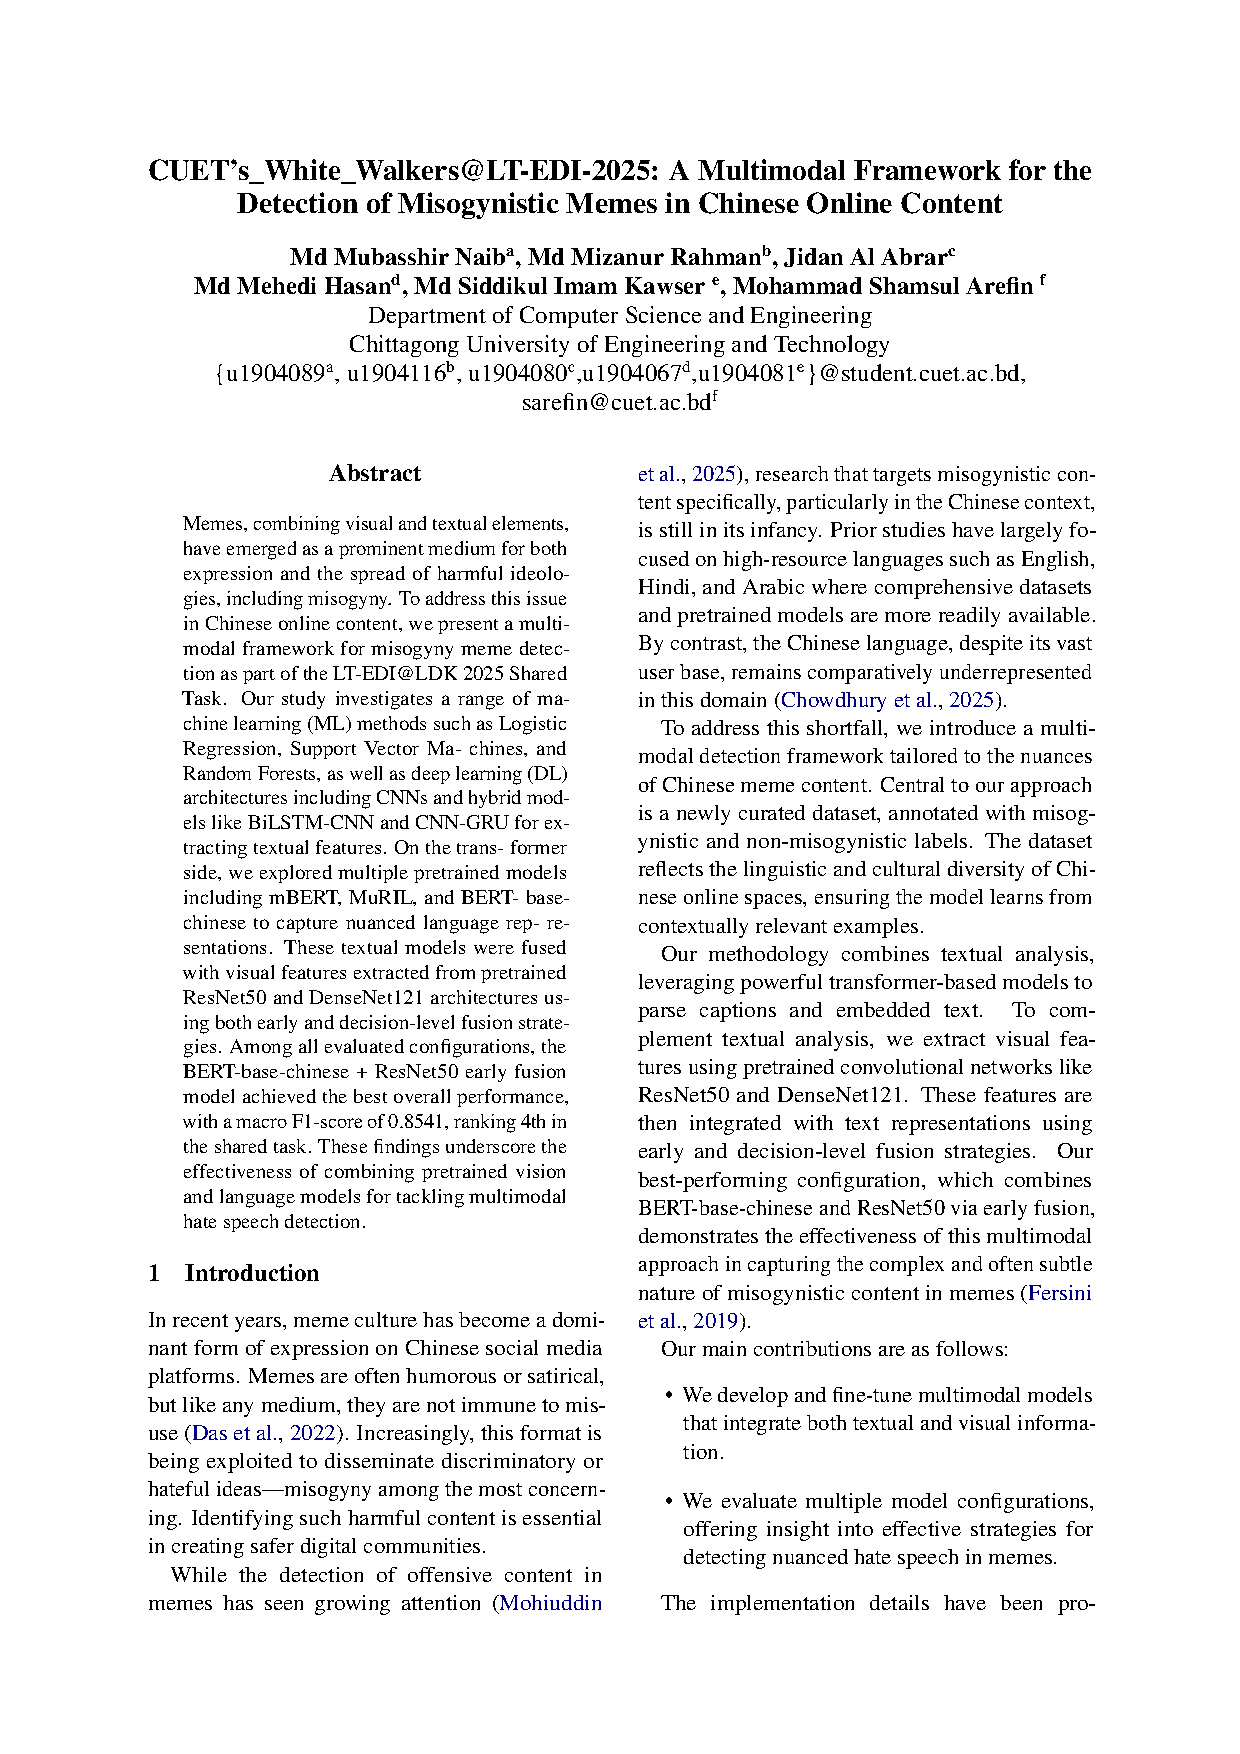
\includepdf[pagecommand={\thispagestyle{plain}},pages=-,addtotoc={1,section,1,{CUET's\_White\_Walkers@LT-EDI-2025: A Multimodal Framework for the Detection of Misogynistic Memes in Chinese Online Content},ref:paper_{14}}]{LT-EDI-2025/papers/14.pdf}
  \AddToShipoutPicture*{
    \setlength{\unitlength}{1mm}
    \footnotesize

            
    \put(0,13){\parbox[t]{\paperwidth}{\centering
    							\emph{Proceedings of the Fifth Workshop on Language Technology for Equality, Diversity, Inclusion}, pages 75--79 \\
  	  						September 9, 2025 \textcopyright
  							2025 Association for Computational Linguistics}}
  }
  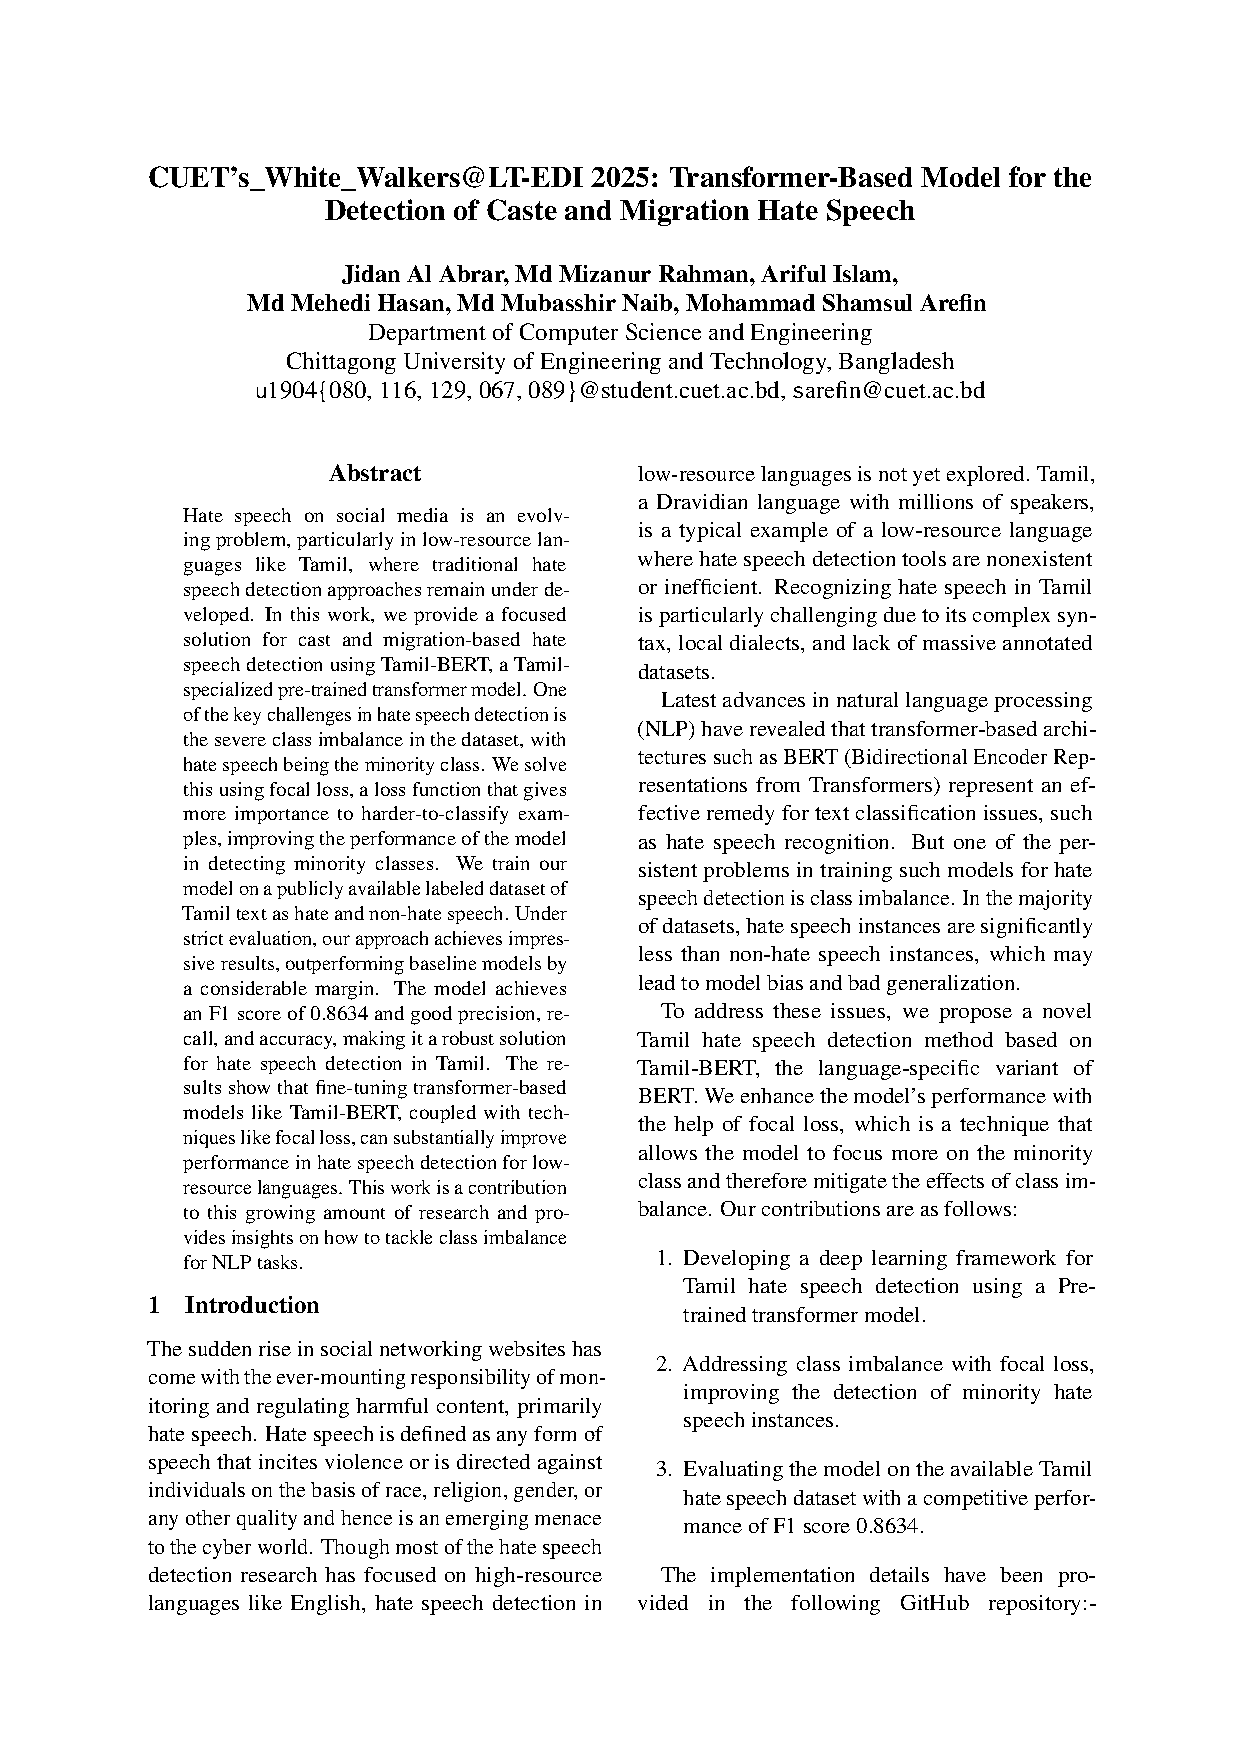
\includepdf[pagecommand={\thispagestyle{plain}},pages=-,addtotoc={1,section,1,{CUET's\_White\_Walkers@LT-EDI 2025: Transformer-Based Model for the Detection of Caste and Migration Hate Speech},ref:paper_{15}}]{LT-EDI-2025/papers/15.pdf}
  \AddToShipoutPicture*{
    \setlength{\unitlength}{1mm}
    \footnotesize

            
    \put(0,13){\parbox[t]{\paperwidth}{\centering
    							\emph{Proceedings of the Fifth Workshop on Language Technology for Equality, Diversity, Inclusion}, pages 80--83 \\
  	  						September 9, 2025 \textcopyright
  							2025 Association for Computational Linguistics}}
  }
  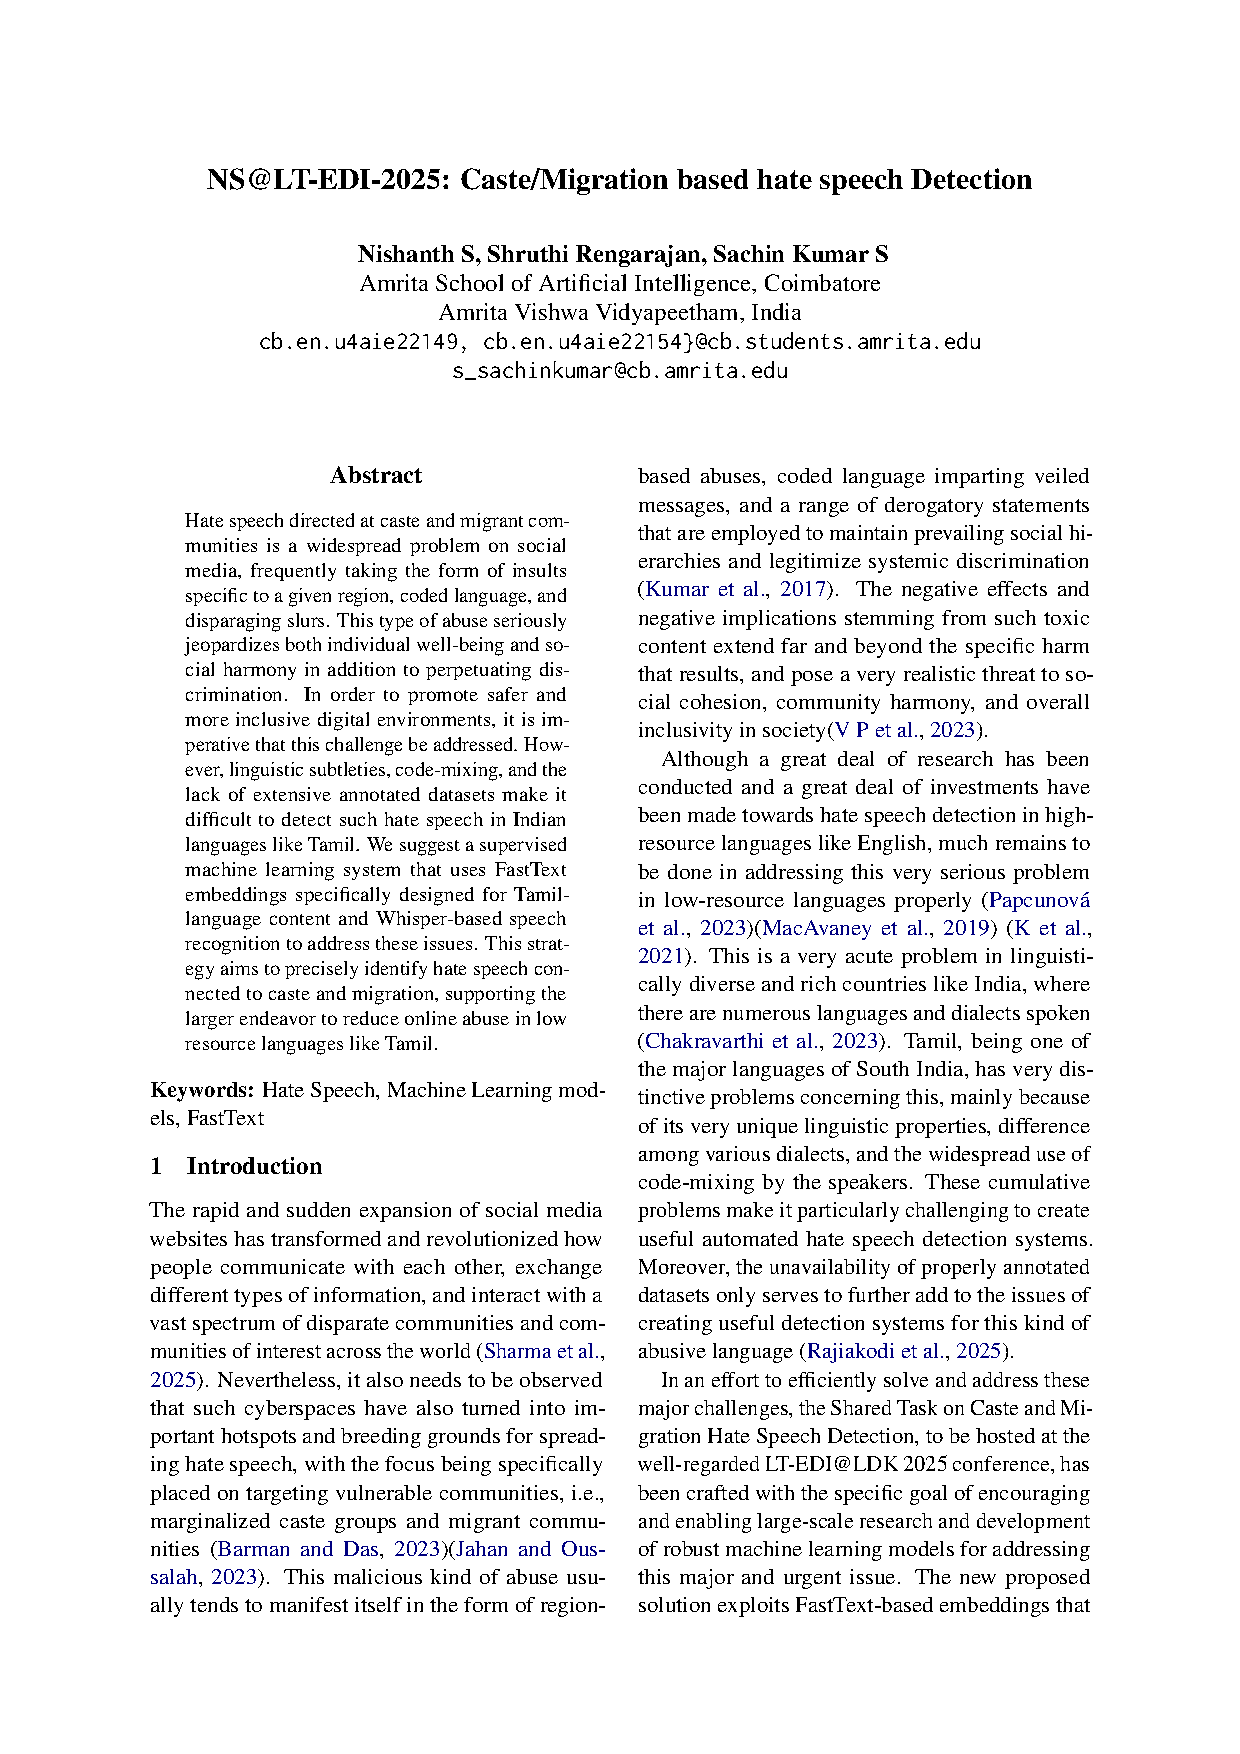
\includepdf[pagecommand={\thispagestyle{plain}},pages=-,addtotoc={1,section,1,{NS@LT-EDI-2025 CasteMigration based hate speech Detection},ref:paper_{16}}]{LT-EDI-2025/papers/16.pdf}
  \AddToShipoutPicture*{
    \setlength{\unitlength}{1mm}
    \footnotesize

            
    \put(0,13){\parbox[t]{\paperwidth}{\centering
    							\emph{Proceedings of the Fifth Workshop on Language Technology for Equality, Diversity, Inclusion}, pages 84--89 \\
  	  						September 9, 2025 \textcopyright
  							2025 Association for Computational Linguistics}}
  }
  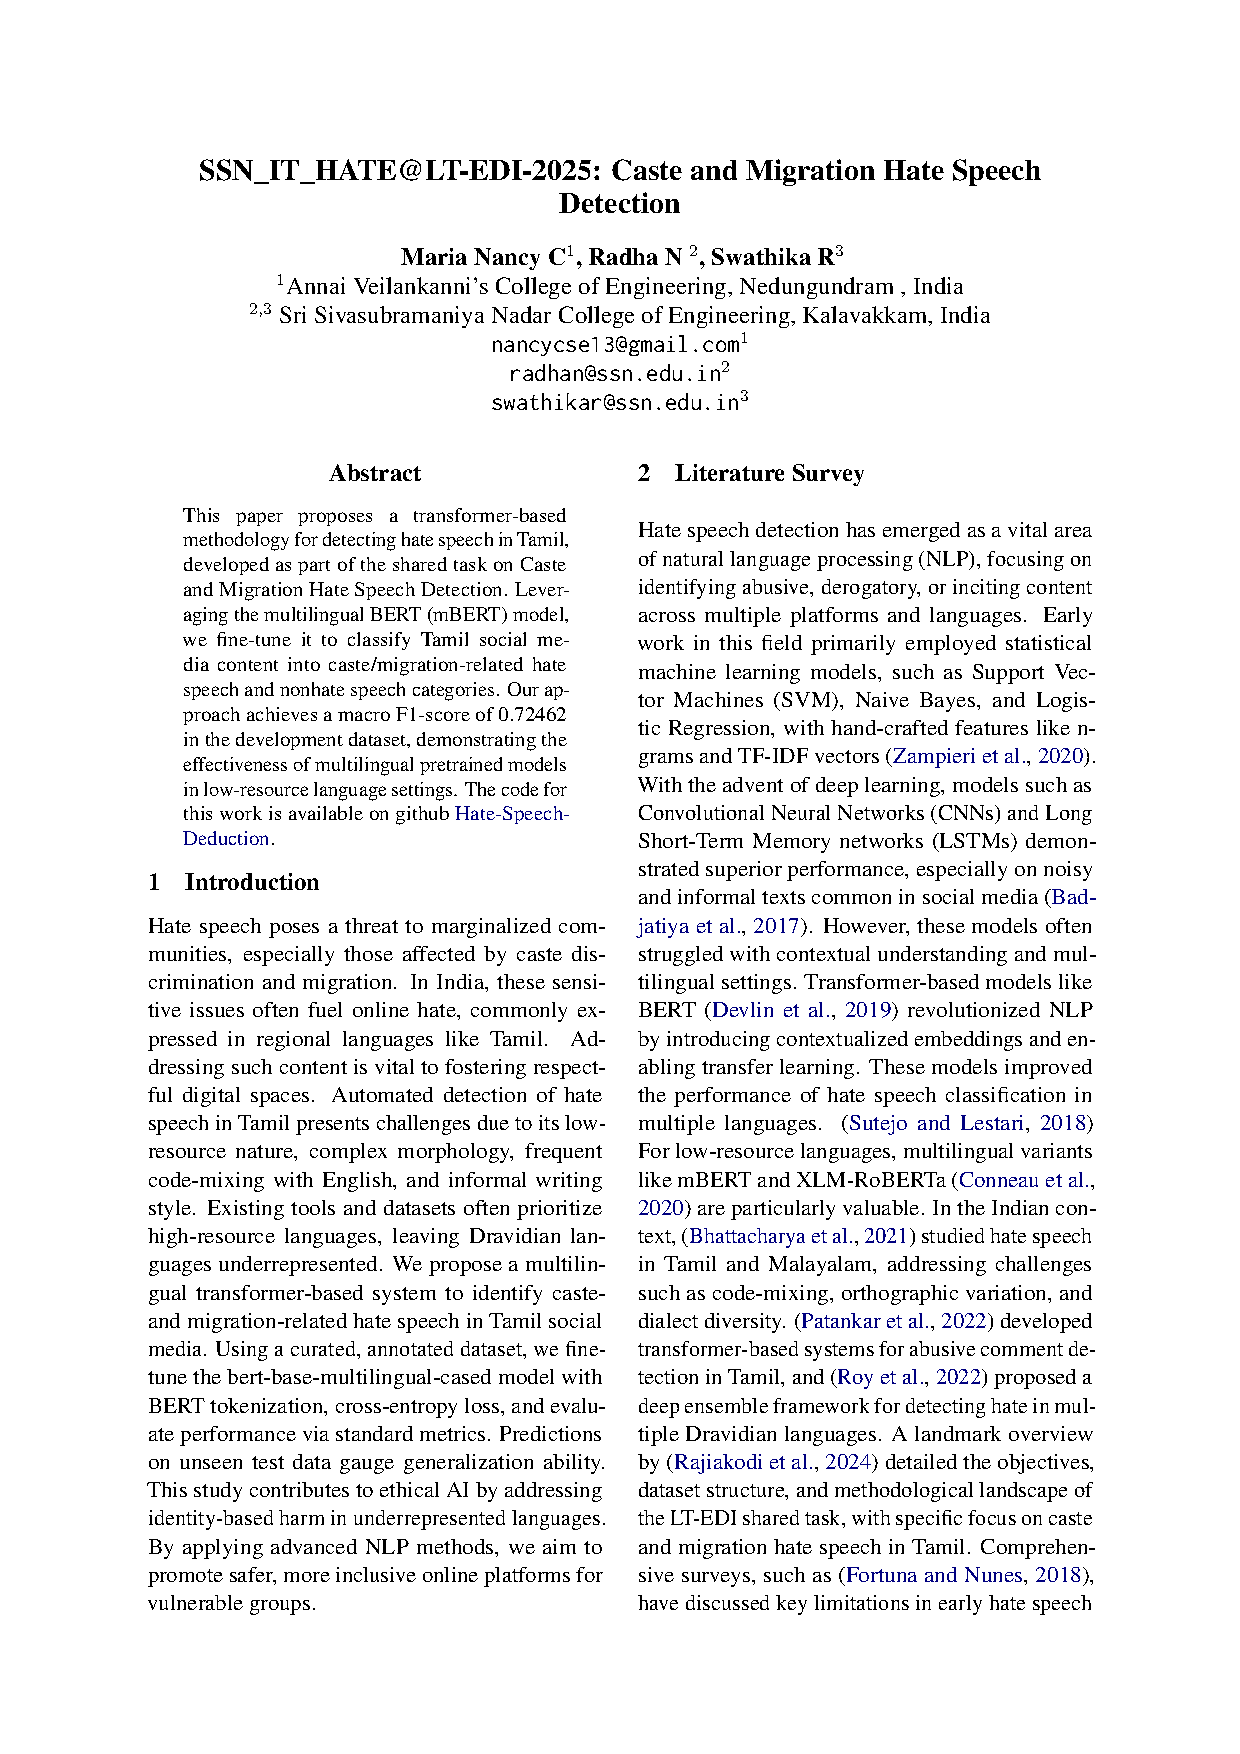
\includepdf[pagecommand={\thispagestyle{plain}},pages=-,addtotoc={1,section,1,{SSN\_IT\_HATE@LT-EDI-2025: Caste and Migration Hate Speech Detection},ref:paper_{17}}]{LT-EDI-2025/papers/17.pdf}
  \AddToShipoutPicture*{
    \setlength{\unitlength}{1mm}
    \footnotesize

            
    \put(0,13){\parbox[t]{\paperwidth}{\centering
    							\emph{Proceedings of the Fifth Workshop on Language Technology for Equality, Diversity, Inclusion}, pages 90--94 \\
  	  						September 9, 2025 \textcopyright
  							2025 Association for Computational Linguistics}}
  }
  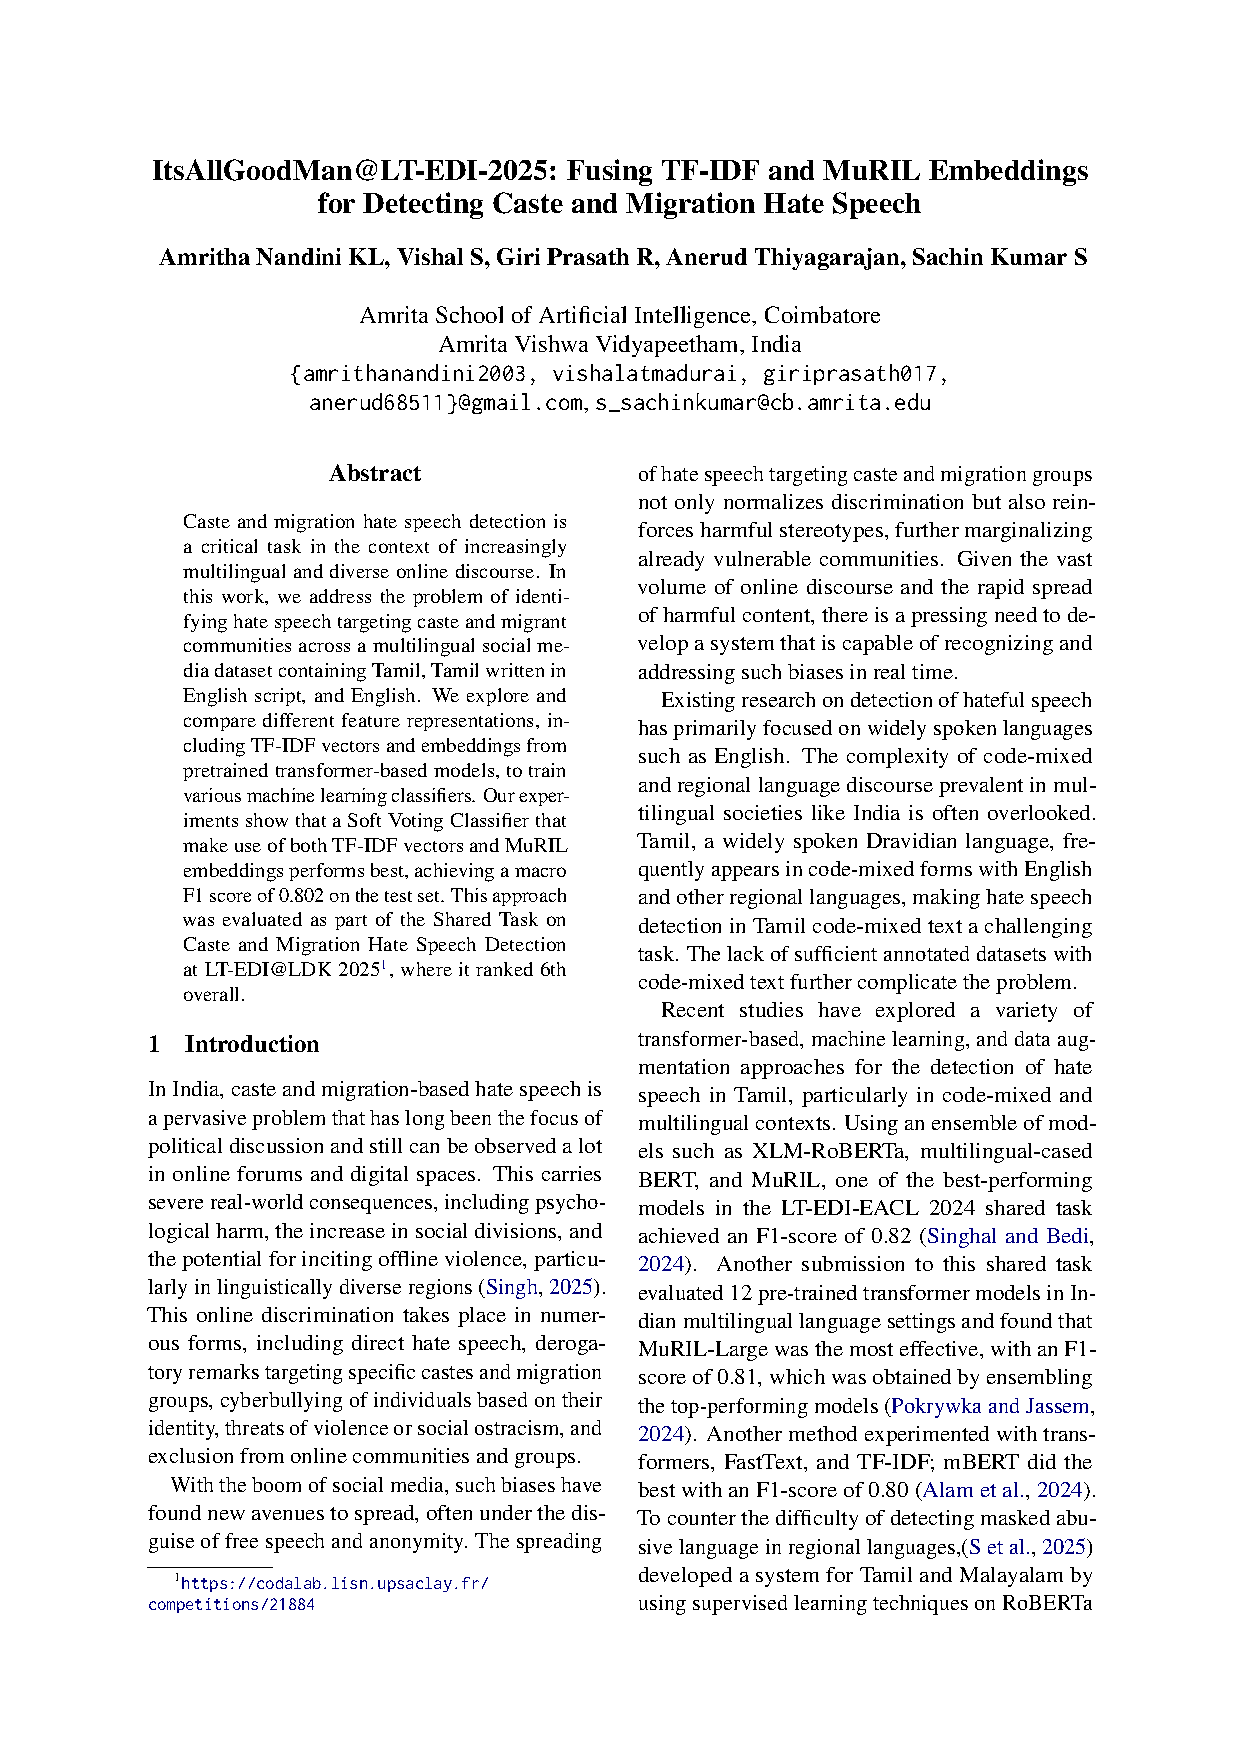
\includepdf[pagecommand={\thispagestyle{plain}},pages=-,addtotoc={1,section,1,{ItsAllGoodMan@LT-EDI-2025: Fusing TF-IDF and MuRIL Embeddings for Detecting Caste and Migration Hate Speech},ref:paper_{18}}]{LT-EDI-2025/papers/18.pdf}
  \AddToShipoutPicture*{
    \setlength{\unitlength}{1mm}
    \footnotesize

            
    \put(0,13){\parbox[t]{\paperwidth}{\centering
    							\emph{Proceedings of the Fifth Workshop on Language Technology for Equality, Diversity, Inclusion}, pages 95--99 \\
  	  						September 9, 2025 \textcopyright
  							2025 Association for Computational Linguistics}}
  }
  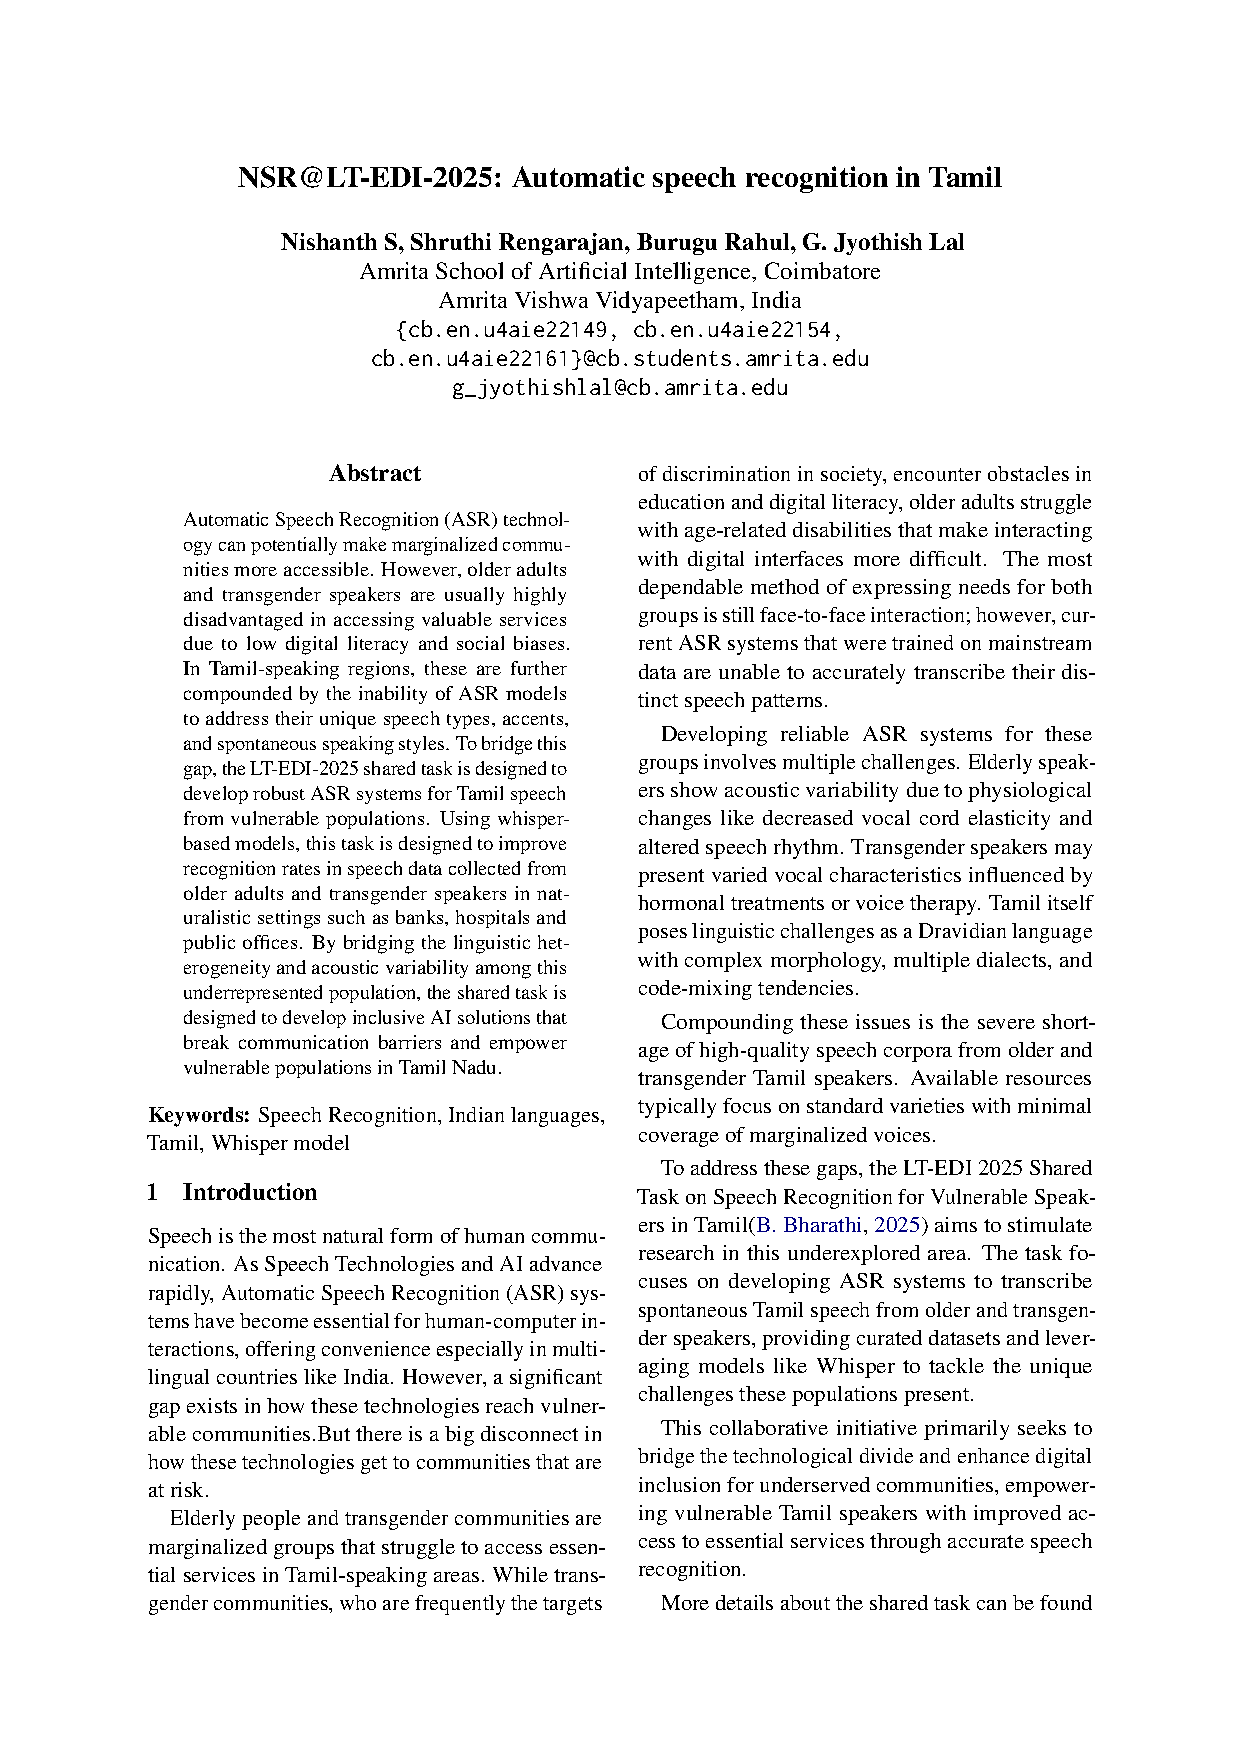
\includepdf[pagecommand={\thispagestyle{plain}},pages=-,addtotoc={1,section,1,{NSR\_LT-EDI-2025 Automatic speech recognition in Tamil},ref:paper_{19}}]{LT-EDI-2025/papers/19.pdf}
  \AddToShipoutPicture*{
    \setlength{\unitlength}{1mm}
    \footnotesize

            
    \put(0,13){\parbox[t]{\paperwidth}{\centering
    							\emph{Proceedings of the Fifth Workshop on Language Technology for Equality, Diversity, Inclusion}, pages 100--104 \\
  	  						September 9, 2025 \textcopyright
  							2025 Association for Computational Linguistics}}
  }
  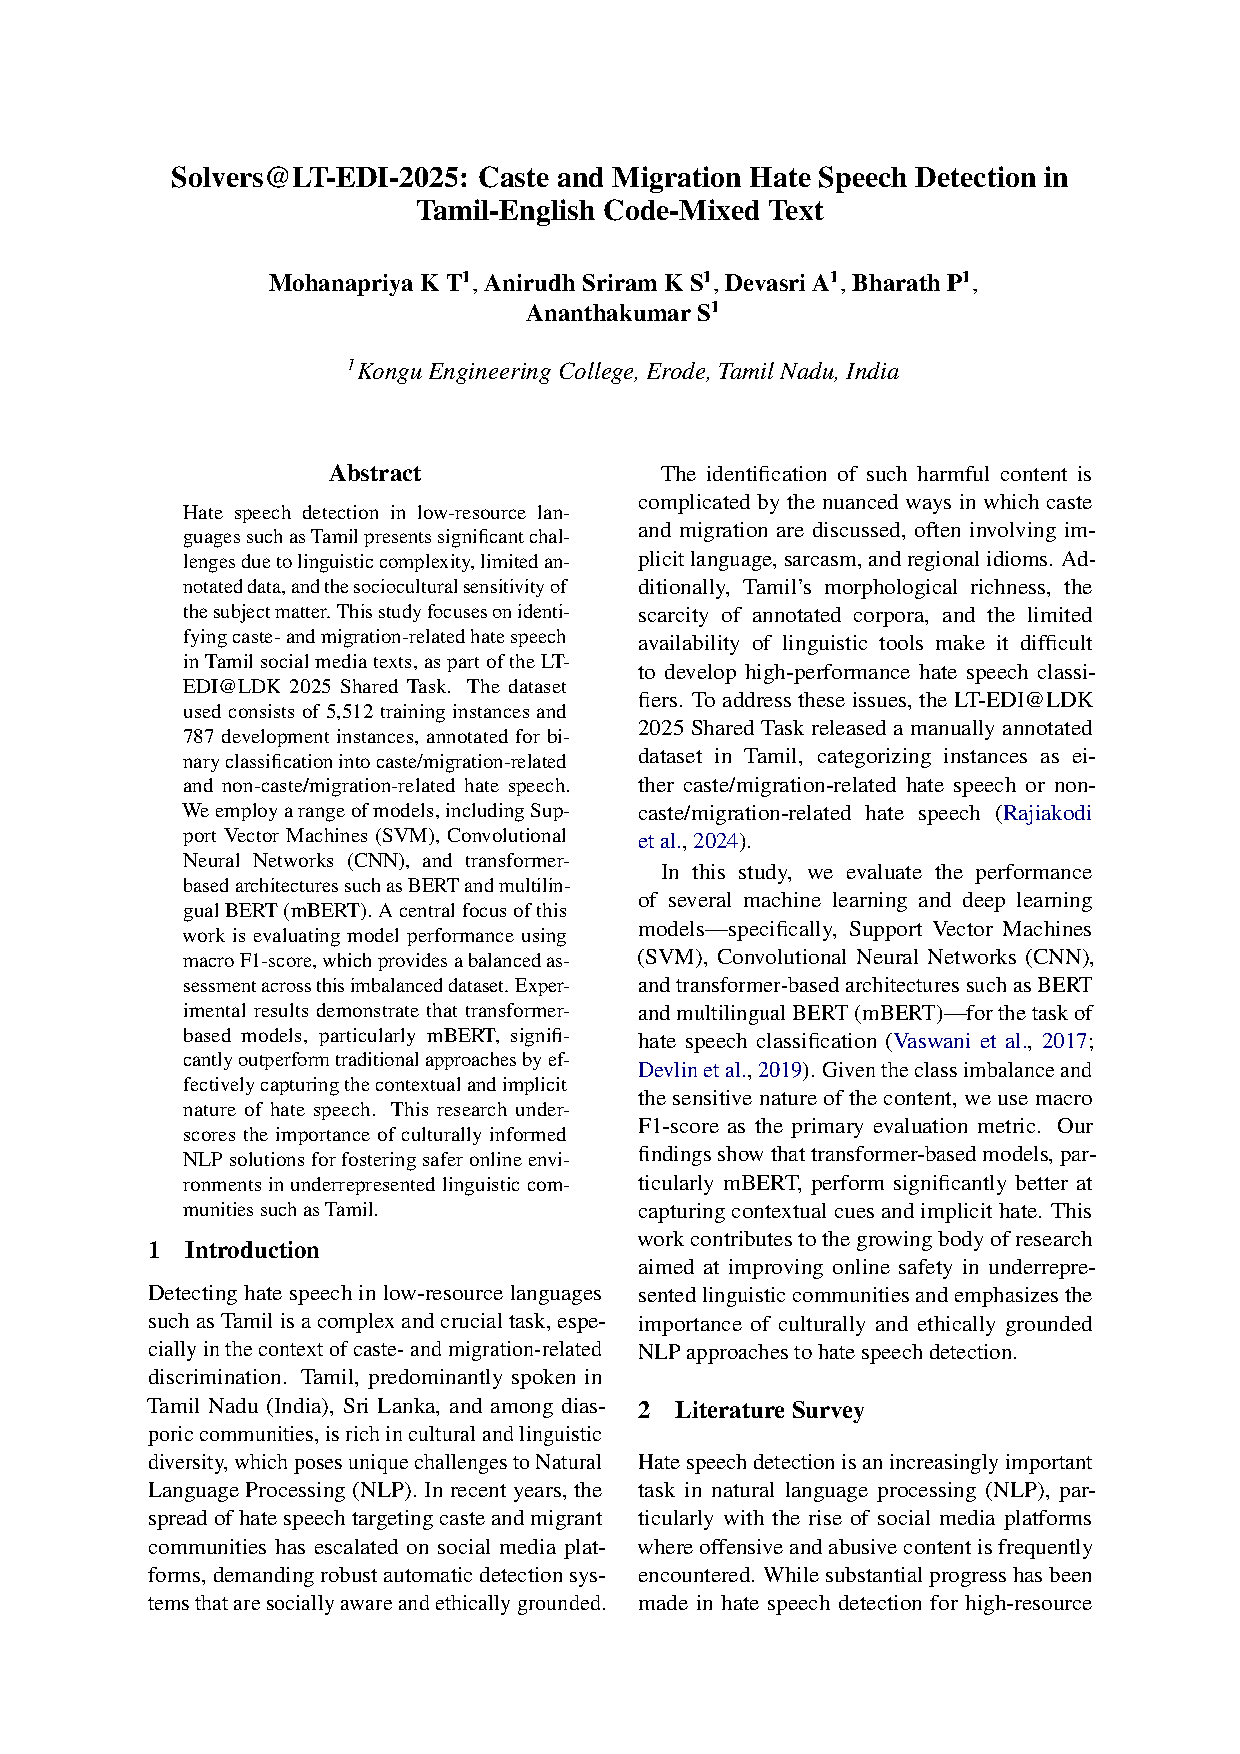
\includepdf[pagecommand={\thispagestyle{plain}},pages=-,addtotoc={1,section,1,{Solvers@LT-EDI-2025: Caste and Migration Hate Speech Detection in Tamil-English Code-Mixed Text},ref:paper_{20}}]{LT-EDI-2025/papers/20.pdf}
  \AddToShipoutPicture*{
    \setlength{\unitlength}{1mm}
    \footnotesize

            
    \put(0,13){\parbox[t]{\paperwidth}{\centering
    							\emph{Proceedings of the Fifth Workshop on Language Technology for Equality, Diversity, Inclusion}, pages 105--110 \\
  	  						September 9, 2025 \textcopyright
  							2025 Association for Computational Linguistics}}
  }
  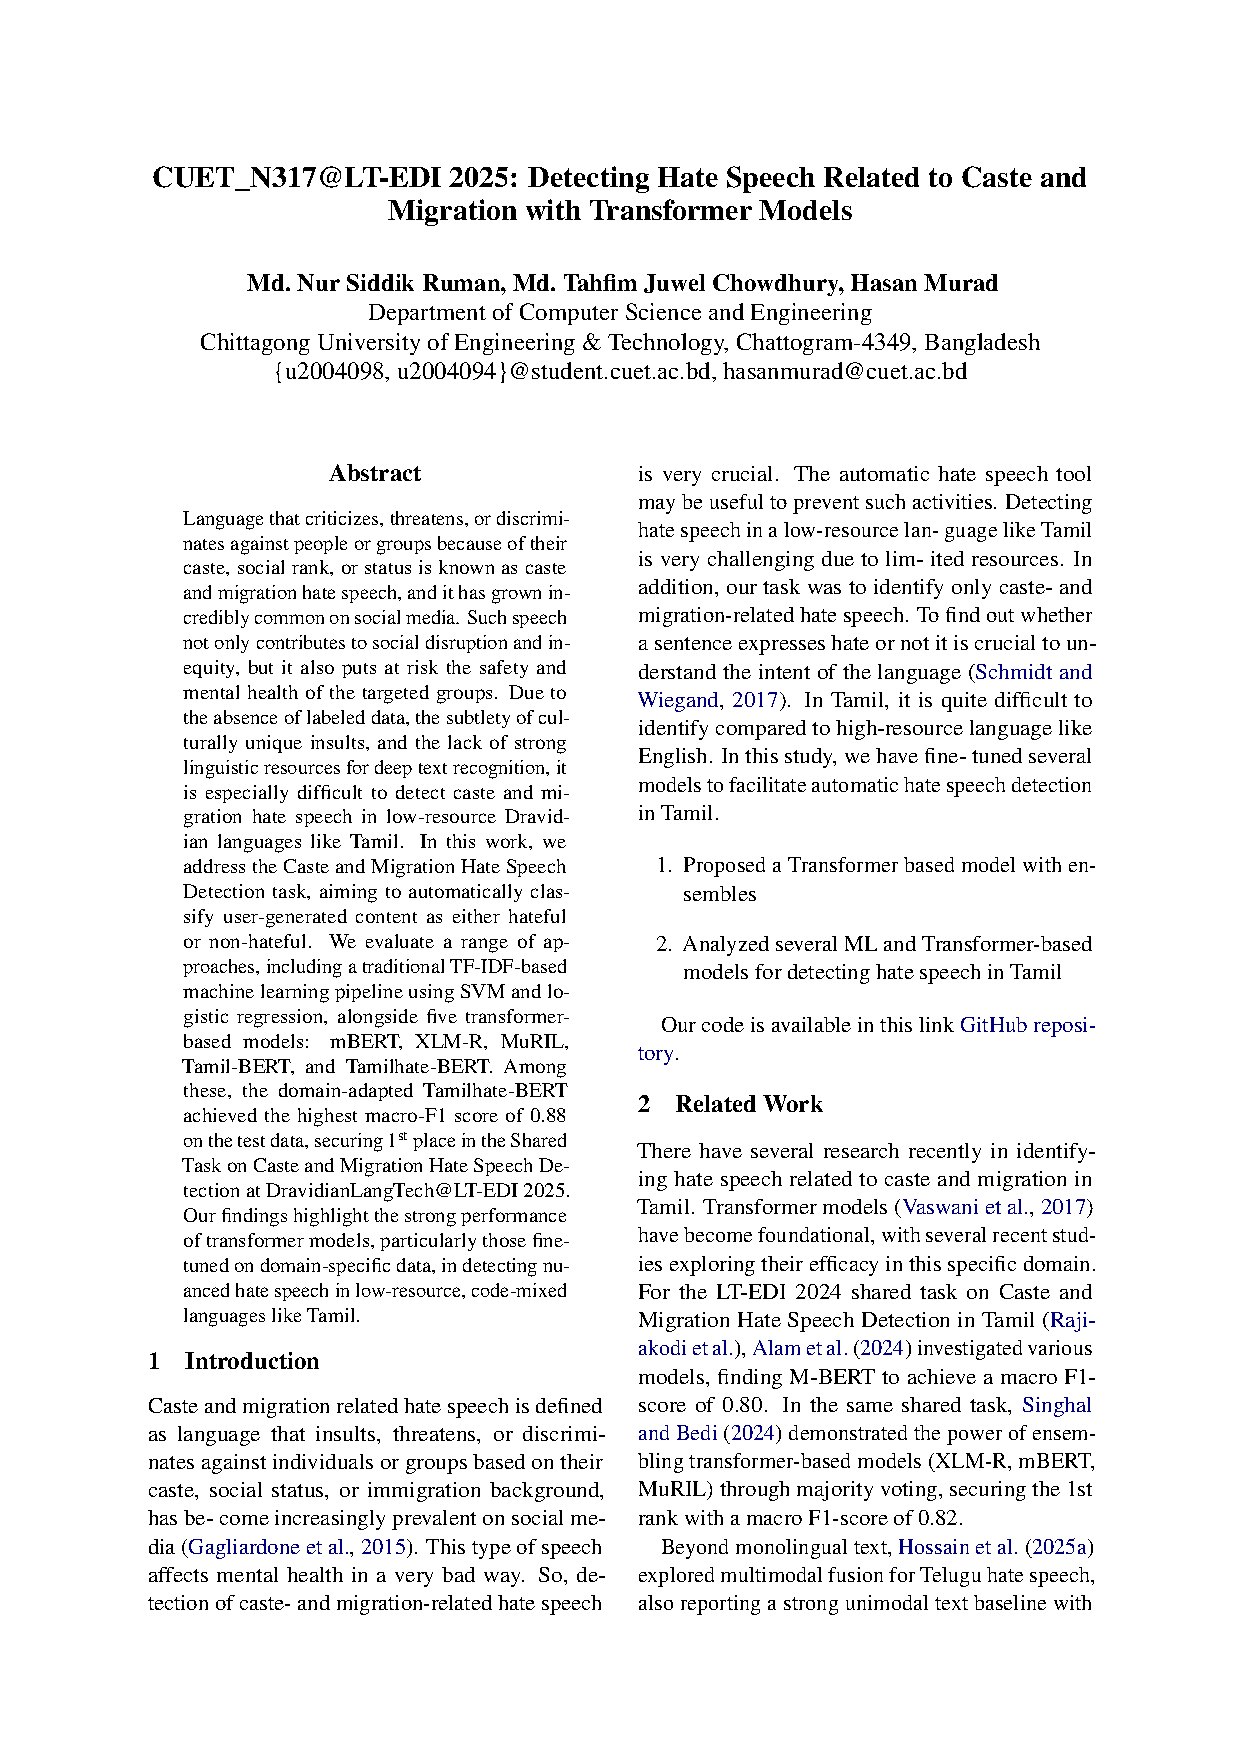
\includepdf[pagecommand={\thispagestyle{plain}},pages=-,addtotoc={1,section,1,{CUET\_N317@LT-EDI2025: Detecting Hate Speech Related to Caste and Migration with Transformer Models},ref:paper_{21}}]{LT-EDI-2025/papers/21.pdf}
  \AddToShipoutPicture*{
    \setlength{\unitlength}{1mm}
    \footnotesize

            
    \put(0,13){\parbox[t]{\paperwidth}{\centering
    							\emph{Proceedings of the Fifth Workshop on Language Technology for Equality, Diversity, Inclusion}, pages 111--115 \\
  	  						September 9, 2025 \textcopyright
  							2025 Association for Computational Linguistics}}
  }
  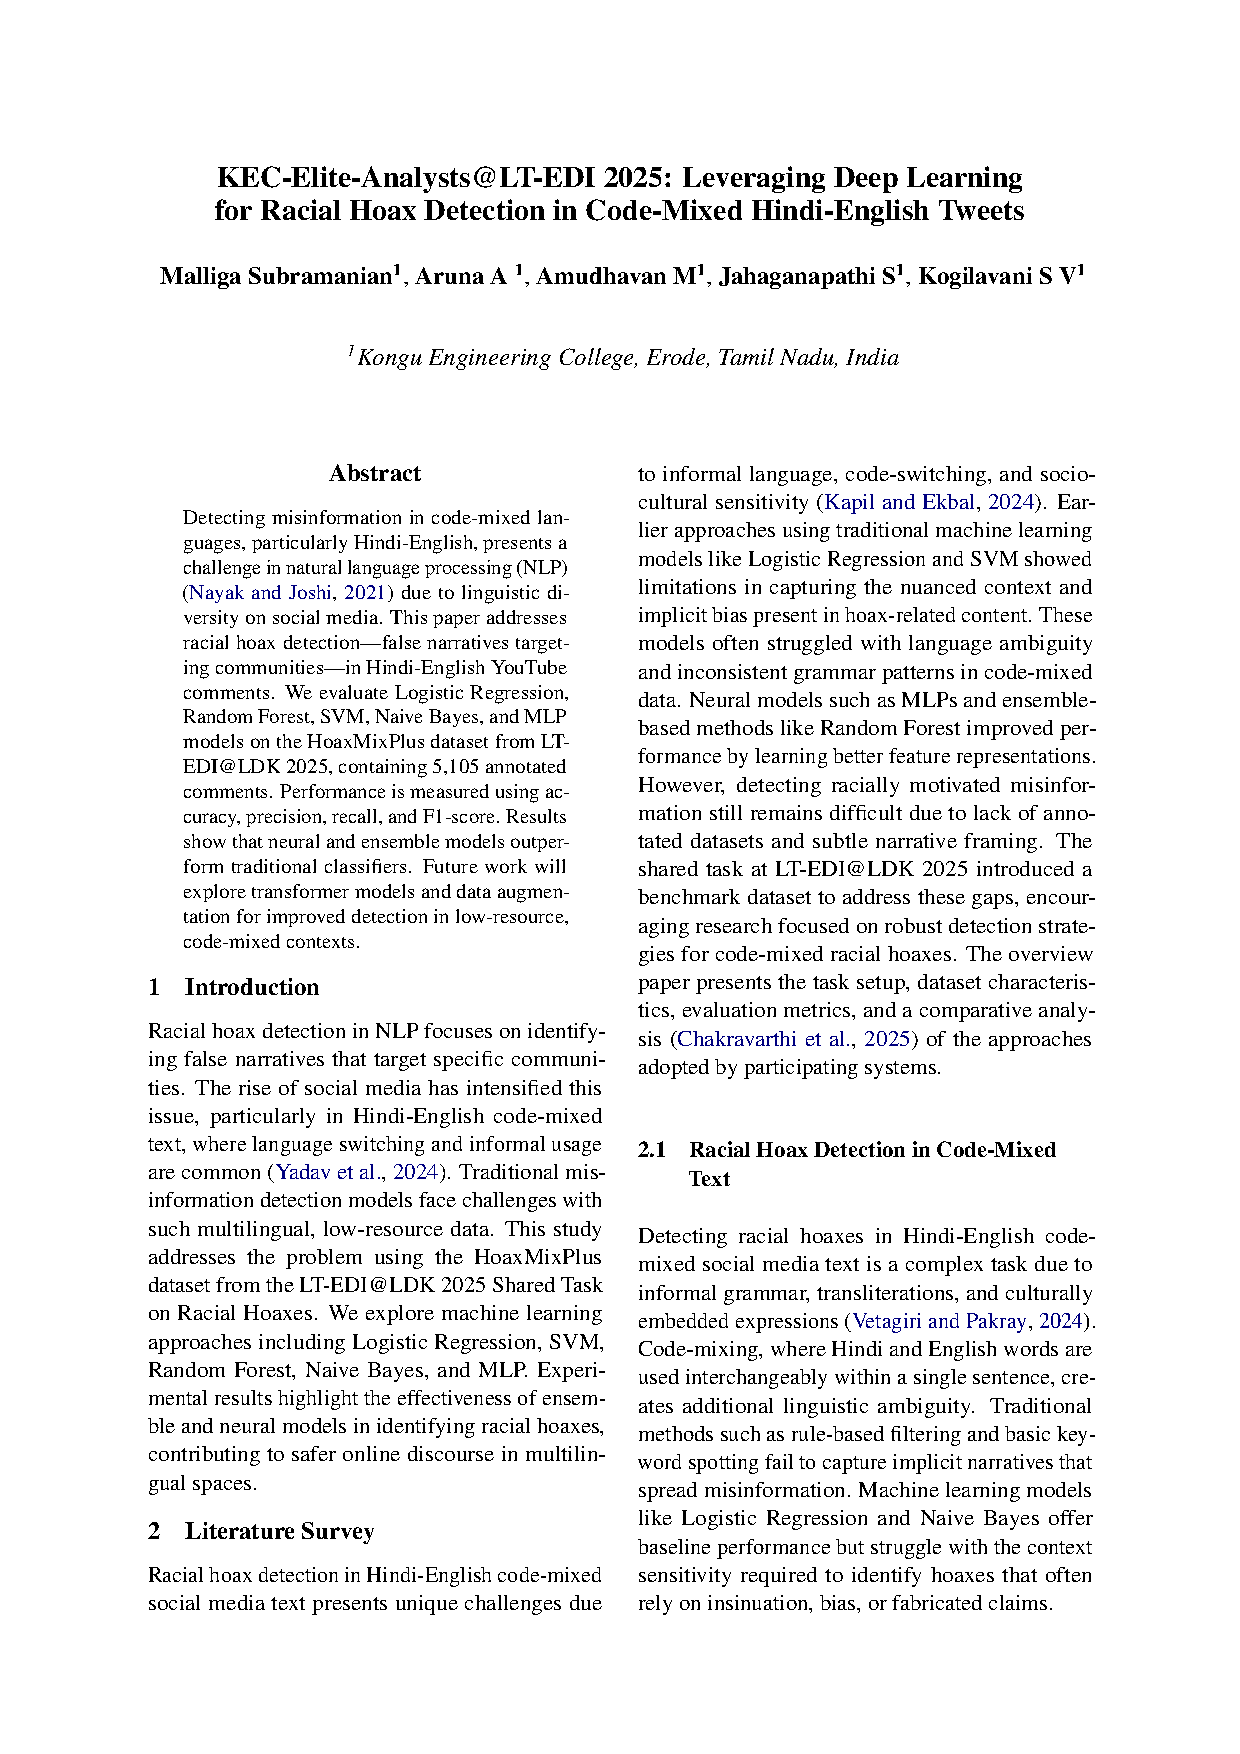
\includepdf[pagecommand={\thispagestyle{plain}},pages=-,addtotoc={1,section,1,{KEC-Elite-Analysts@LT-EDI 2025: Leveraging Deep Learning for Racial Hoax Detection in Code-Mixed Hindi-English Tweets},ref:paper_{22}}]{LT-EDI-2025/papers/22.pdf}
  \AddToShipoutPicture*{
    \setlength{\unitlength}{1mm}
    \footnotesize

            
    \put(0,13){\parbox[t]{\paperwidth}{\centering
    							\emph{Proceedings of the Fifth Workshop on Language Technology for Equality, Diversity, Inclusion}, pages 116--120 \\
  	  						September 9, 2025 \textcopyright
  							2025 Association for Computational Linguistics}}
  }
  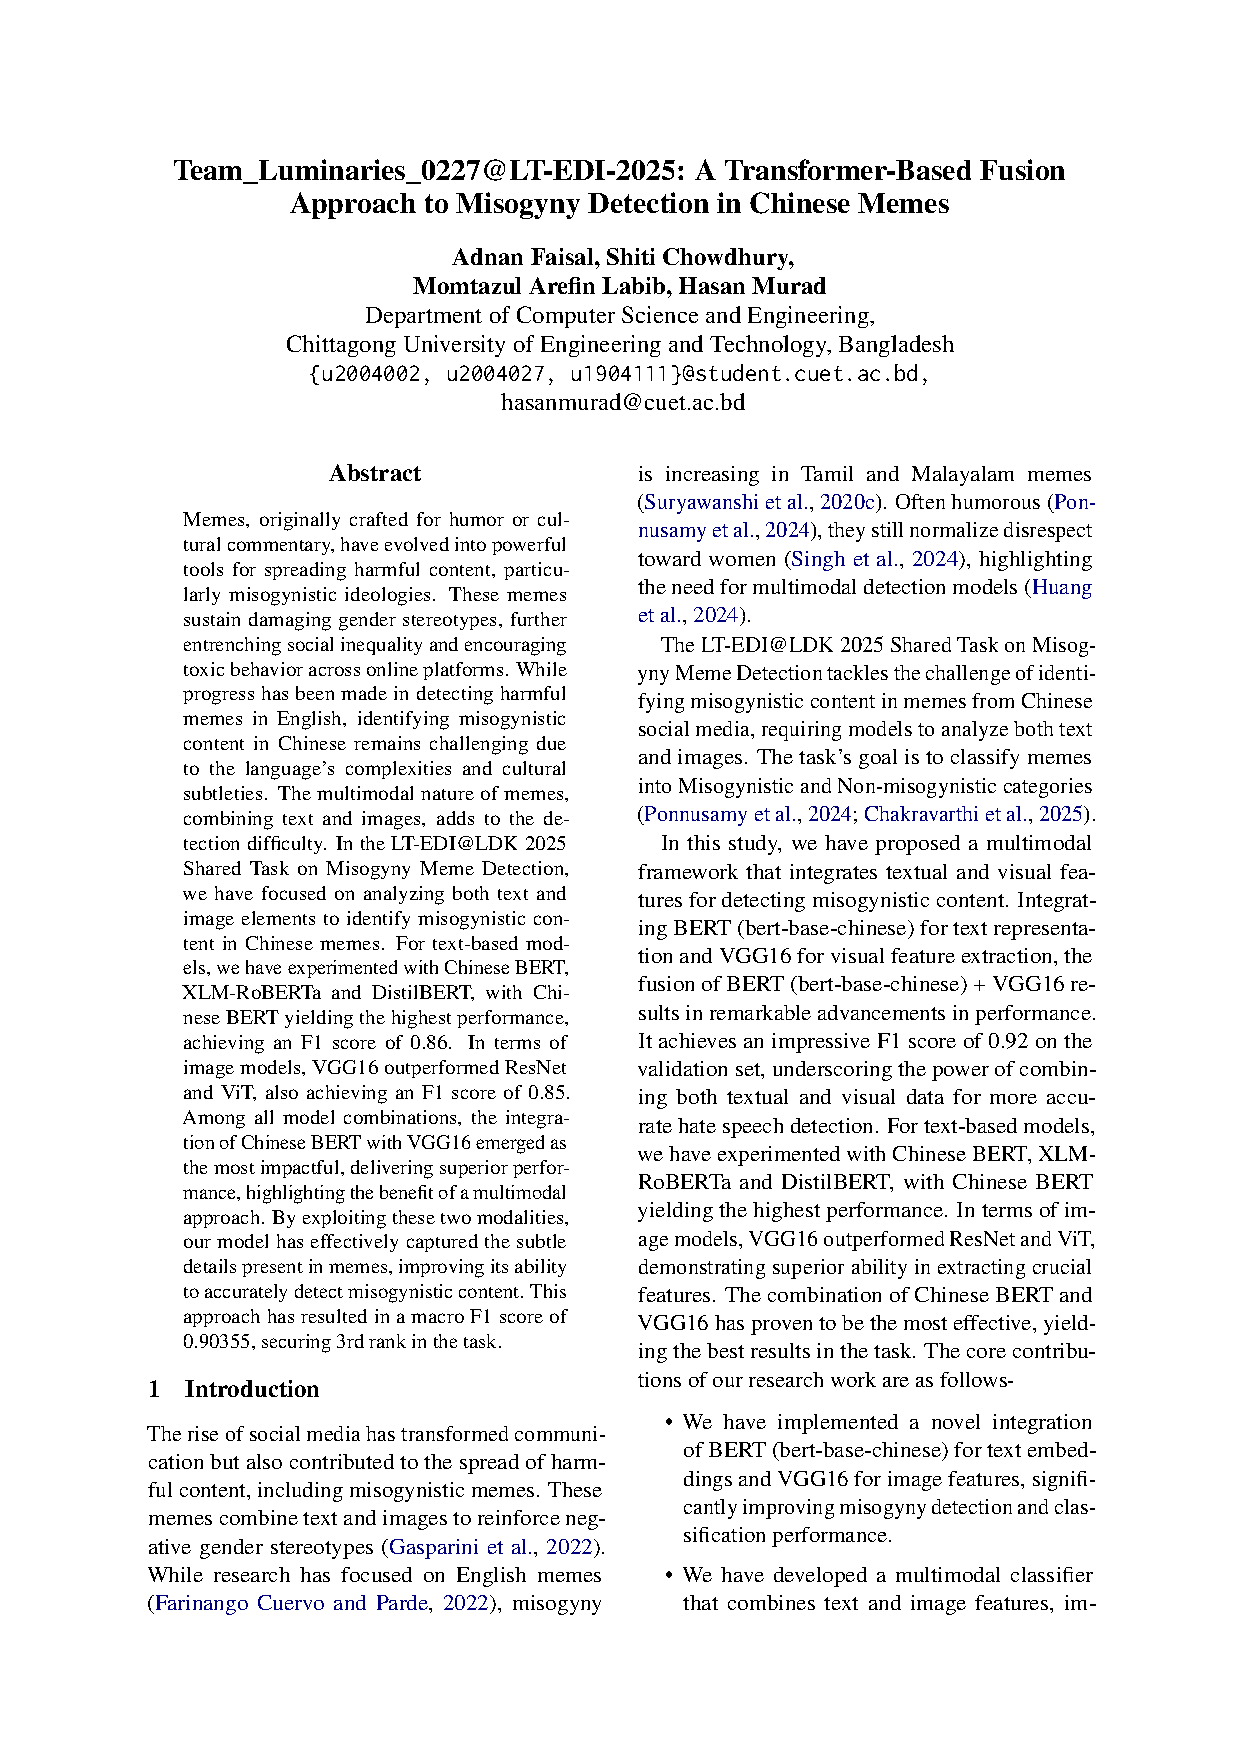
\includepdf[pagecommand={\thispagestyle{plain}},pages=-,addtotoc={1,section,1,{Team\_Luminaries\_0227@LT-EDI-2025: A Transformer-Based Fusion Approach to Misogyny Detection in Chinese Memes},ref:paper_{23}}]{LT-EDI-2025/papers/23.pdf}
  \AddToShipoutPicture*{
    \setlength{\unitlength}{1mm}
    \footnotesize

            
    \put(0,13){\parbox[t]{\paperwidth}{\centering
    							\emph{Proceedings of the Fifth Workshop on Language Technology for Equality, Diversity, Inclusion}, pages 121--126 \\
  	  						September 9, 2025 \textcopyright
  							2025 Association for Computational Linguistics}}
  }
  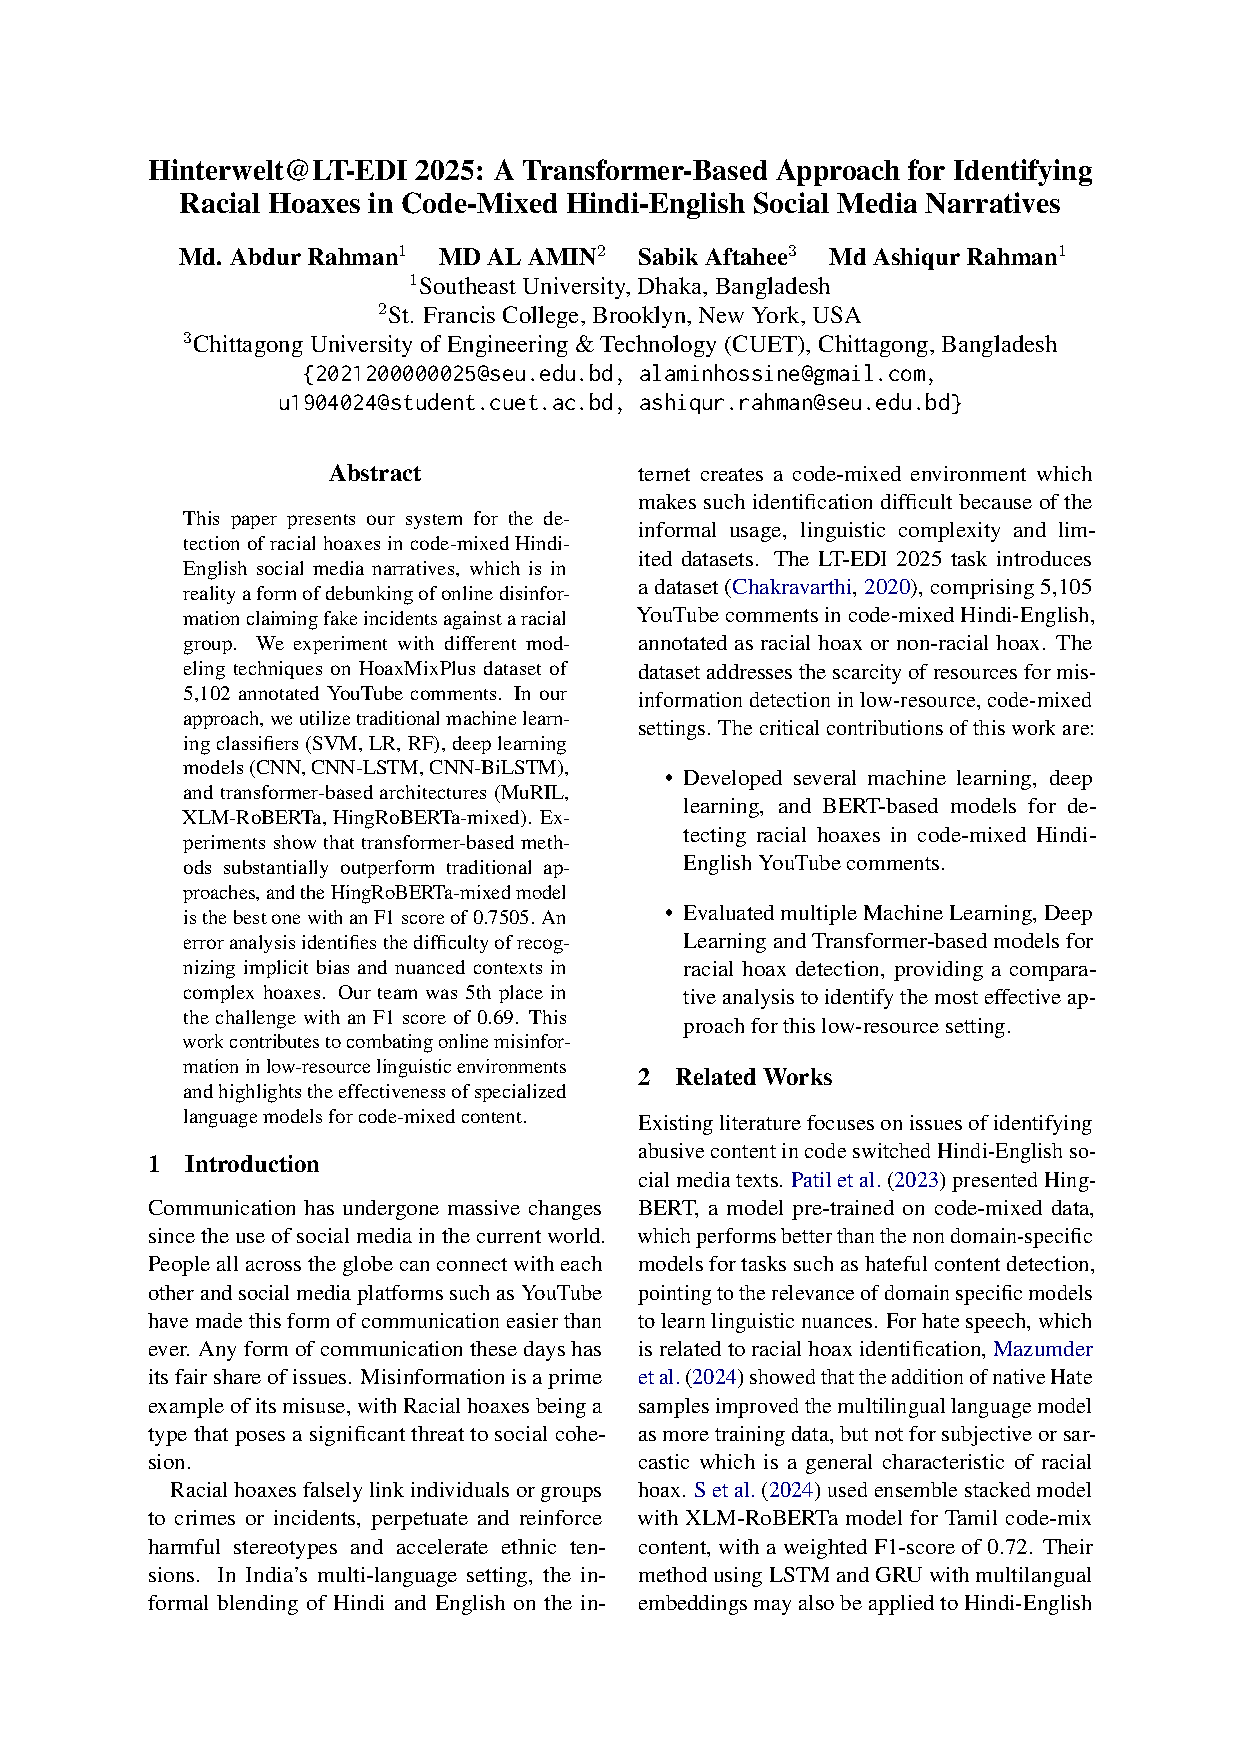
\includepdf[pagecommand={\thispagestyle{plain}},pages=-,addtotoc={1,section,1,{Hinterwelt@LT-EDI 2025: A Transformer-Based Approach for Identifying Racial Hoaxes in Code-Mixed Hindi-English Social Media Narratives},ref:paper_{24}}]{LT-EDI-2025/papers/24.pdf}
  \AddToShipoutPicture*{
    \setlength{\unitlength}{1mm}
    \footnotesize

            
    \put(0,13){\parbox[t]{\paperwidth}{\centering
    							\emph{Proceedings of the Fifth Workshop on Language Technology for Equality, Diversity, Inclusion}, pages 127--132 \\
  	  						September 9, 2025 \textcopyright
  							2025 Association for Computational Linguistics}}
  }
  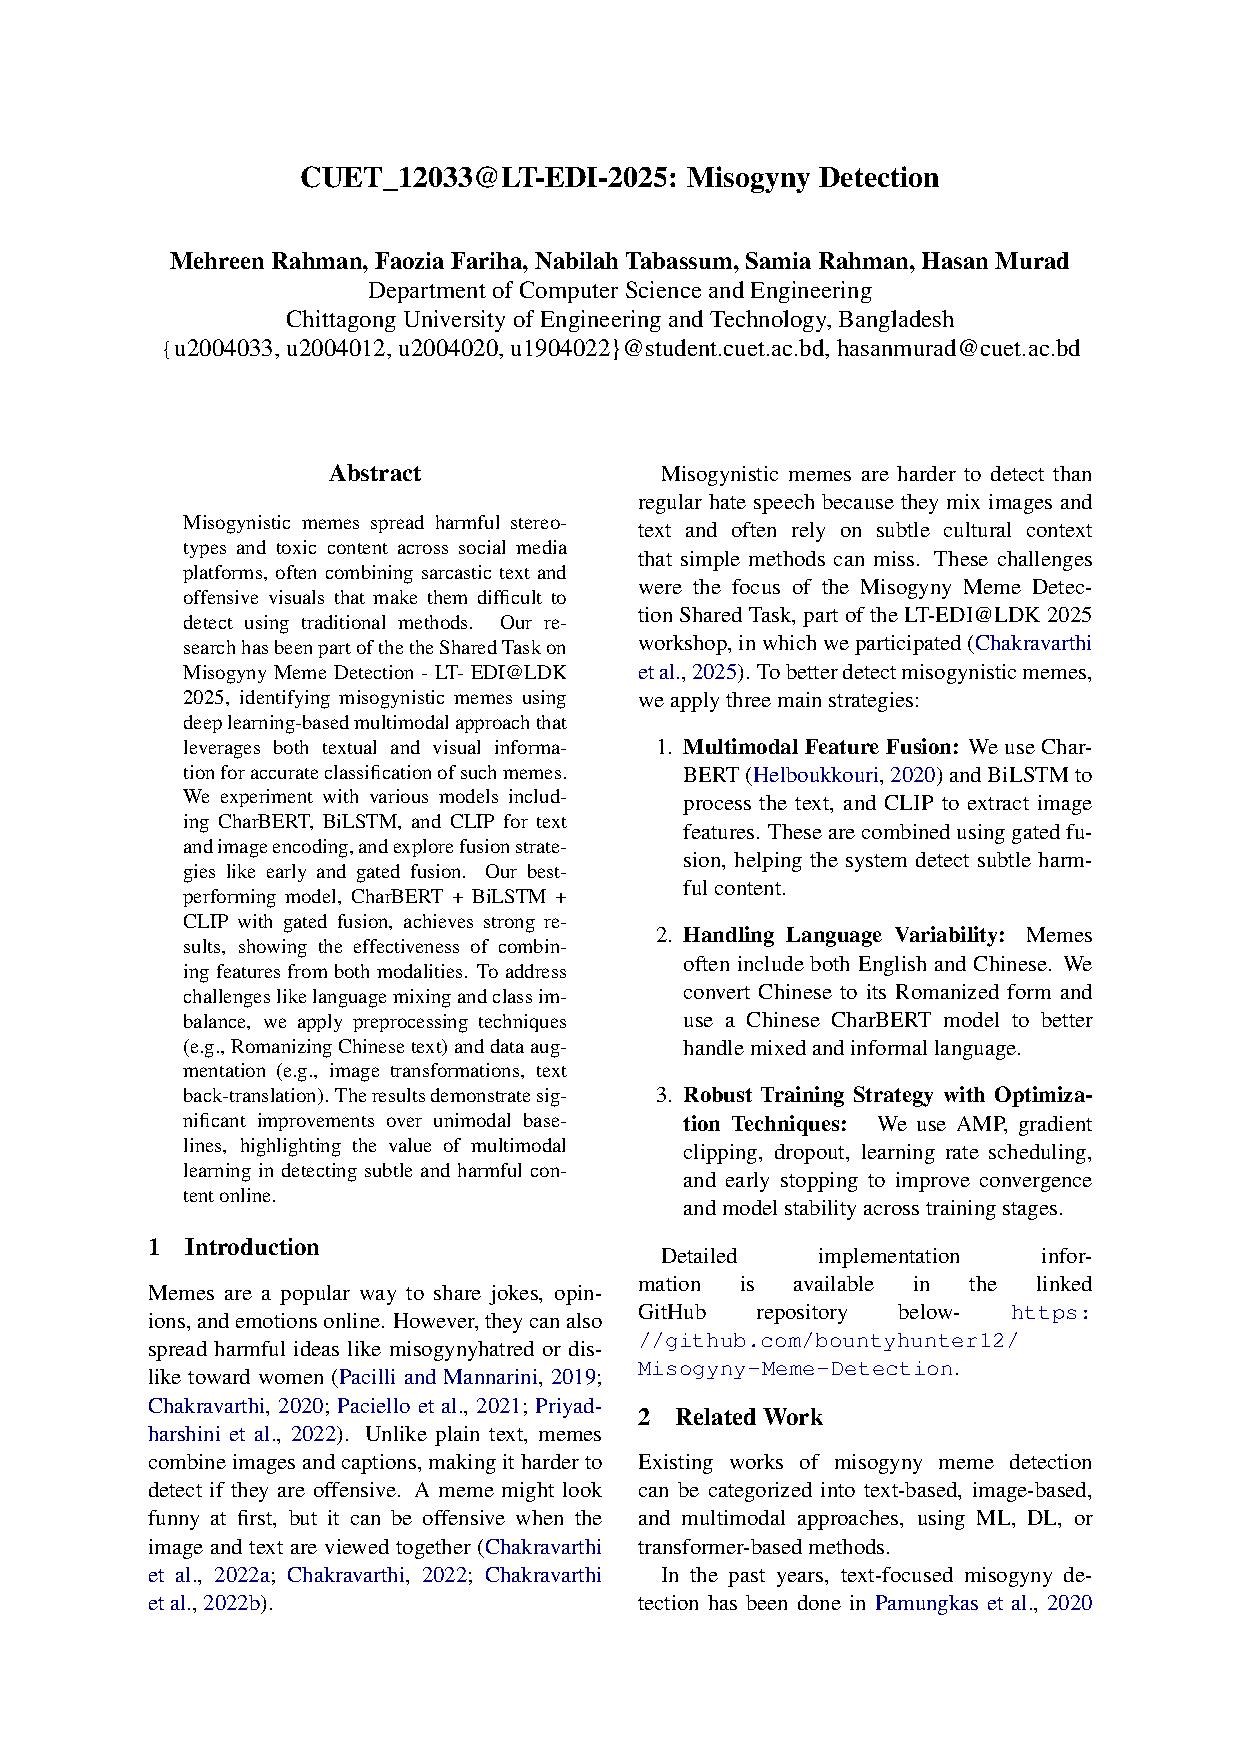
\includepdf[pagecommand={\thispagestyle{plain}},pages=-,addtotoc={1,section,1,{CUET\_12033@LT-EDI-2025: Misogyny Detection},ref:paper_{25}}]{LT-EDI-2025/papers/25.pdf}
  \AddToShipoutPicture*{
    \setlength{\unitlength}{1mm}
    \footnotesize

            
    \put(0,13){\parbox[t]{\paperwidth}{\centering
    							\emph{Proceedings of the Fifth Workshop on Language Technology for Equality, Diversity, Inclusion}, pages 133--139 \\
  	  						September 9, 2025 \textcopyright
  							2025 Association for Computational Linguistics}}
  }
  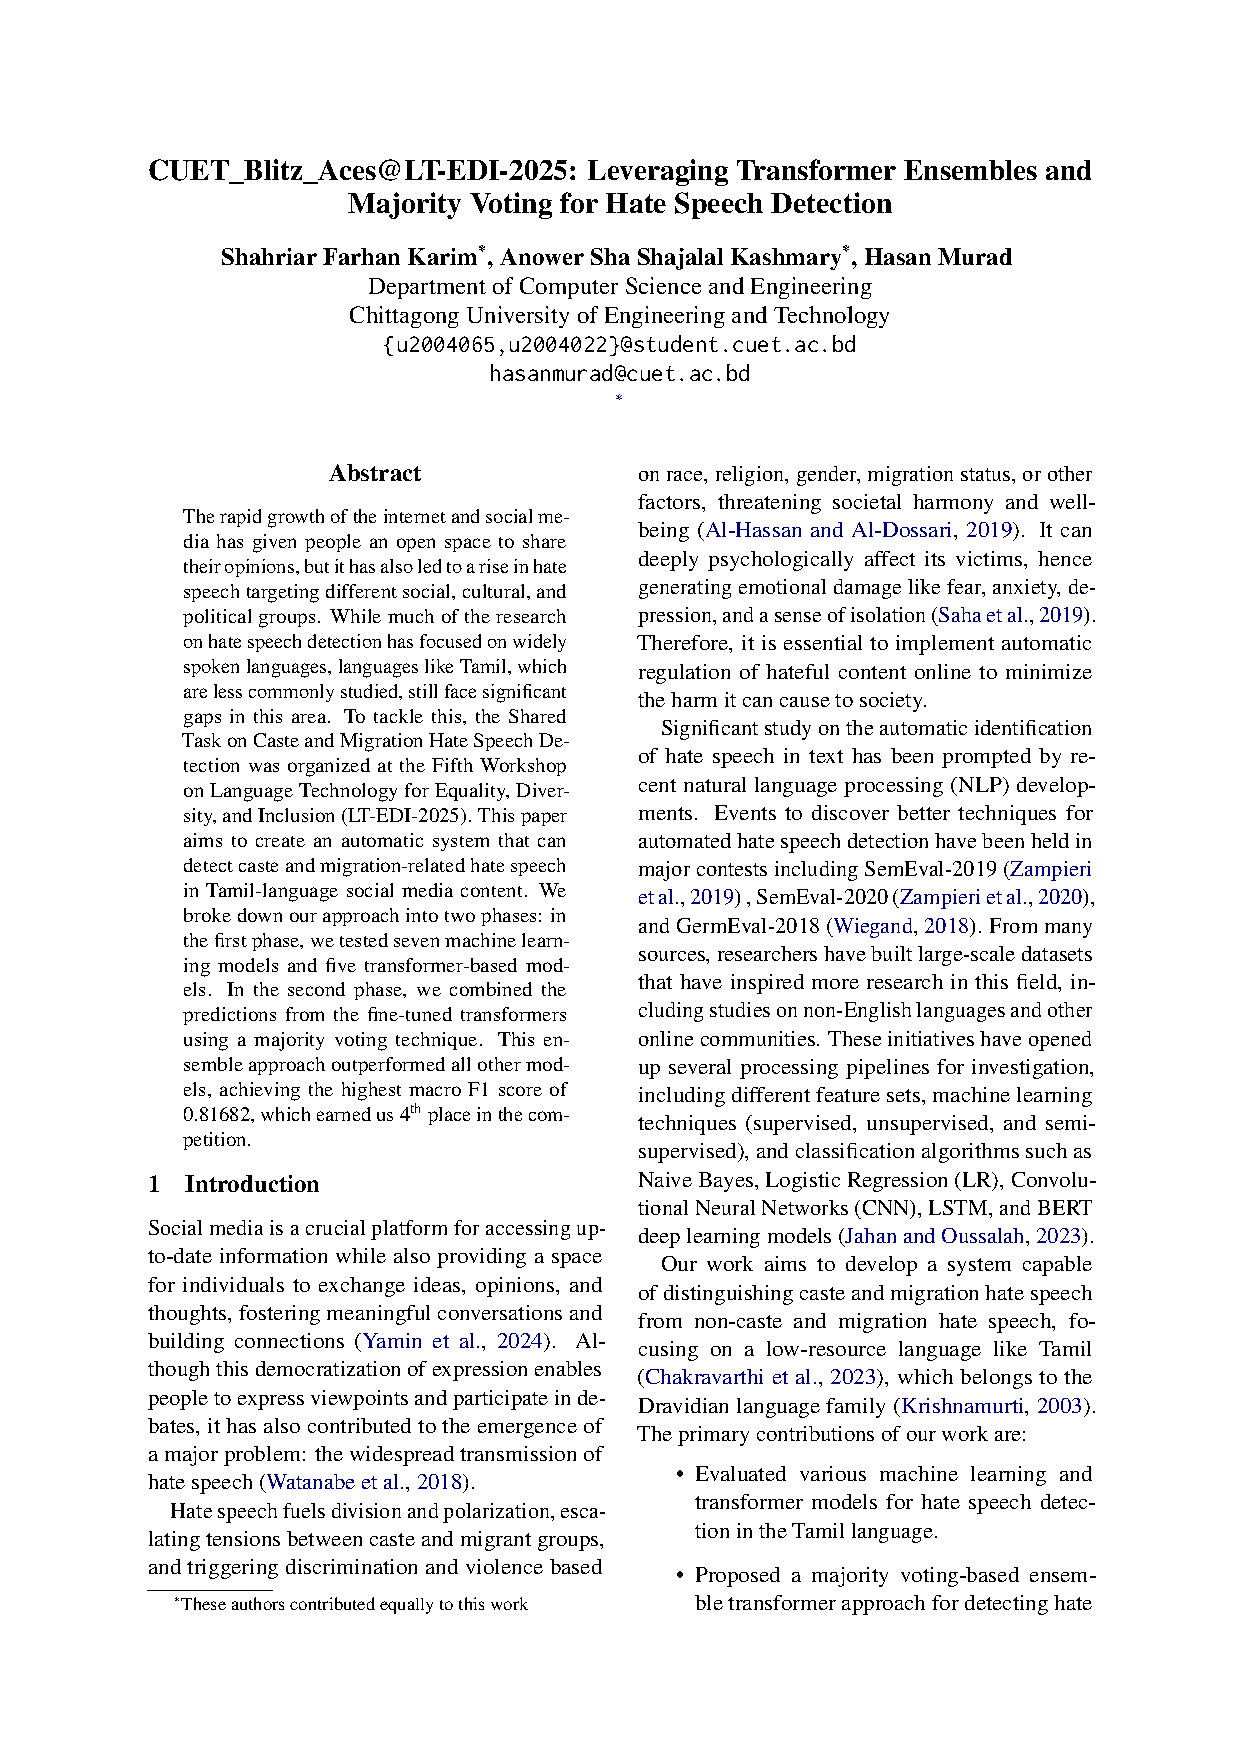
\includepdf[pagecommand={\thispagestyle{plain}},pages=-,addtotoc={1,section,1,{CUET\_Blitz\_Aces@LT-EDI-2025: Leveraging Transformer Ensembles and Majority Voting for Hate Speech Detection},ref:paper_{26}}]{LT-EDI-2025/papers/26.pdf}
  \AddToShipoutPicture*{
    \setlength{\unitlength}{1mm}
    \footnotesize

            
    \put(0,13){\parbox[t]{\paperwidth}{\centering
    							\emph{Proceedings of the Fifth Workshop on Language Technology for Equality, Diversity, Inclusion}, pages 140--145 \\
  	  						September 9, 2025 \textcopyright
  							2025 Association for Computational Linguistics}}
  }
  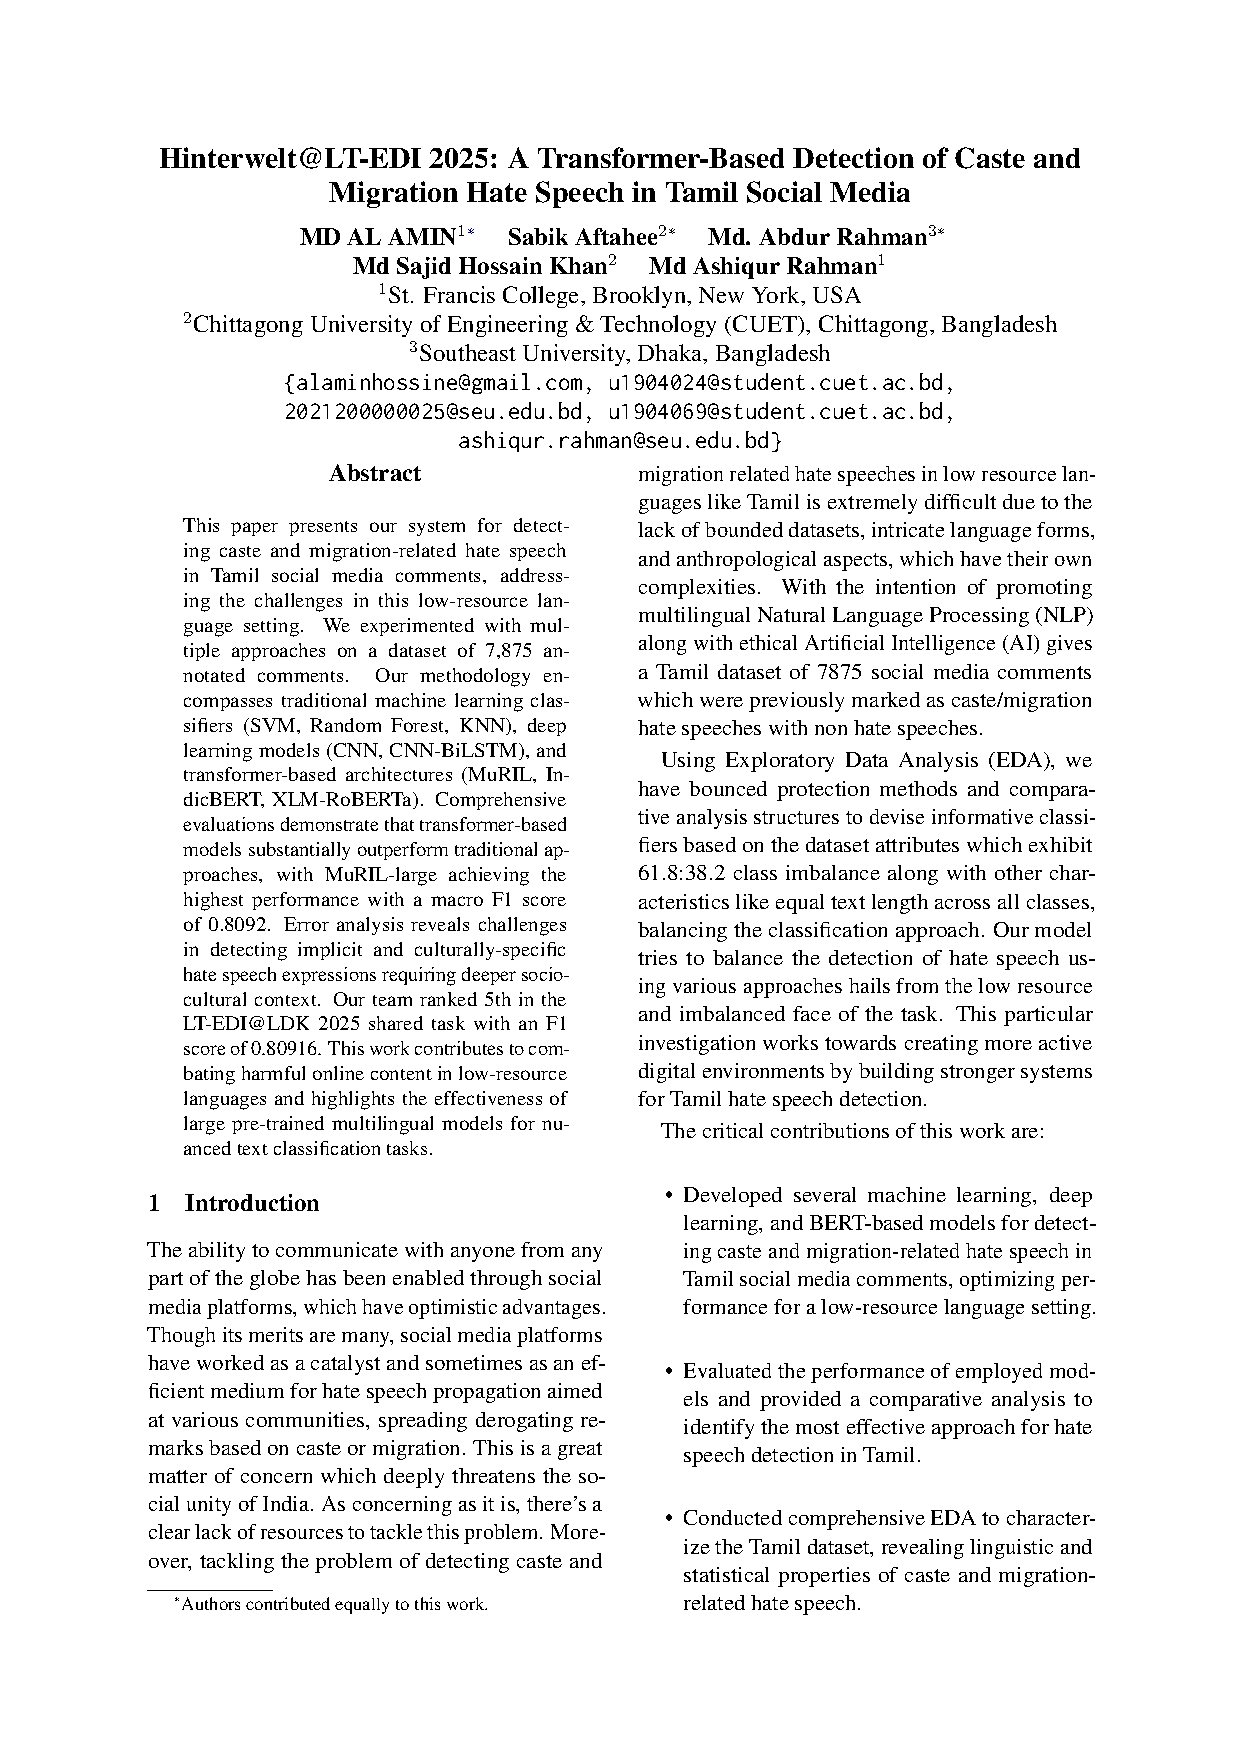
\includepdf[pagecommand={\thispagestyle{plain}},pages=-,addtotoc={1,section,1,{Hinterwelt@LT-EDI 2025: A Transformer-Based Detection of Caste and Migration Hate Speech in Tamil Social Media},ref:paper_{27}}]{LT-EDI-2025/papers/27.pdf}
  \AddToShipoutPicture*{
    \setlength{\unitlength}{1mm}
    \footnotesize

            
    \put(0,13){\parbox[t]{\paperwidth}{\centering
    							\emph{Proceedings of the Fifth Workshop on Language Technology for Equality, Diversity, Inclusion}, pages 146--151 \\
  	  						September 9, 2025 \textcopyright
  							2025 Association for Computational Linguistics}}
  }
  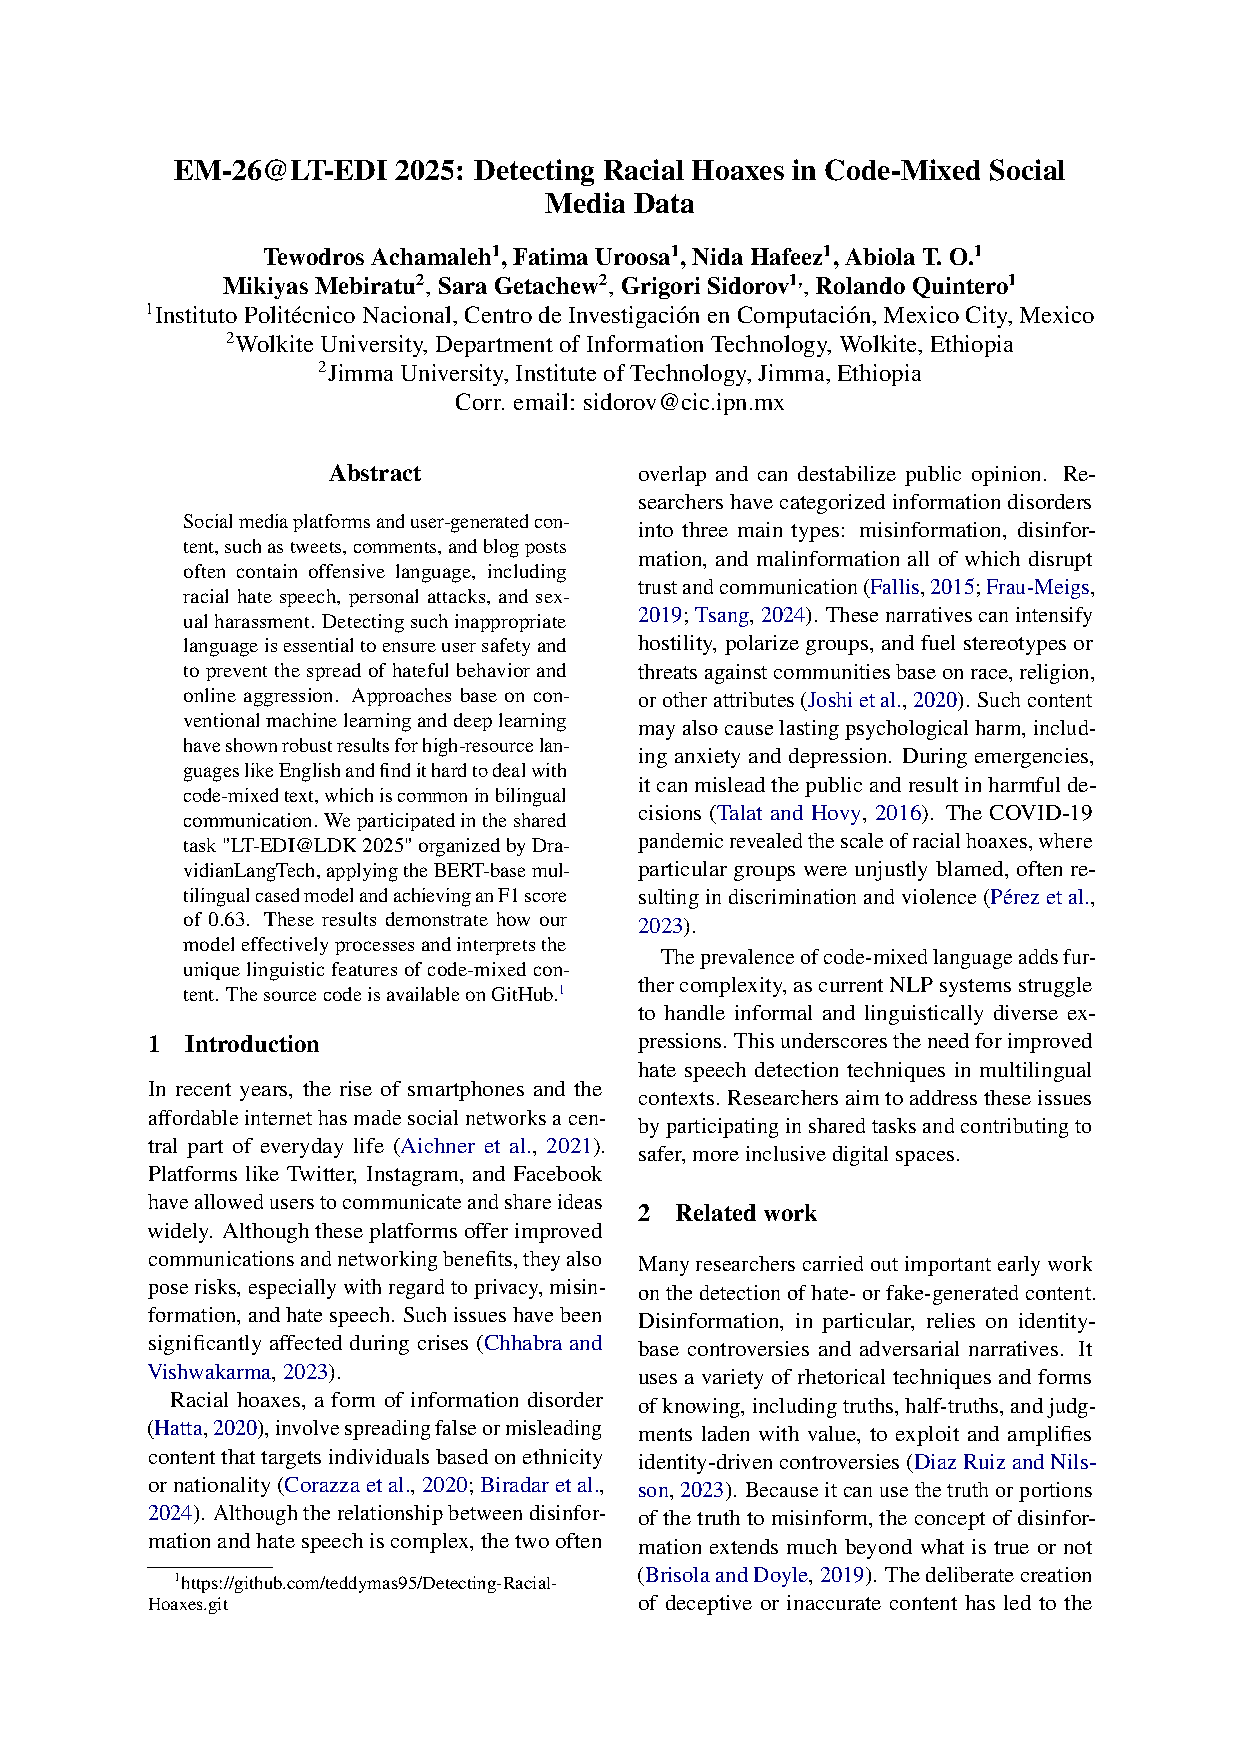
\includepdf[pagecommand={\thispagestyle{plain}},pages=-,addtotoc={1,section,1,{EM-26@LT-EDI 2025: Detecting Racial Hoaxes in Code-Mixed Social Media Data},ref:paper_{28}}]{LT-EDI-2025/papers/28.pdf}
  \AddToShipoutPicture*{
    \setlength{\unitlength}{1mm}
    \footnotesize

            
    \put(0,13){\parbox[t]{\paperwidth}{\centering
    							\emph{Proceedings of the Fifth Workshop on Language Technology for Equality, Diversity, Inclusion}, pages 152--158 \\
  	  						September 9, 2025 \textcopyright
  							2025 Association for Computational Linguistics}}
  }
  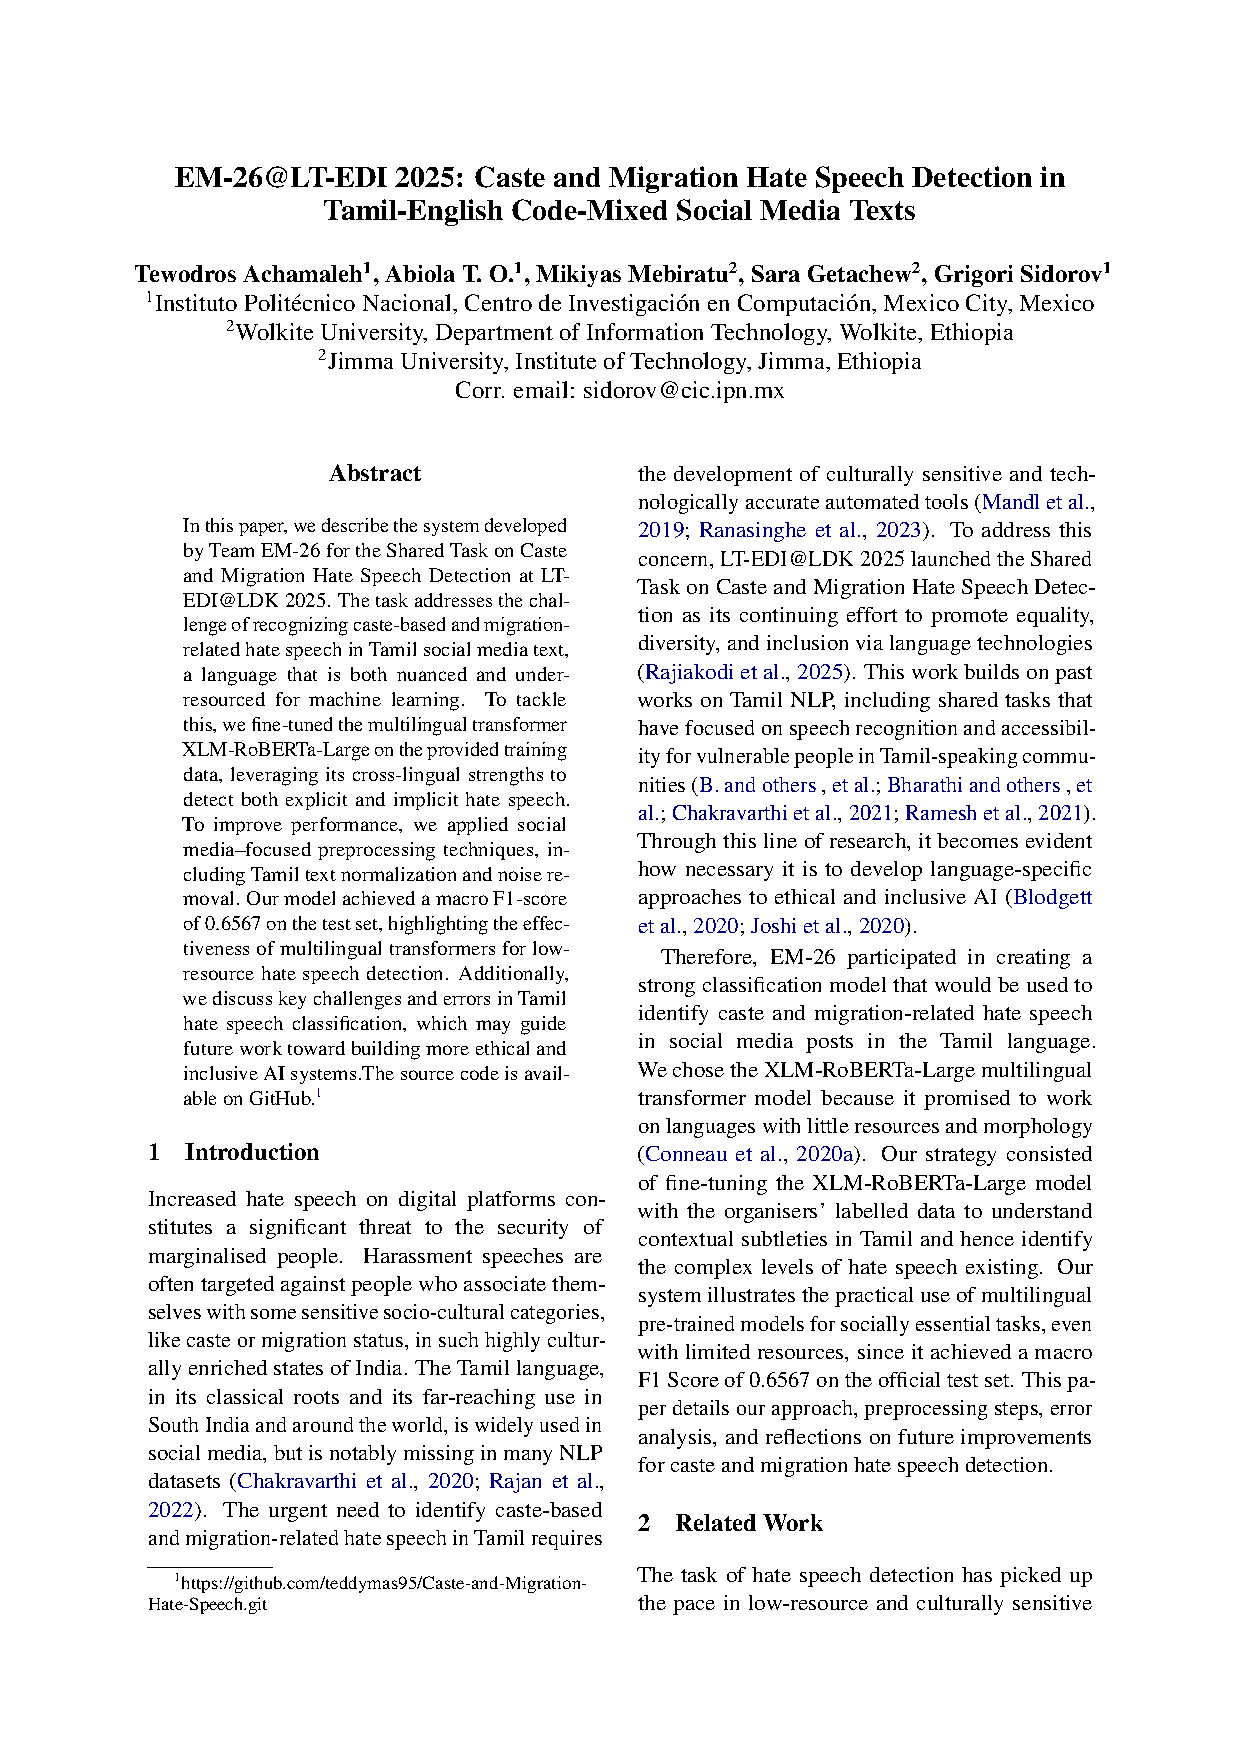
\includepdf[pagecommand={\thispagestyle{plain}},pages=-,addtotoc={1,section,1,{EM-26@LT-EDI 2025: Caste and Migration Hate Speech Detection in Tamil-English Code-Mixed Social Media Texts},ref:paper_{29}}]{LT-EDI-2025/papers/29.pdf}
  \AddToShipoutPicture*{
    \setlength{\unitlength}{1mm}
    \footnotesize

            
    \put(0,13){\parbox[t]{\paperwidth}{\centering
    							\emph{Proceedings of the Fifth Workshop on Language Technology for Equality, Diversity, Inclusion}, pages 159--170 \\
  	  						September 9, 2025 \textcopyright
  							2025 Association for Computational Linguistics}}
  }
  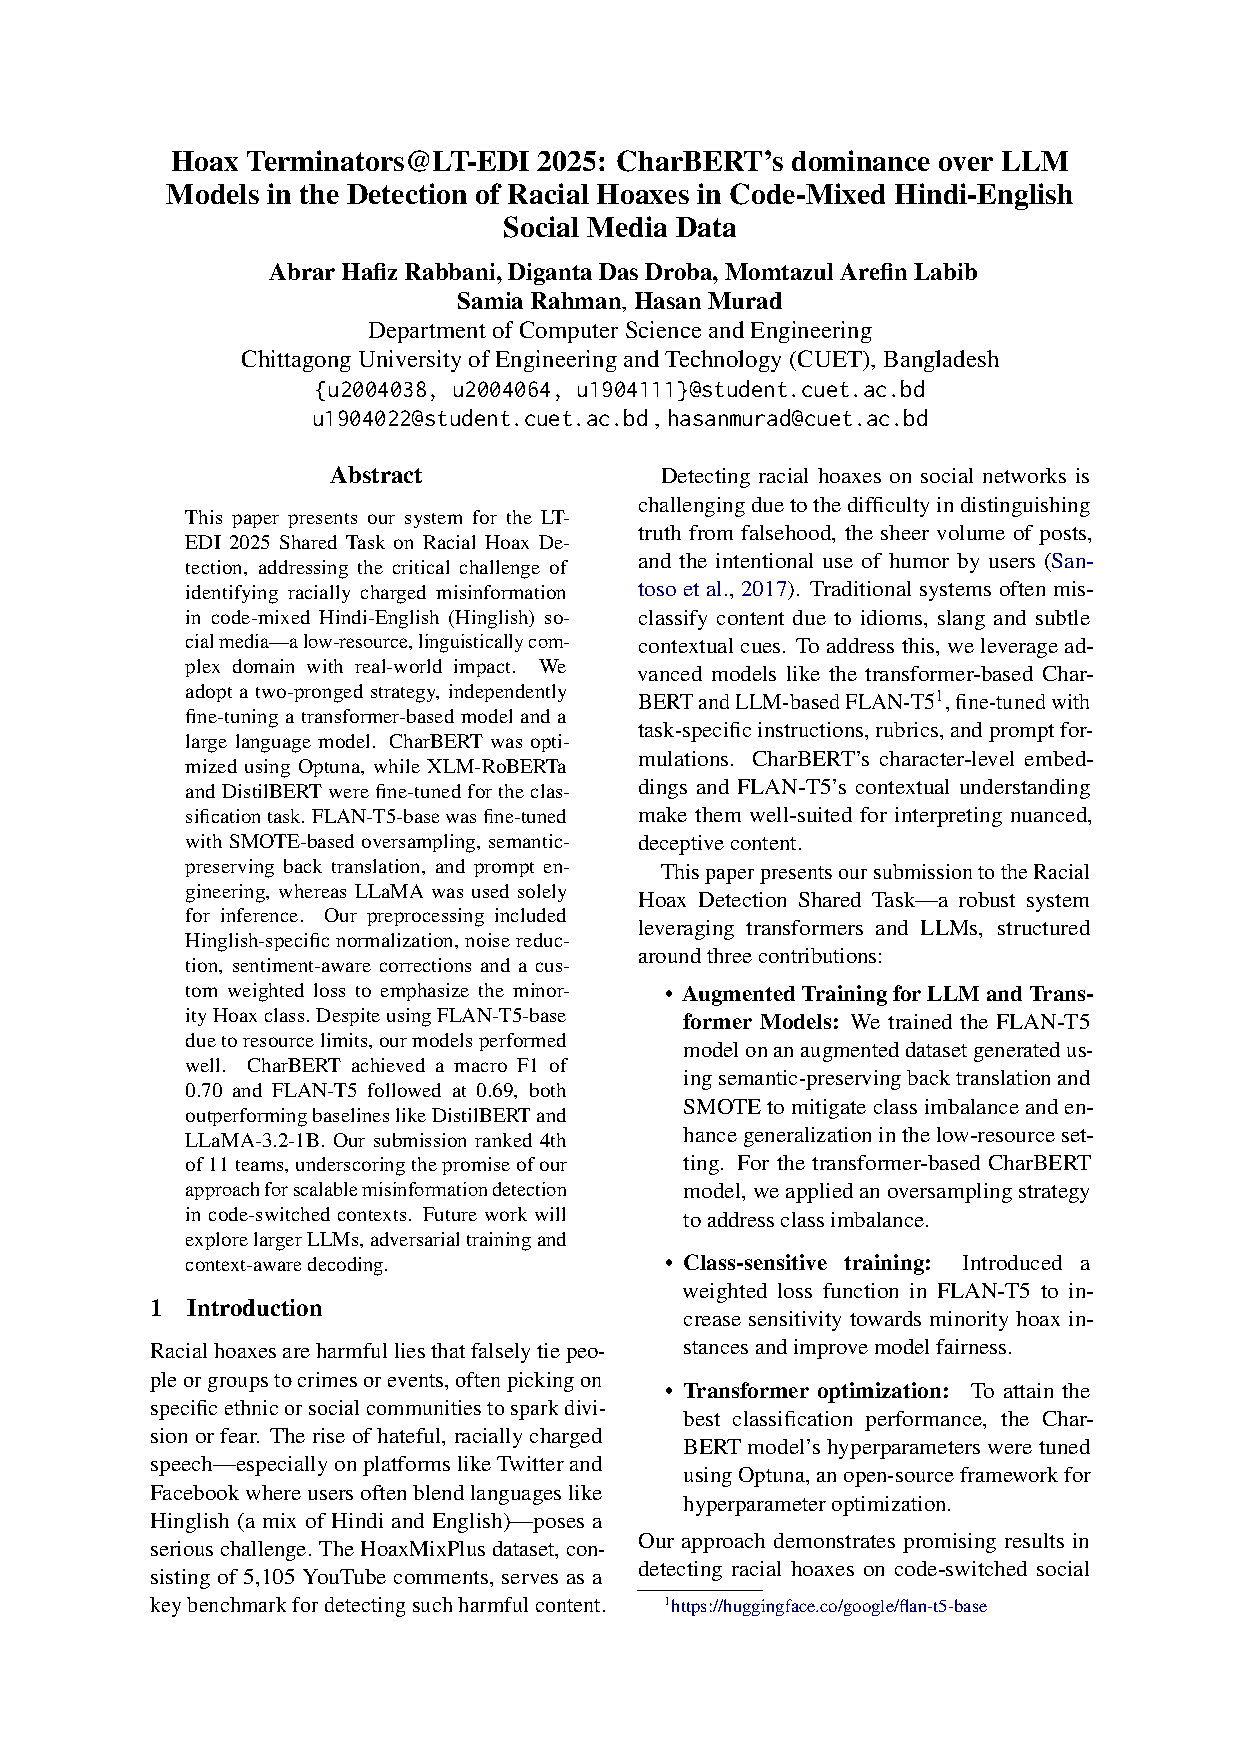
\includepdf[pagecommand={\thispagestyle{plain}},pages=-,addtotoc={1,section,1,{Hoax Terminators@LT-EDI 2025: CharBERT's dominance over LLM Models in the Detection of Racial Hoaxes in Code-Mixed Hindi-English Social Media Data},ref:paper_{30}}]{LT-EDI-2025/papers/30.pdf}
  \AddToShipoutPicture*{
    \setlength{\unitlength}{1mm}
    \footnotesize

            
    \put(0,13){\parbox[t]{\paperwidth}{\centering
    							\emph{Proceedings of the Fifth Workshop on Language Technology for Equality, Diversity, Inclusion}, pages 171--176 \\
  	  						September 9, 2025 \textcopyright
  							2025 Association for Computational Linguistics}}
  }
  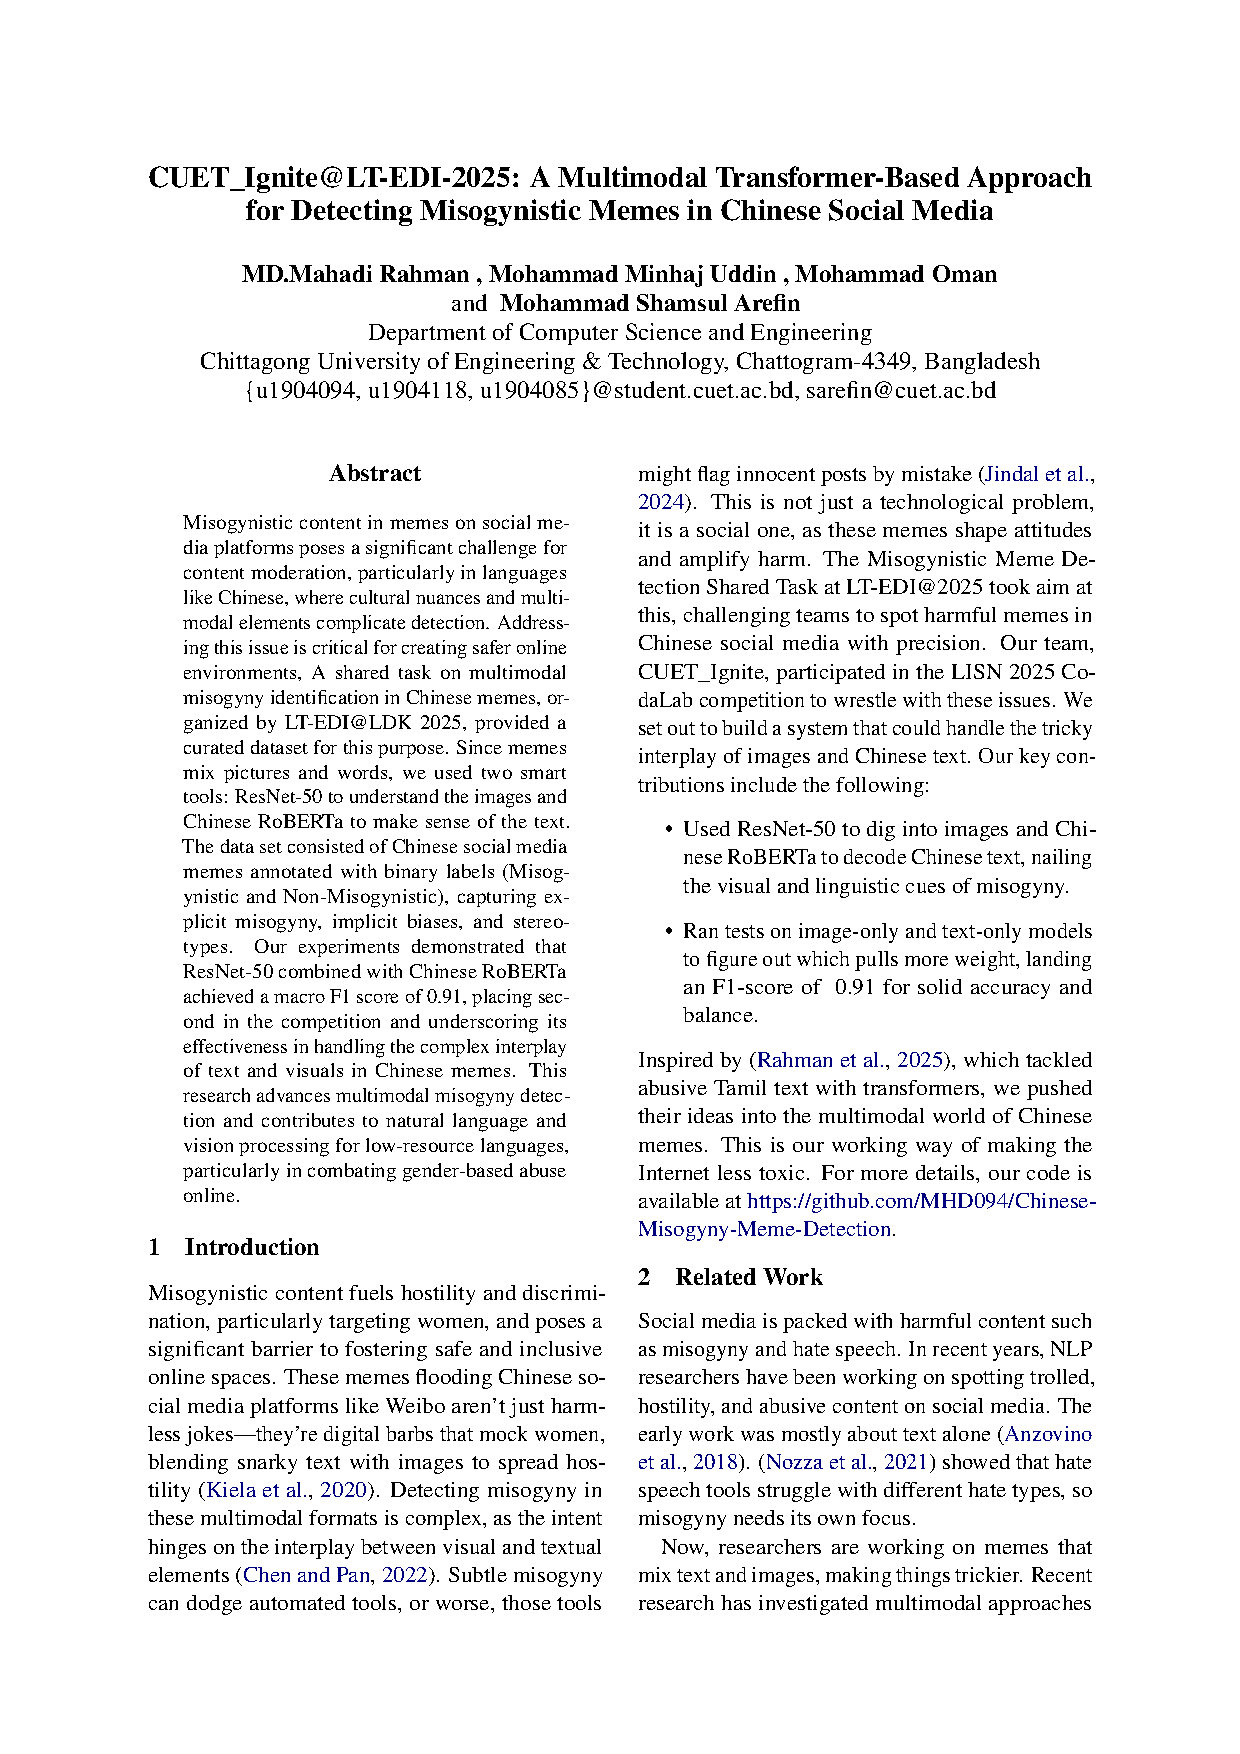
\includepdf[pagecommand={\thispagestyle{plain}},pages=-,addtotoc={1,section,1,{CUET\_Ignite@LT-EDI-2025: A Multimodal Transformer-Based Approach for Detecting Misogynistic Memes in Chinese Social Media},ref:paper_{31}}]{LT-EDI-2025/papers/31.pdf}
  \AddToShipoutPicture*{
    \setlength{\unitlength}{1mm}
    \footnotesize

            
    \put(0,13){\parbox[t]{\paperwidth}{\centering
    							\emph{Proceedings of the Fifth Workshop on Language Technology for Equality, Diversity, Inclusion}, pages 177--182 \\
  	  						September 9, 2025 \textcopyright
  							2025 Association for Computational Linguistics}}
  }
  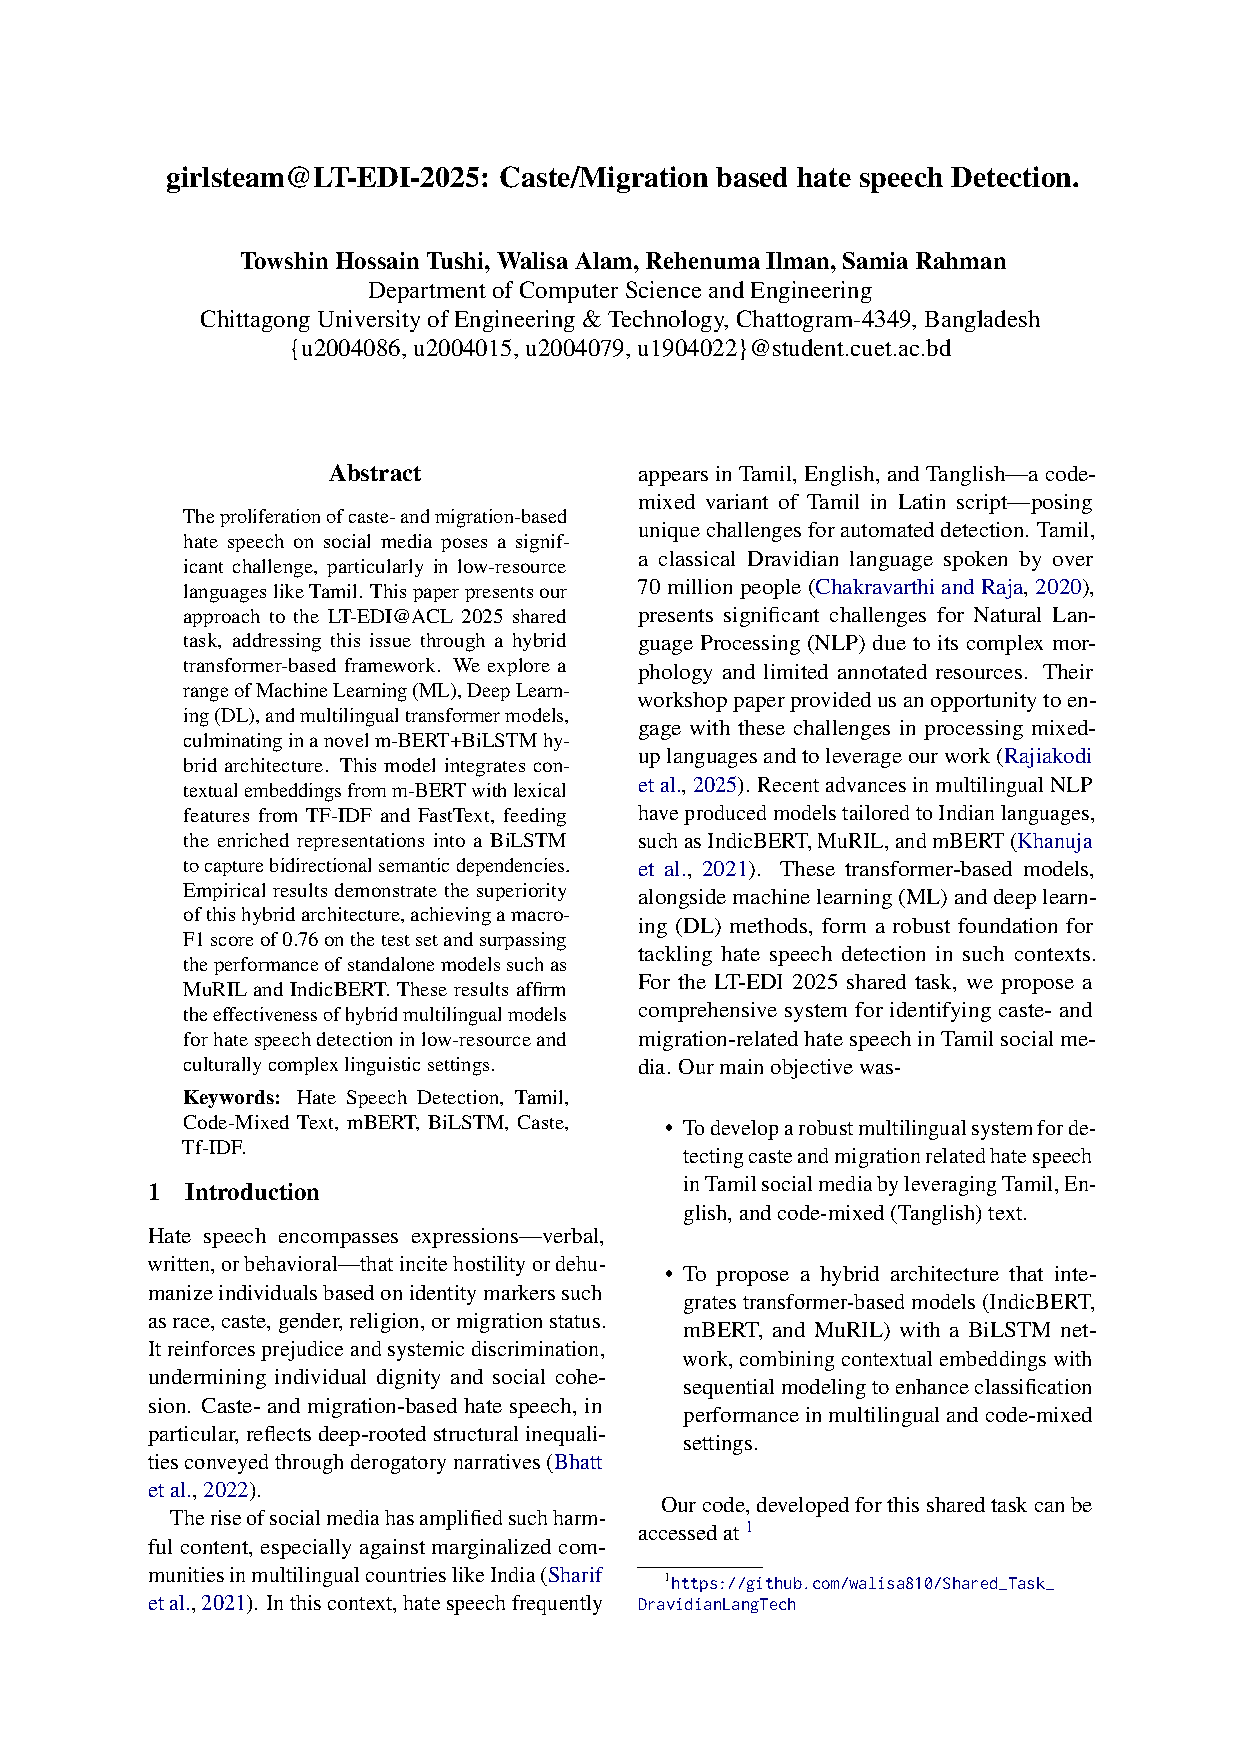
\includepdf[pagecommand={\thispagestyle{plain}},pages=-,addtotoc={1,section,1,{girlsteam@LT-EDI-2025: Caste/Migration based hate speech Detection},ref:paper_{32}}]{LT-EDI-2025/papers/32.pdf}
  \AddToShipoutPicture*{
    \setlength{\unitlength}{1mm}
    \footnotesize

            
    \put(0,13){\parbox[t]{\paperwidth}{\centering
    							\emph{Proceedings of the Fifth Workshop on Language Technology for Equality, Diversity, Inclusion}, pages 183--188 \\
  	  						September 9, 2025 \textcopyright
  							2025 Association for Computational Linguistics}}
  }
  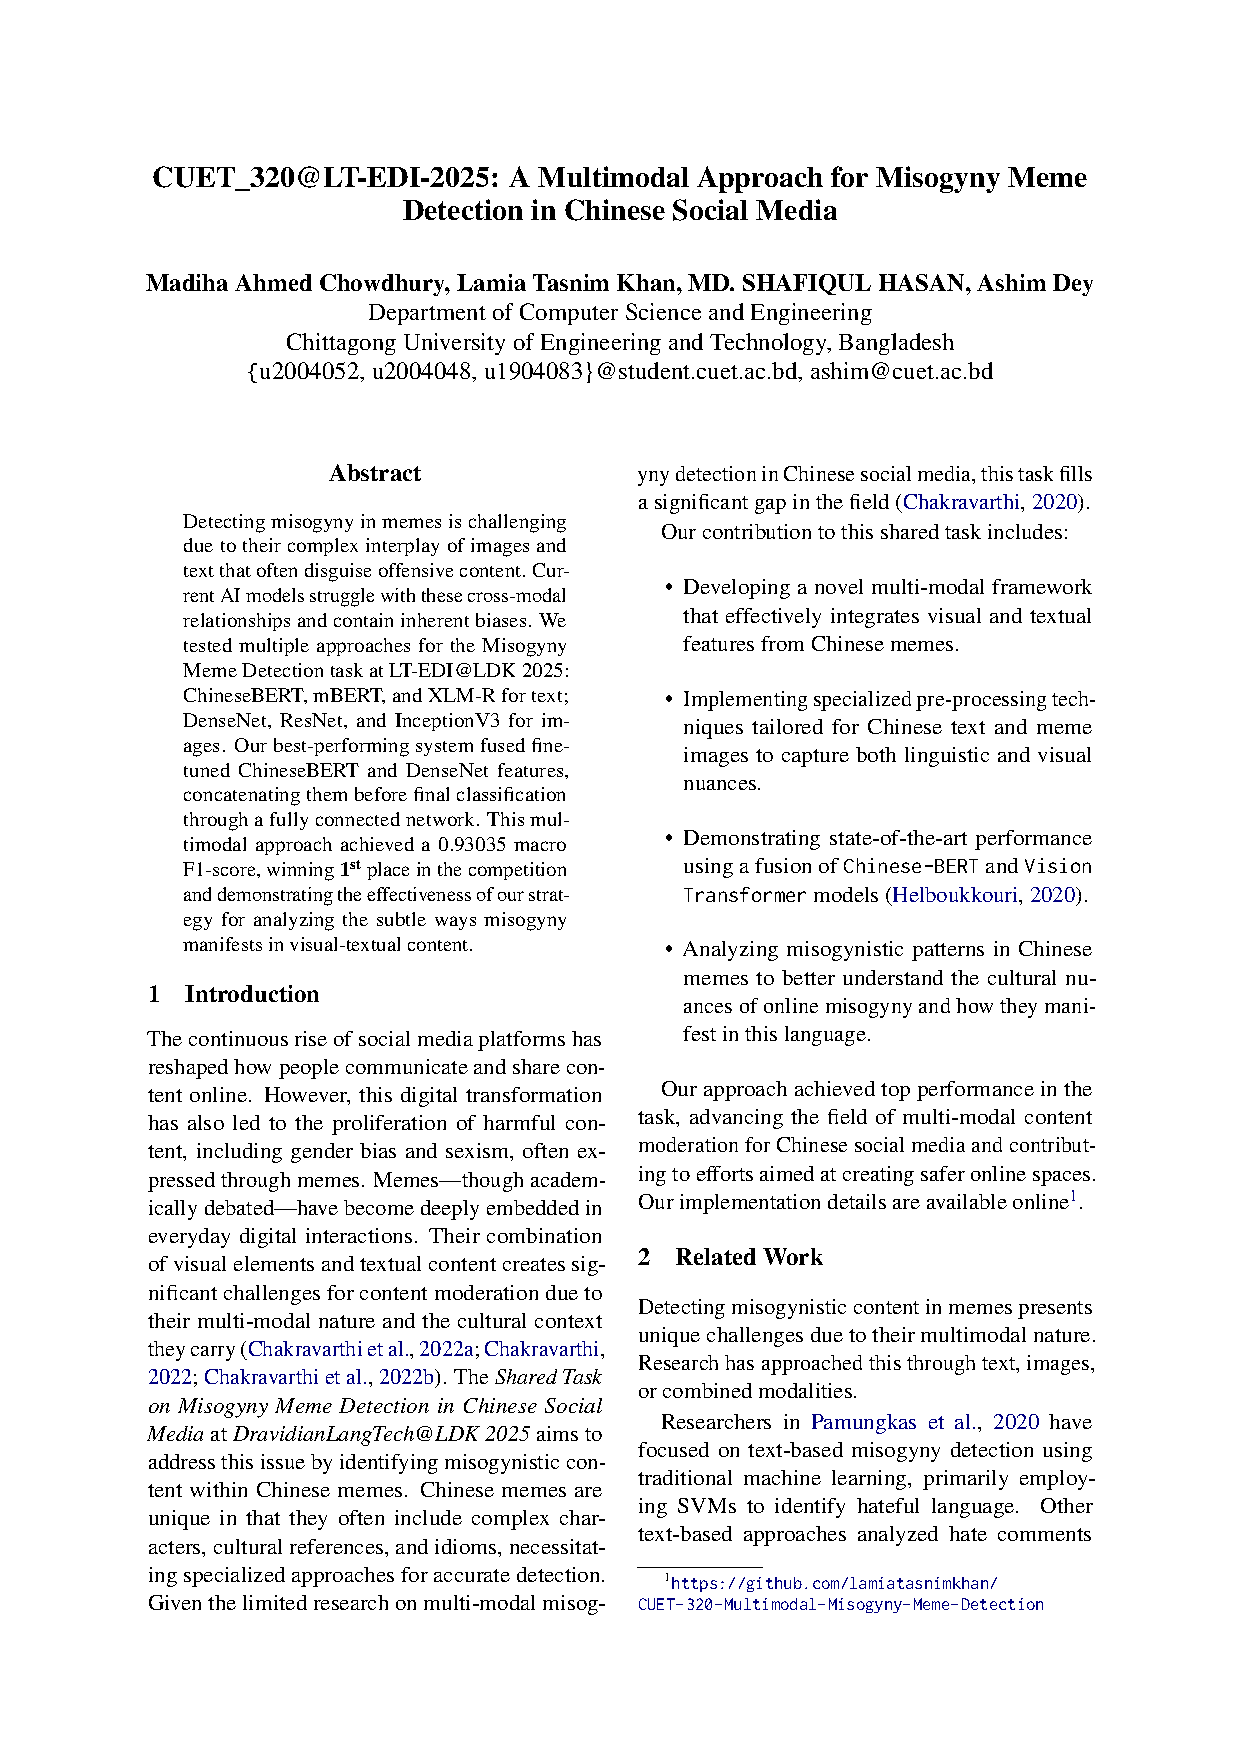
\includepdf[pagecommand={\thispagestyle{plain}},pages=-,addtotoc={1,section,1,{CUET\_320@LT-EDI-2025: A Multimodal Approach for Misogyny Meme Detection in Chinese Social Media},ref:paper_{33}}]{LT-EDI-2025/papers/33.pdf}
  \AddToShipoutPicture*{
    \setlength{\unitlength}{1mm}
    \footnotesize

            
    \put(0,13){\parbox[t]{\paperwidth}{\centering
    							\emph{Proceedings of the Fifth Workshop on Language Technology for Equality, Diversity, Inclusion}, pages 189--198 \\
  	  						September 9, 2025 \textcopyright
  							2025 Association for Computational Linguistics}}
  }
  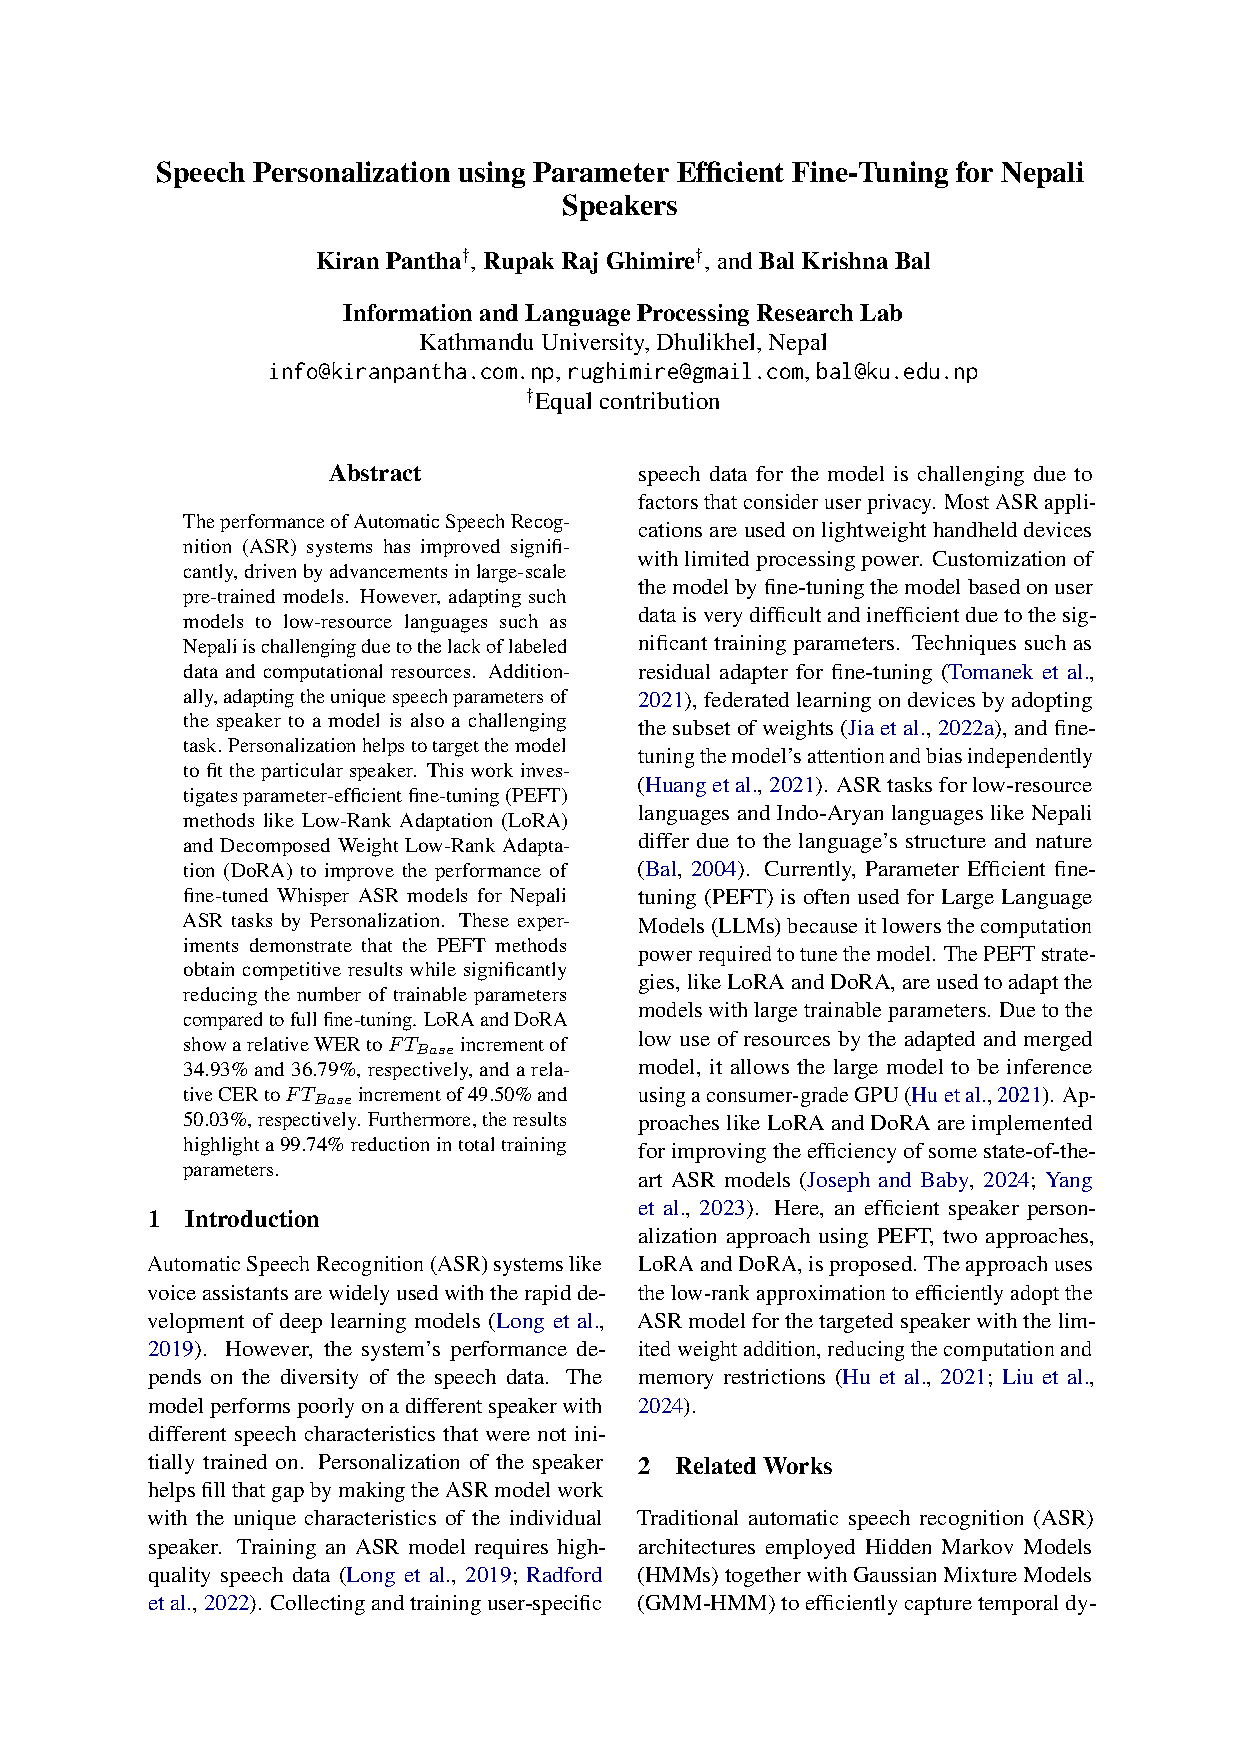
\includepdf[pagecommand={\thispagestyle{plain}},pages=-,addtotoc={1,section,1,{Speech Personalization using Parameter Efficient Fine-Tuning for Nepali Speakers},ref:paper_{34}}]{LT-EDI-2025/papers/34.pdf}
  \AddToShipoutPicture*{
    \setlength{\unitlength}{1mm}
    \footnotesize

            
    \put(0,13){\parbox[t]{\paperwidth}{\centering
    							\emph{Proceedings of the Fifth Workshop on Language Technology for Equality, Diversity, Inclusion}, pages 199--207 \\
  	  						September 9, 2025 \textcopyright
  							2025 Association for Computational Linguistics}}
  }
  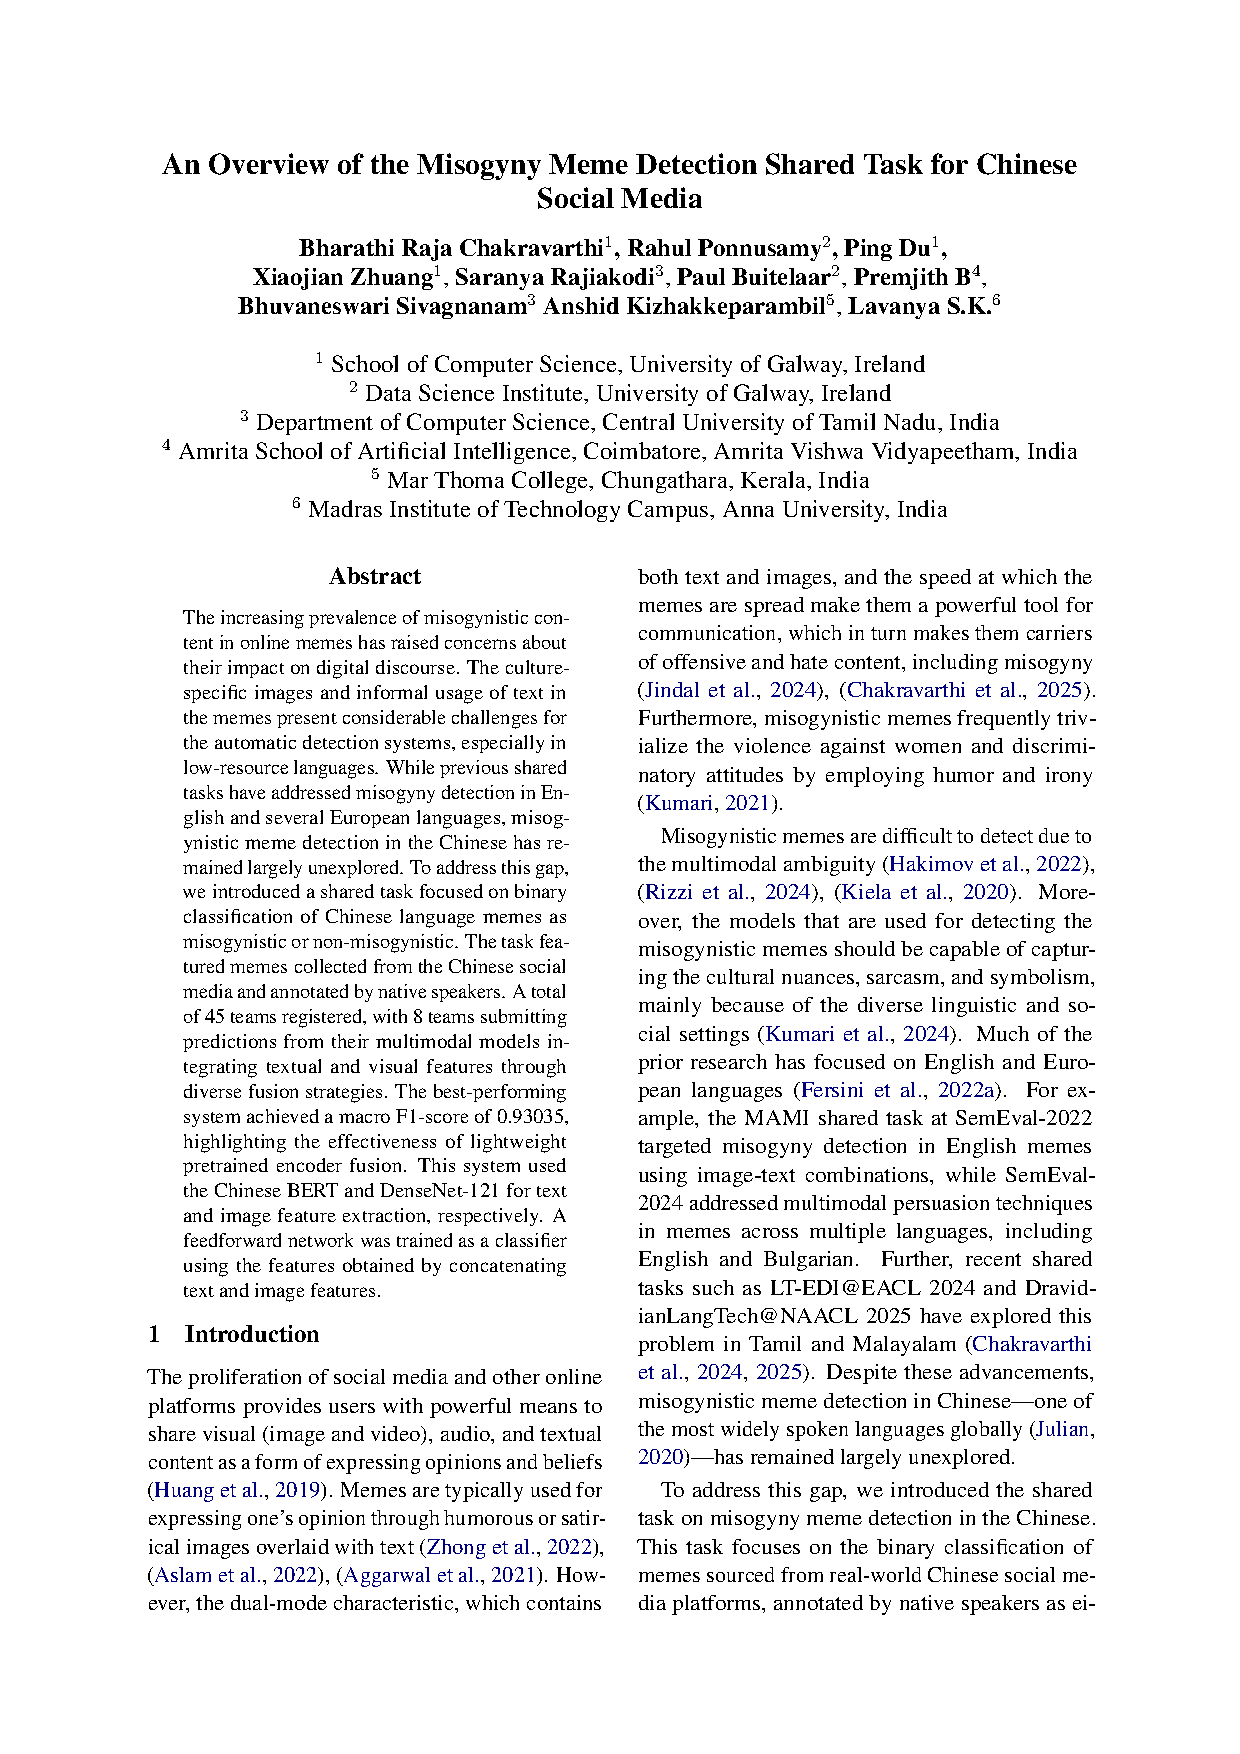
\includepdf[pagecommand={\thispagestyle{plain}},pages=-,addtotoc={1,section,1,{An Overview of the Misogyny Meme Detection Shared Task for Chinese Social Media},ref:paper_{35}}]{LT-EDI-2025/papers/35.pdf}
  \AddToShipoutPicture*{
    \setlength{\unitlength}{1mm}
    \footnotesize

            
    \put(0,13){\parbox[t]{\paperwidth}{\centering
    							\emph{Proceedings of the Fifth Workshop on Language Technology for Equality, Diversity, Inclusion}, pages 208--213 \\
  	  						September 9, 2025 \textcopyright
  							2025 Association for Computational Linguistics}}
  }
  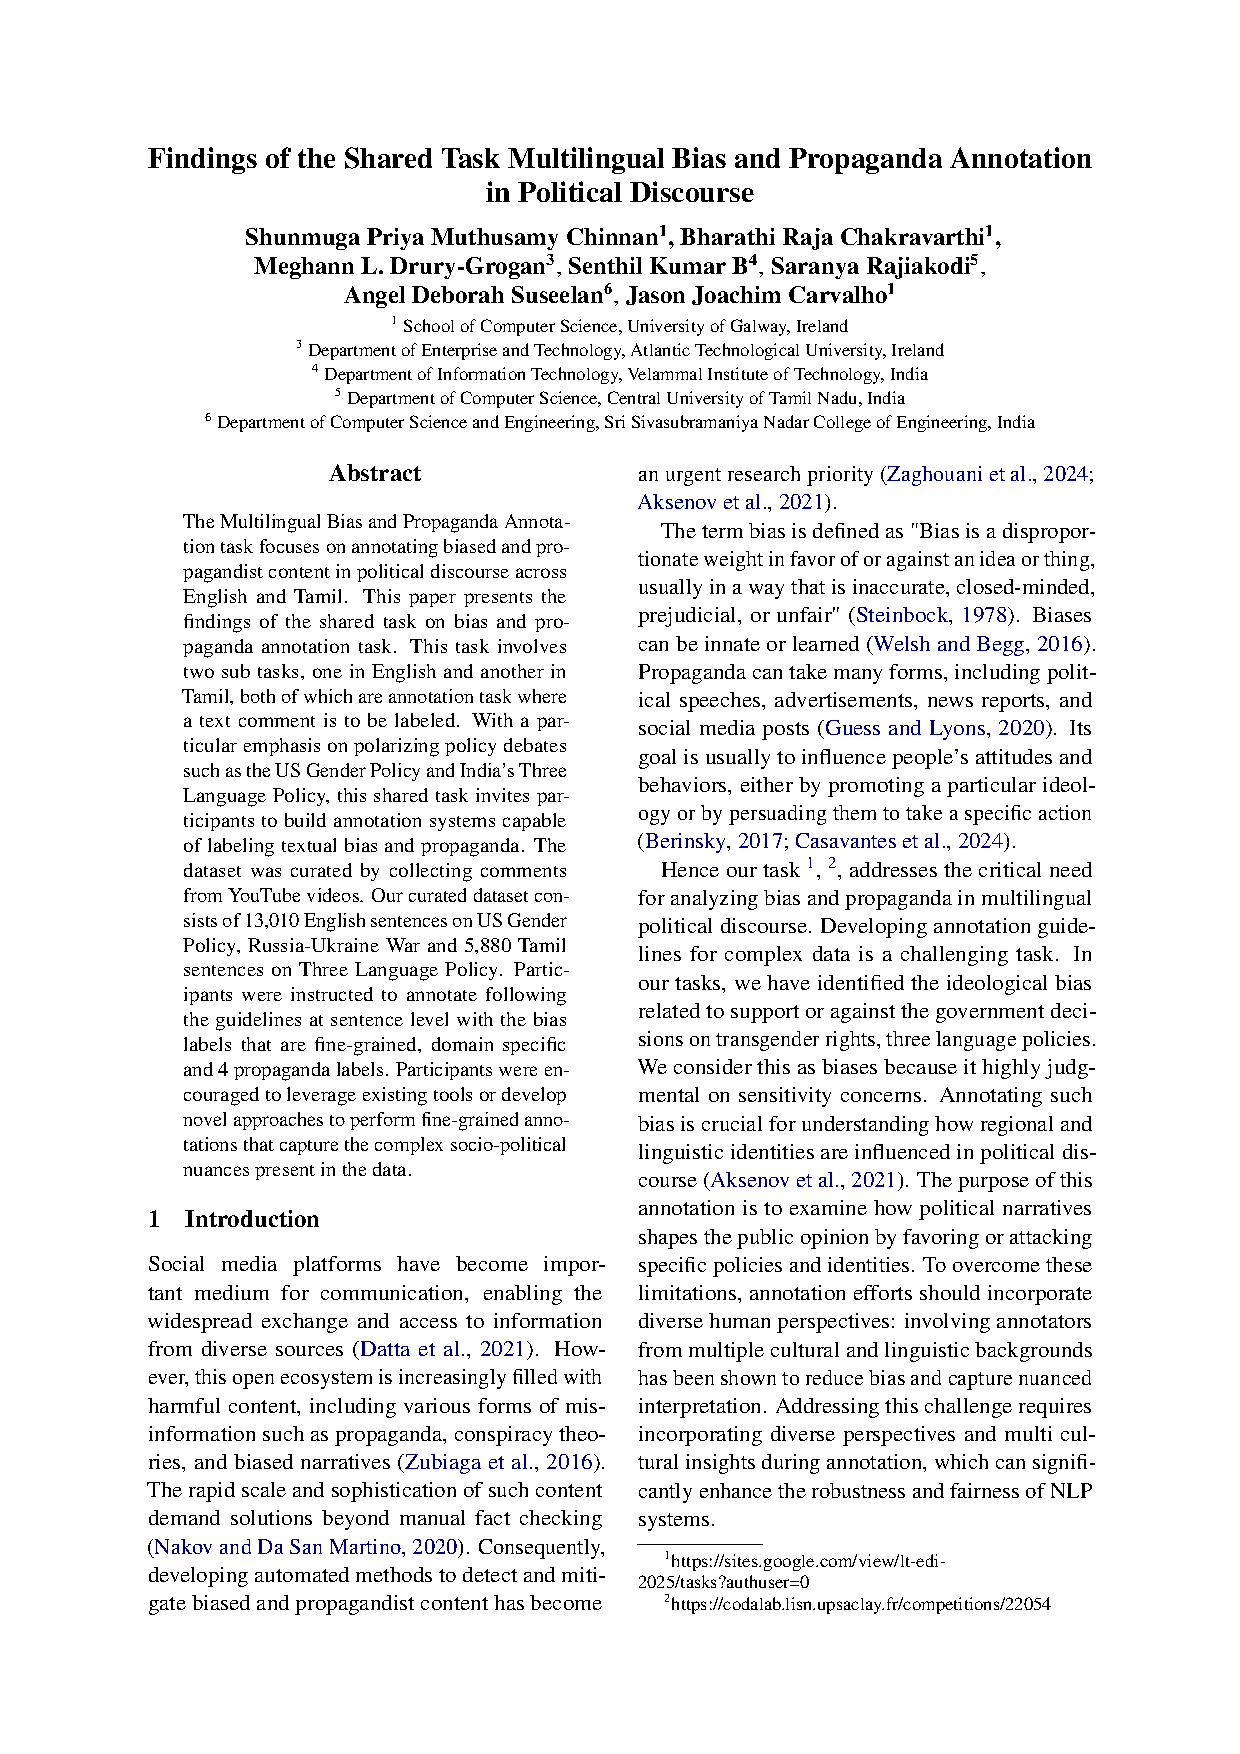
\includepdf[pagecommand={\thispagestyle{plain}},pages=-,addtotoc={1,section,1,{Findings of the Shared Task Multilingual Bias and Propaganda Annotation in Political Discourse},ref:paper_{36}}]{LT-EDI-2025/papers/36.pdf}
  \AddToShipoutPicture*{
    \setlength{\unitlength}{1mm}
    \footnotesize

            
    \put(0,13){\parbox[t]{\paperwidth}{\centering
    							\emph{Proceedings of the Fifth Workshop on Language Technology for Equality, Diversity, Inclusion}, pages 214--220 \\
  	  						September 9, 2025 \textcopyright
  							2025 Association for Computational Linguistics}}
  }
  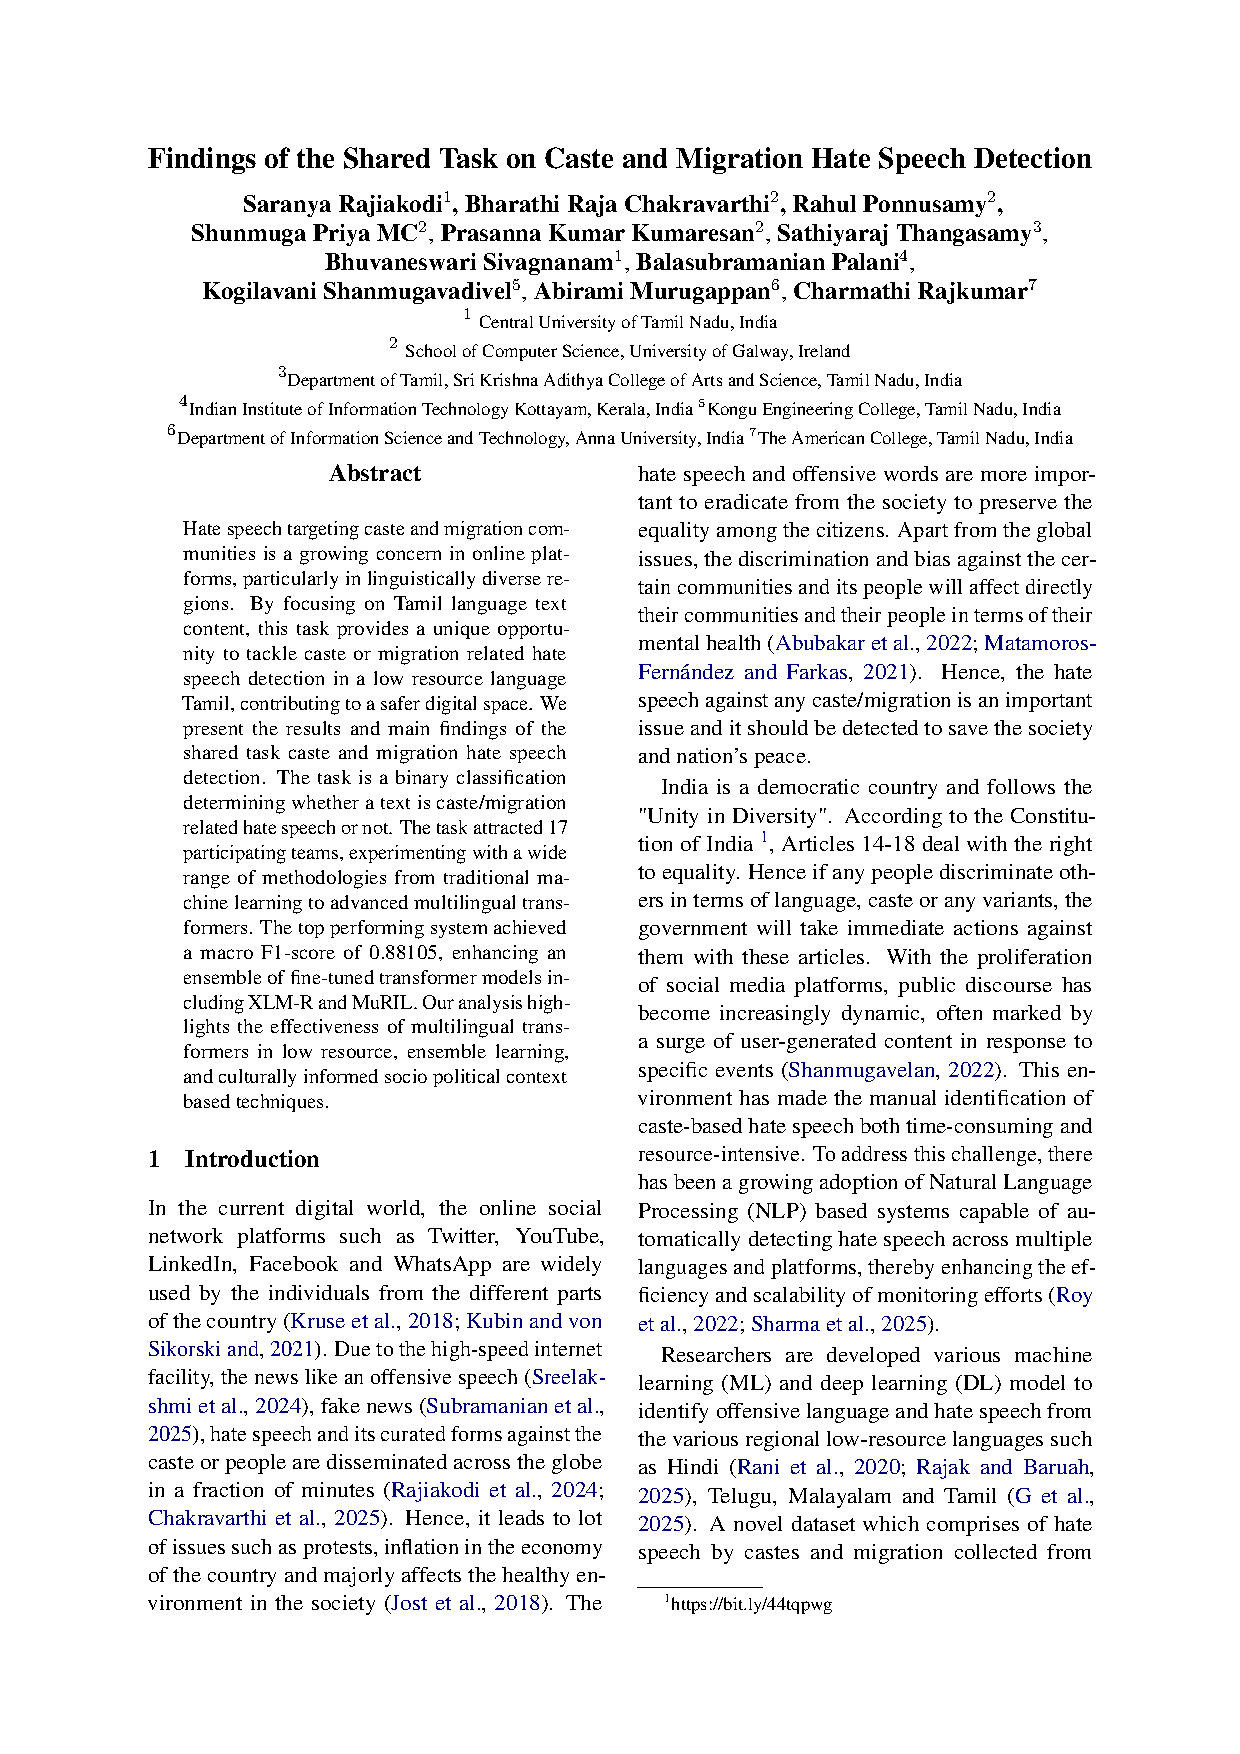
\includepdf[pagecommand={\thispagestyle{plain}},pages=-,addtotoc={1,section,1,{Findings of the Shared Task Caste and Migration Hate Speech Detection},ref:paper_{37}}]{LT-EDI-2025/papers/37.pdf}
  \AddToShipoutPicture*{
    \setlength{\unitlength}{1mm}
    \footnotesize

            
    \put(0,13){\parbox[t]{\paperwidth}{\centering
    							\emph{Proceedings of the Fifth Workshop on Language Technology for Equality, Diversity, Inclusion}, pages 221--227 \\
  	  						September 9, 2025 \textcopyright
  							2025 Association for Computational Linguistics}}
  }
  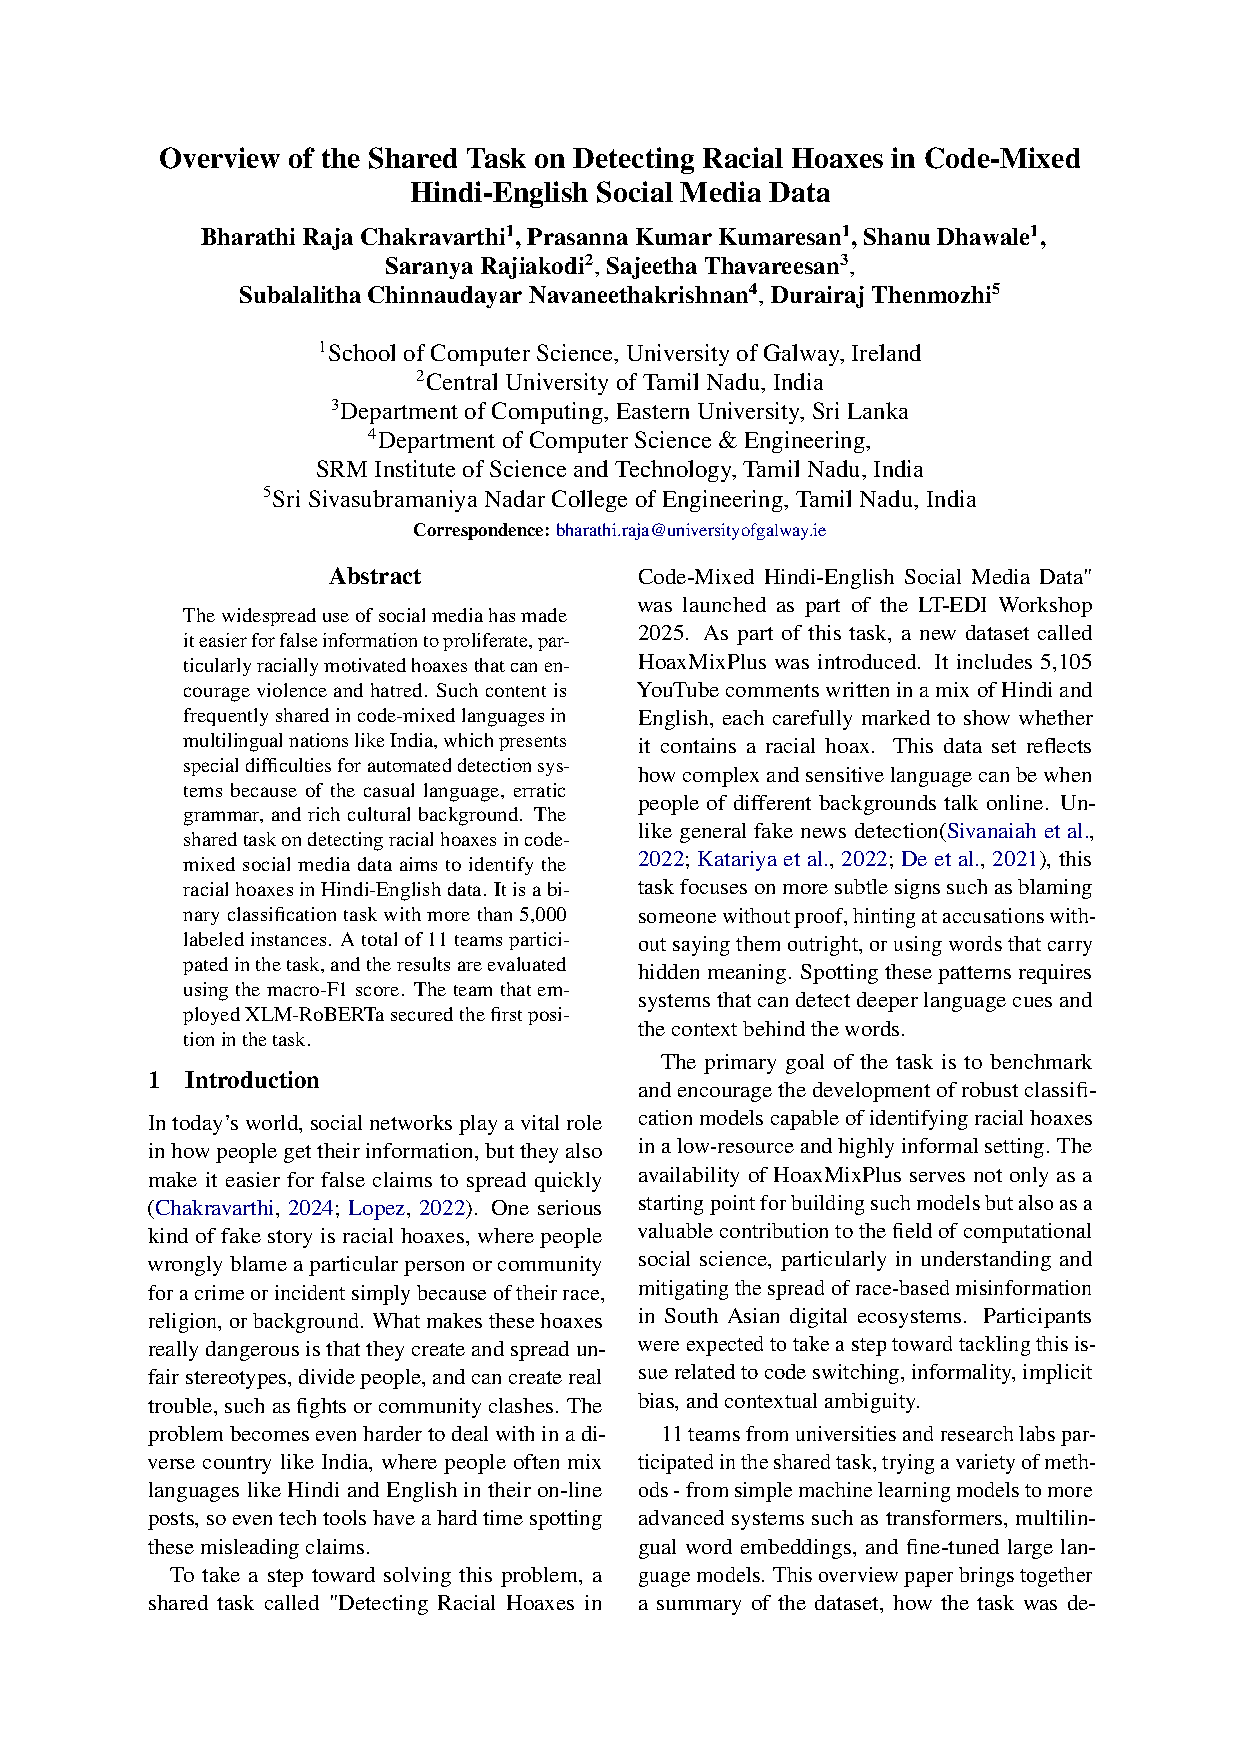
\includepdf[pagecommand={\thispagestyle{plain}},pages=-,addtotoc={1,section,1,{Overview of the Shared Task on Detecting Racial Hoaxes in Code-Mixed Hindi-English Social Media Data},ref:paper_{38}}]{LT-EDI-2025/papers/38.pdf}
  \AddToShipoutPicture*{
    \setlength{\unitlength}{1mm}
    \footnotesize

            
    \put(0,13){\parbox[t]{\paperwidth}{\centering
    							\emph{Proceedings of the Fifth Workshop on Language Technology for Equality, Diversity, Inclusion}, pages 228--233 \\
  	  						September 9, 2025 \textcopyright
  							2025 Association for Computational Linguistics}}
  }
  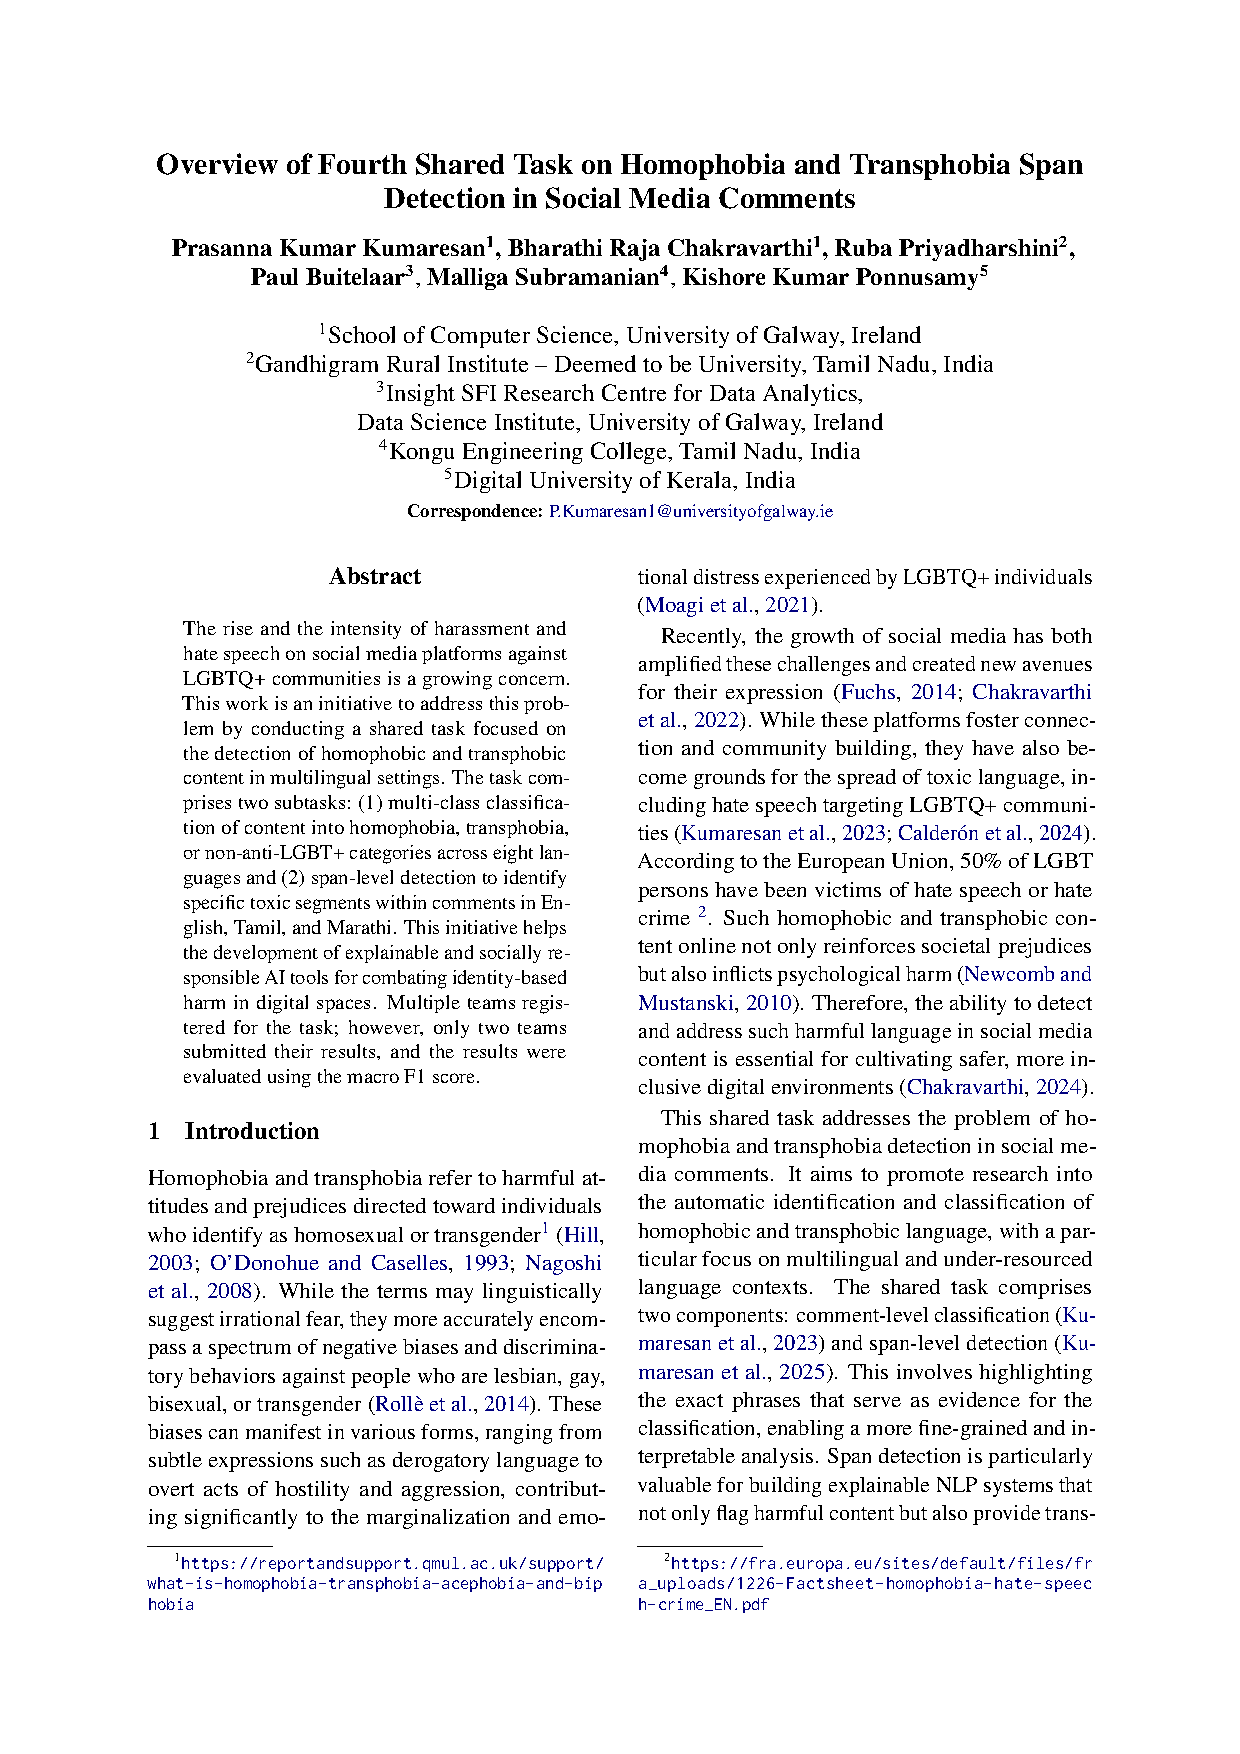
\includepdf[pagecommand={\thispagestyle{plain}},pages=-,addtotoc={1,section,1,{Overview of Homophobia and Transphobia Span Detection in Social Media Comments},ref:paper_{40}}]{LT-EDI-2025/papers/40.pdf}
  \AddToShipoutPicture*{
    \setlength{\unitlength}{1mm}
    \footnotesize

            
    \put(0,13){\parbox[t]{\paperwidth}{\centering
    							\emph{Proceedings of the Fifth Workshop on Language Technology for Equality, Diversity, Inclusion}, pages 234--240 \\
  	  						September 9, 2025 \textcopyright
  							2025 Association for Computational Linguistics}}
  }
  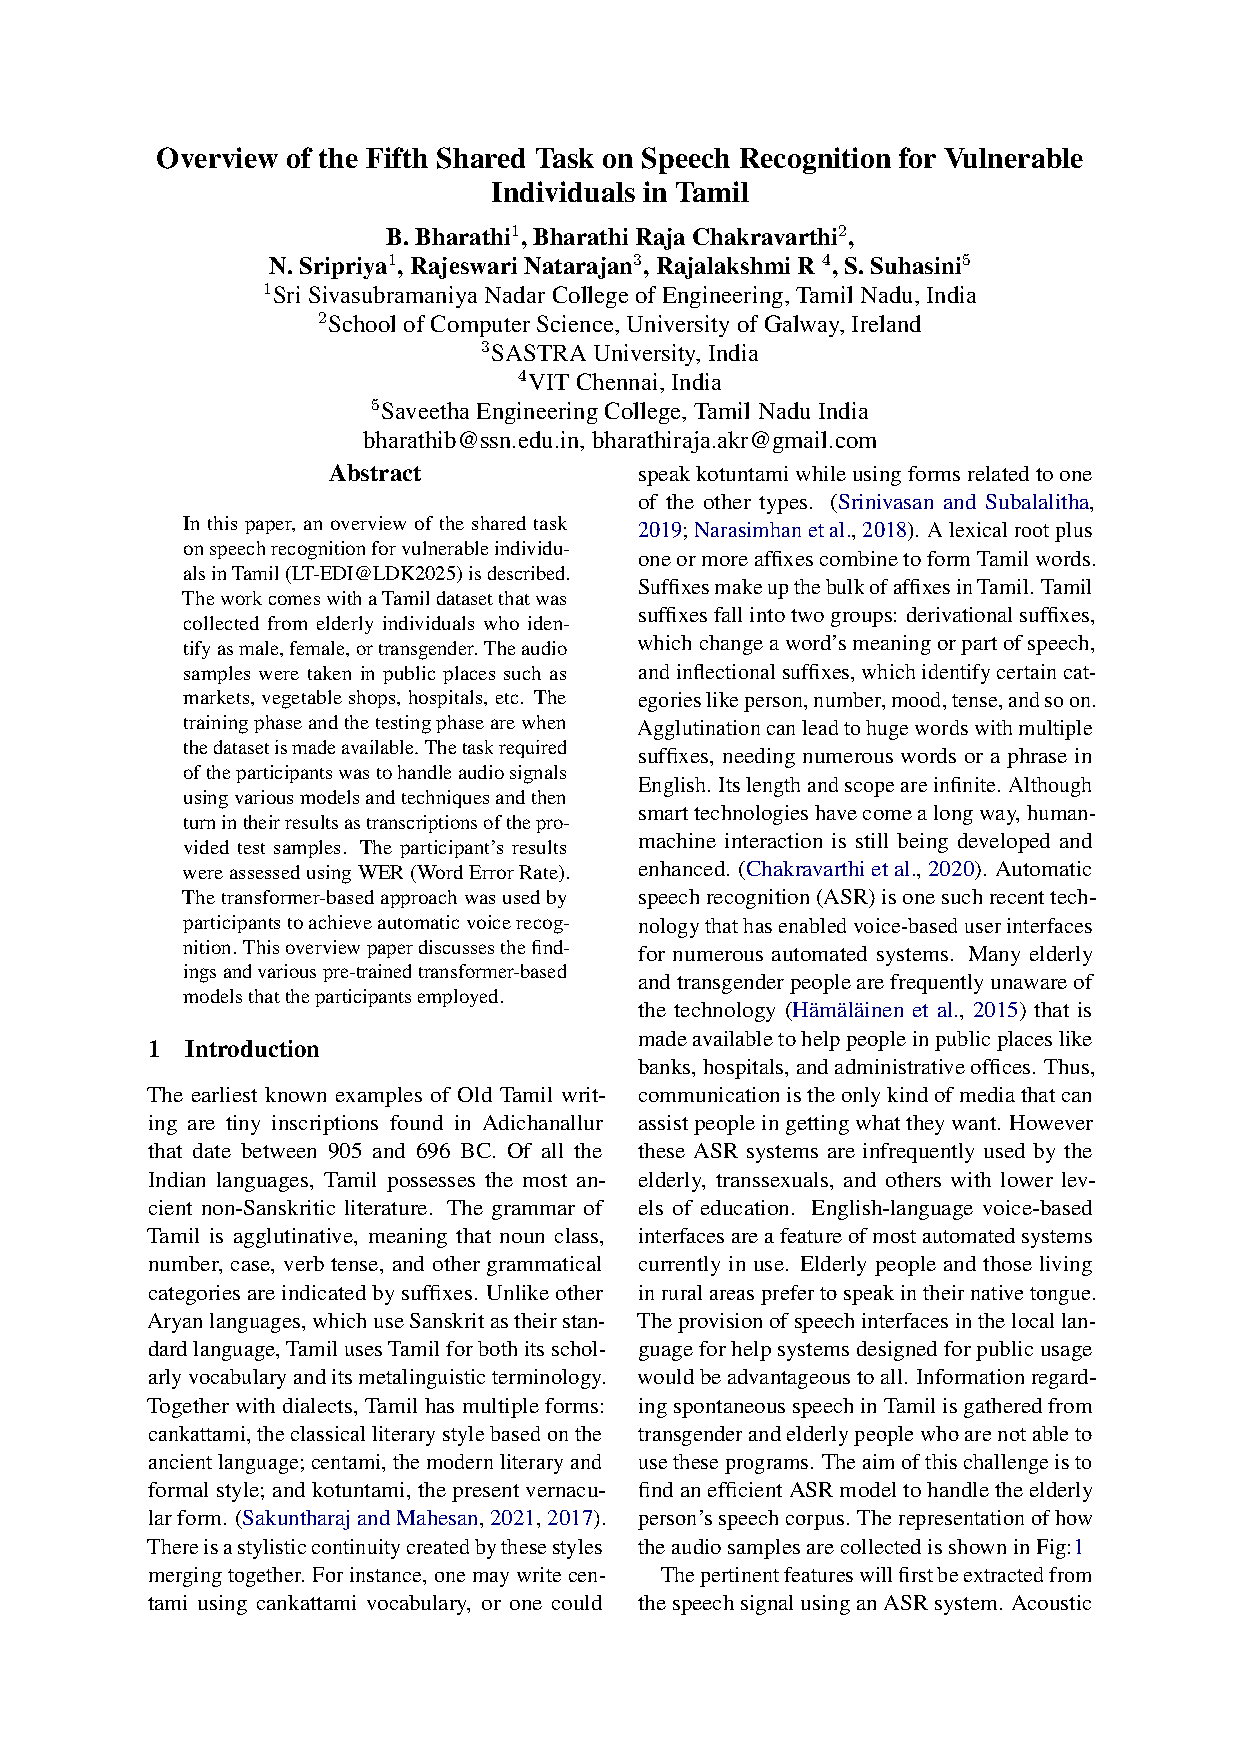
\includepdf[pagecommand={\thispagestyle{plain}},pages=-,addtotoc={1,section,1,{Overview of the Fifth Shared Task on Speech Recognition for Vulnerable Individuals in Tamil},ref:paper_{41}}]{LT-EDI-2025/papers/41.pdf}

%%%%%%%%%%%%%%%%
% Author Index %
%%%%%%%%%%%%%%%%
\begin{huge}
Author Index
\end{huge}
\vspace*{1em}
\begin{multicols}{2}
A, Anshid K, \hyperlink{page.199}{199}\\
A, Aruna, \hyperlink{page.111}{111}\\
A, Devasri, \hyperlink{page.100}{100}\\
Abiola, Tolulope Olalekan, \hyperlink{page.146}{146}, \hyperlink{page.152}{152}\\
Abrar, Jidan Al, \hyperlink{page.63}{63}, \hyperlink{page.68}{68}, \hyperlink{page.75}{75}\\
Achamaleh, Tewodros, \hyperlink{page.146}{146}, \hyperlink{page.152}{152}\\
Acharya, Priyobroto, \hyperlink{page.17}{17}\\
Aftahee, Sabik, \hyperlink{page.121}{121}, \hyperlink{page.140}{140}\\
Alam, Walisa, \hyperlink{page.177}{177}\\
Amin, MD AL, \hyperlink{page.121}{121}, \hyperlink{page.140}{140}\\
Arefin, Mohammad Shamsul, \hyperlink{page.68}{68}, \hyperlink{page.75}{75}, \hyperlink{page.171}{171}\\
\\ % Extra space between new letters.
B, Bharathi, \hyperlink{page.1}{1}, \hyperlink{page.6}{6}, \hyperlink{page.234}{234}\\
B, Premjith, \hyperlink{page.26}{26}, \hyperlink{page.199}{199}\\
B, Senthil Kumar, \hyperlink{page.208}{208}\\
Bal, Bal Krishna, \hyperlink{page.189}{189}\\
Buitelaar, Paul, \hyperlink{page.199}{199}, \hyperlink{page.228}{228}\\
\\ % Extra space between new letters.
C, Maria Nancy, \hyperlink{page.84}{84}\\
Chakravarthi, Bharathi Raja, \hyperlink{page.199}{199}, \hyperlink{page.208}{208}, \hyperlink{page.214}{214}, \hyperlink{page.221}{221}, \hyperlink{page.228}{228}, \hyperlink{page.234}{234}\\
Chaudhuri, Soham, \hyperlink{page.17}{17}\\
Chinnan, Shunmuga Priya Muthusamy, \hyperlink{page.208}{208}, \hyperlink{page.214}{214}\\
Chowdhury, Madiha Ahmed, \hyperlink{page.183}{183}\\
Chowdhury, Md. Tahfim Juwel, \hyperlink{page.105}{105}\\
Chowdhury, Shiti, \hyperlink{page.116}{116}\\
\\ % Extra space between new letters.
D, Arun Prasad T, \hyperlink{page.11}{11}\\
Das, Dipankar, \hyperlink{page.17}{17}\\
Das, Sayan, \hyperlink{page.17}{17}\\
Dey, Ashim, \hyperlink{page.183}{183}\\
Dhanush, MC, \hyperlink{page.54}{54}\\
Dhawale, Shanu, \hyperlink{page.221}{221}\\
Droba, Diganta Das, \hyperlink{page.159}{159}\\
Drury-Grogan, Meghann, \hyperlink{page.208}{208}\\
Du, Ping, \hyperlink{page.199}{199}\\
Durairaj, Thenmozhi, \hyperlink{page.221}{221}\\
\\ % Extra space between new letters.
Faisal, Adnan, \hyperlink{page.116}{116}\\
Fariha, Faozia, \hyperlink{page.127}{127}\\
\\ % Extra space between new letters.
G, Gnanasabesan, \hyperlink{page.54}{54}\\
G, Jyothish Lal, \hyperlink{page.11}{11}, \hyperlink{page.95}{95}\\
Getachew, Sara, \hyperlink{page.146}{146}, \hyperlink{page.152}{152}\\
Ghimire, Rupak Raj, \hyperlink{page.189}{189}\\
\\ % Extra space between new letters.
Hafeez, Nida, \hyperlink{page.146}{146}\\
Hasan, Md Mehedi, \hyperlink{page.68}{68}, \hyperlink{page.75}{75}\\
Hasan, Md.shafiqul, \hyperlink{page.183}{183}\\
\\ % Extra space between new letters.
Ilman, Rehenuma, \hyperlink{page.177}{177}\\
Islam, Ariful, \hyperlink{page.63}{63}, \hyperlink{page.75}{75}\\
\\ % Extra space between new letters.
K, Durai Singh, \hyperlink{page.54}{54}\\
K, Sitara, \hyperlink{page.47}{47}\\
K, Sreeja, \hyperlink{page.1}{1}, \hyperlink{page.6}{6}\\
Karim, Shahriar Farhan, \hyperlink{page.133}{133}\\
Kashmary, Anower Sha Shajalal, \hyperlink{page.133}{133}\\
Kawser, Md Siddikul Imam, \hyperlink{page.63}{63}, \hyperlink{page.68}{68}\\
Keerthana, Dondluru, \hyperlink{page.26}{26}\\
Khan, Lamia Tasnim, \hyperlink{page.183}{183}\\
Khan, Md Sajid Hossain, \hyperlink{page.140}{140}\\
Krishna, Mahankali Sri Ram, \hyperlink{page.26}{26}\\
Kumaresan, Prasanna Kumar, \hyperlink{page.214}{214}, \hyperlink{page.221}{221}, \hyperlink{page.228}{228}\\
\\ % Extra space between new letters.
L, Amritha Nandini K, \hyperlink{page.90}{90}\\
Labib, Momtazul Arefin, \hyperlink{page.116}{116}, \hyperlink{page.159}{159}\\
Lavanya, SK, \hyperlink{page.199}{199}\\
\\ % Extra space between new letters.
M, Amudhavan, \hyperlink{page.111}{111}\\
Mebraihtu, Mikiyas, \hyperlink{page.146}{146}, \hyperlink{page.152}{152}\\
Murad, Hasan, \hyperlink{page.63}{63}, \hyperlink{page.105}{105}, \hyperlink{page.116}{116}, \hyperlink{page.127}{127}, \hyperlink{page.133}{133}, \hyperlink{page.159}{159}\\
Murugappan, Abirami, \hyperlink{page.214}{214}\\
\\ % Extra space between new letters.
N, Hari Krishnan, \hyperlink{page.11}{11}, \hyperlink{page.54}{54}\\
N, Radha, \hyperlink{page.84}{84}\\
N, Sripriya, \hyperlink{page.234}{234}\\
Naib, Md. Mubasshir, \hyperlink{page.63}{63}, \hyperlink{page.68}{68}, \hyperlink{page.75}{75}\\
Natarajan, Rajeswari, \hyperlink{page.234}{234}\\
Navaneethakrishnan, Subalalitha Chinnaudayar, \hyperlink{page.221}{221}\\
Nishanth.S, Nishanth.S, \hyperlink{page.80}{80}, \hyperlink{page.95}{95}\\
\\ % Extra space between new letters.
Oman, Mohammad, \hyperlink{page.171}{171}\\
\\ % Extra space between new letters.
P, Bharath, \hyperlink{page.100}{100}\\
Palani, Balasubramanian, \hyperlink{page.214}{214}\\
Pantha, Kiran, \hyperlink{page.189}{189}\\
Ponnusamy, Kishore Kumar, \hyperlink{page.228}{228}\\
Ponnusamy, Rahul, \hyperlink{page.199}{199}, \hyperlink{page.214}{214}\\
Priyadharshini, Ruba, \hyperlink{page.228}{228}\\
\\ % Extra space between new letters.
Quintero, Rolando, \hyperlink{page.146}{146}\\
\\ % Extra space between new letters.
R, Giri Prasath, \hyperlink{page.90}{90}\\
R, Swathika, \hyperlink{page.84}{84}\\
Rabbani, Abrar Hafiz, \hyperlink{page.159}{159}\\
Rahman, Md Ashiqur, \hyperlink{page.121}{121}, \hyperlink{page.140}{140}\\
Rahman, Md Mizanur, \hyperlink{page.63}{63}, \hyperlink{page.68}{68}, \hyperlink{page.75}{75}\\
Rahman, Md. Abdur, \hyperlink{page.121}{121}, \hyperlink{page.140}{140}\\
Rahman, MD.Mahadi, \hyperlink{page.171}{171}\\
Rahman, Mehreen, \hyperlink{page.127}{127}\\
Rahman, Samia, \hyperlink{page.127}{127}, \hyperlink{page.159}{159}, \hyperlink{page.177}{177}\\
Rahul, Burugu, \hyperlink{page.95}{95}\\
Rajalakshmi, Ratnavel, \hyperlink{page.234}{234}\\
Rajiakodi, Saranya, \hyperlink{page.199}{199}, \hyperlink{page.208}{208}, \hyperlink{page.214}{214}, \hyperlink{page.221}{221}\\
Rajkumar, Charmathi, \hyperlink{page.214}{214}\\
Rengarajan, Shruthi, \hyperlink{page.80}{80}, \hyperlink{page.95}{95}\\
Ruman, Md. Nur Siddik, \hyperlink{page.105}{105}\\
\\ % Extra space between new letters.
S, Ananthakumar, \hyperlink{page.100}{100}\\
S, Angel Deborah, \hyperlink{page.208}{208}\\
S, Anirudh Sriram K, \hyperlink{page.100}{100}\\
S, Ganesh Sundhar, \hyperlink{page.11}{11}, \hyperlink{page.54}{54}\\
S, Jahaganapathi, \hyperlink{page.111}{111}\\
S, Sachin Kumar, \hyperlink{page.80}{80}, \hyperlink{page.90}{90}\\
S, Suhasini, \hyperlink{page.234}{234}\\
S, Vishal, \hyperlink{page.90}{90}\\
Saha, Dipanjan, \hyperlink{page.17}{17}\\
Shanmugavadivel, Kogilavani, \hyperlink{page.111}{111}, \hyperlink{page.214}{214}\\
Sharma, Deepawali, \hyperlink{page.39}{39}\\
Sidorov, Grigori, \hyperlink{page.146}{146}, \hyperlink{page.152}{152}\\
Singh, Aakash, \hyperlink{page.39}{39}\\
Singh, Vivek Kumar, \hyperlink{page.39}{39}\\
Singh, Vrijendra, \hyperlink{page.31}{31}\\
Sivagnanam, Bhuvaneswari, \hyperlink{page.199}{199}, \hyperlink{page.214}{214}\\
Subramanian, Malliga, \hyperlink{page.111}{111}, \hyperlink{page.228}{228}\\
\\ % Extra space between new letters.
T, Mohanapriya K, \hyperlink{page.100}{100}\\
T, Radhika K, \hyperlink{page.47}{47}\\
Tabassum, Nabilah, \hyperlink{page.127}{127}\\
Thangasamy, Sathiyaraj, \hyperlink{page.214}{214}\\
Thavareesan, Sajeetha, \hyperlink{page.221}{221}\\
Thiyagarajan, Anerud, \hyperlink{page.90}{90}\\
Tushi, Towshin HOssain, \hyperlink{page.177}{177}\\
\\ % Extra space between new letters.
Uddin, Mohammad Minhaj, \hyperlink{page.171}{171}\\
Uroosa, Fatima, \hyperlink{page.146}{146}\\
\\ % Extra space between new letters.
V, Shruthikaa, \hyperlink{page.11}{11}\\
Vignesh, Konkimalla Laxmi, \hyperlink{page.26}{26}\\
\\ % Extra space between new letters.
Yadav, Abhishek Singh, \hyperlink{page.39}{39}\\
Yadav, Ashok, \hyperlink{page.31}{31}\\
\\ % Extra space between new letters.
Zhuang, Xiaojian, \hyperlink{page.199}{199}\\
\\ % Extra space between new letters.
\end{multicols}


\end{document}